%\documentclass{article}
\documentclass[12pt]{article}
\usepackage{times}
%\usepackage{natbib}
%\usepackage{multicol}
\RequirePackage{natbib}
\usepackage{amsmath, amssymb, fullpage, amsthm, array, algorithm2e,graphicx,asa}
%\usepackage[dvips]{graphics}
\usepackage{hyperref}

\graphicspath{{images/}}
\usepackage{color}
\newcommand{\blue}[1]{{\color{blue} #1}} %MM
\newcommand{\red}[1]{{\color{red} #1}} 
\newcommand{\green}[1]{{\color{green} #1}} %DC

\definecolor{orange}{rgb}{1,0.5,0}
\newcommand{\hh}[1]{{\color{orange} #1}} %HH

% \usepackage{pifont} % this package is used to print check mark \checkmark
%\linespread{2}


\setlength{\oddsidemargin}{0in}
\setlength{\evensidemargin}{0in}
\setlength{\textwidth}{6.5in}
\setlength{\topmargin}{-0.4in}
\setlength{\textheight}{9in}
\evensidemargin 
\oddsidemargin

\newtheorem{thm}{Theorem}[section]
\newtheorem{dfn}{Definition}[section]
\newtheorem{cor}{Corollary}[thm]
\newtheorem{con}{Conjecture}[thm]
\newtheorem{lemma}[thm]{Lemma}

%\topmargin -0.10in   % when making pdf
%\textheight 9.15in  % when making pdf

\begin{document}

% Article top matter
\title{Validation of Visual Statistical Inference, Applied to Linear Models}
\author{
{Mahbubul Majumder, Heike Hofmann, Dianne Cook}
\thanks{Mahbubul Majumder is Graduate Student (e-mail: mahbub72@gmail.com) , Heike Hofmann is Associate  Professor and Dianne Cook is Full Professor, Department of
Statistics and Statistical Laboratory, Iowa State University,
Ames, IA 50011-1210. This research is supported in part by the
National Science Foundation Grant \# DMS 1007697.}}
\date{\vspace{-.7in}}
%\date{\today}  %\today is replaced with the current date
\maketitle

\begin {abstract}  
Statistical graphics play a crucial role in exploratory data analysis, model checking and diagnosis. Until recently, there were no formal visual methods in place for determining statistical significance of findings. This changed when \citet{buja:2009} conceptually introduced the lineup protocol for formal tests of visual findings. In this paper this is taken a step further by refining the terminology of visual inference, framing the protocol in a context that allows direct comparison with conventional tests, in scenarios when a conventional test exists, and it is used to compare the performance of the lineup protocol against conventional statistical testing in the scenario of fitting linear models. A human subjects experiment is conducted using simulated data to provide controlled conditions. Results suggest that the lineup protocol provides results comparable to the conventional tests, out-performs them when data is contaminated, and, there may be some super-individuals who yield better power than the conventional test even in the most difficult trials.

{\bf Keywords: \sf statistical graphics, lineup, non-parametric test, data mining, visualization, exploratory data analysis} 
\end {abstract}

%\begin{multicols}{2}
%\twocolumn

\section{Introduction} 

%\checkmark

Statistical graphics nourish the discovery process in data analysis by revealing unexpected things,  finding structure that was not previously anticipated,  or orthogonally by contrasting prevailing hypotheses. The area of graphics is often associated with exploratory data analysis, which was pioneered by \cite{tukey:eda} and, is particularly pertinent in today's data-rich world where discovery during data mining has become an important activity. Graphics are also used in many places where numerical summaries simply do not suffice: model checking, diagnosis, and in the communication of findings. 

Statistical graphics research and development is agreeably established now, and has been cemented by several new developments in recent years. Early studies on evaluating how well statistical plots are perceived and read by the human eye \citep{cleveland:1984}, have been repeated and expanded \citep{simkin:1987,spence:1991, heer:2010} with findings supporting the original results. This body of work provides a framework for evaluating new statistical graphics.  In a complementary direction, new research on formalizing statistical graphics with language characteristics makes it easier to abstractly define, compare and contrast data plots. \cite{wilkinson:1999} developed a grammar of graphics that is enhanced by \cite{hadley:2009}. These methods provide a mechanism to abstract the way data is mapped to graphical form. Finally, technology advances make it simple and easy for everyone to draw plots of data, and particularly the existence of software systems, such as R \citep{R}, enable making beautiful data graphics that can be tightly coupled with statistical modeling.

However, measuring the strength of patterns seen in plots, and differences in individual perceptual ability, is something that is difficult and perhaps handicaps graphics  use among statisticians, where measuring probabilities is of primary importance. This has also been addressed in recent research. \citet{buja:2009} proposes a protocol that allows the testing of discoveries made from statistical graphics. This work represents a major advance for graphics, because it bridges the gulf between conventional statistical inference procedures and exploratory data analysis. One of the protocols, the lineup, places the actual data plot among  a page of plots of null data, and asks a human judge to pick the plot that is different. Figure \ref{fig:test_category} shows an example lineup. Which plot do you think is the most different from the others? (The position of the actual data plot is provided in Section \ref{sec:category}.) Wrapped in a process that mirrors conventional inference, where there is an explicit, a priori, null hypothesis, picking the plot of the data from the null plots represents a rejection of that null hypothesis. The null hypothesis typically derives from the task at hand, or the type of plot being made. The alternative encompasses all possible antitheses, all types of patterns that might be detected in the actual data plot, accounting for all possible deviations from the null without the requirement to specify these ahead of time. The probability of rejection can be quantified, along with Type I, and Type II error, and $p$-value and power can be defined and estimated. 


\begin{figure}[htp]
%\begin{figurehere}
   \centering
       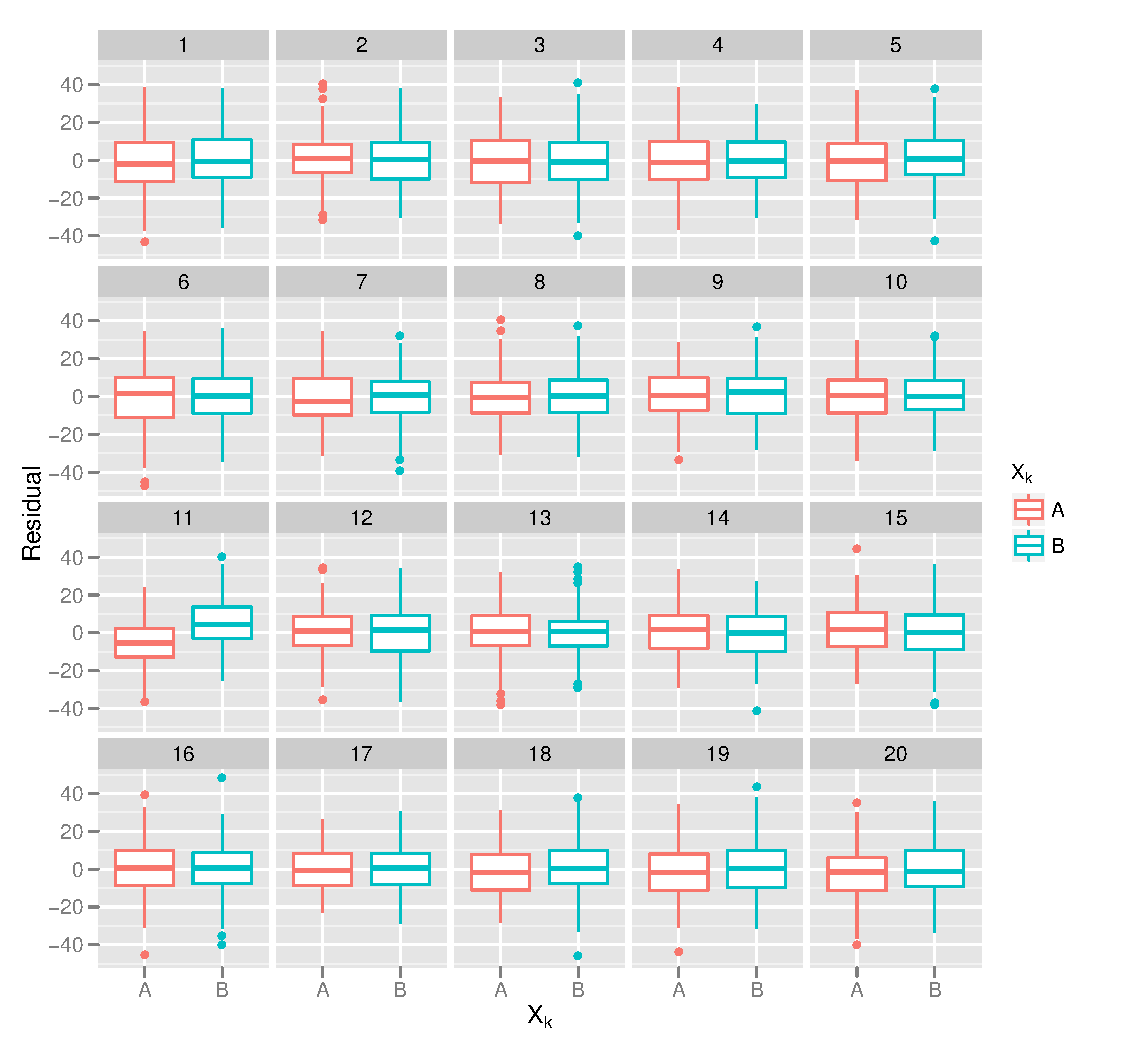
\includegraphics[width=0.95\textwidth]{lineup_category.pdf}
       \caption{Lineup plot ($m=20$) using side-by-side boxplots for testing $H_0: \beta_k=0$. One of these plots is the plot of the actual data, and the remaining are null plots, produced by simulating data from a null model that assumes $H_0$ is true. Which plot is the most different from the others, in the sense that there is the largest shift or location difference between the boxplots? (The position of the actual data plot is provided in Section \ref{sec:category}.)}
       \label{fig:test_category}
\end{figure}
%\end{figurehere}

The protocol has only been informally tested until now. In the work described in this paper, the lineup protocol is compared head to head with the equivalent conventional test. Specifically, the lineup is examined in the context of a linear model setting, where we are determining the importance of including a variable in the model. This is not the envisioned environment for the use of the lineup -- actually it is likely the worst case scenario for visual inference. The intended use of lineups is where there is no existing test, and unlikely to be ever any numerical test. The thought is though, that the conventional setting provides a benchmark for how well the lineup protocol works under controlled conditions, and will provide some assurance that they will work in scenarios where there is no benchmark. Testing is done based on a human-subjects experiment using Amazon's Mechanical Turk \citep{turk}, using simulation to provide controlled conditions for assessing lineups. The results are compared with those of the conventional test. 

%, analysis requires plots of data. For exploratory data analysis, statistical graphics play an invaluable role in model checking and diagnostics. Even though we have established mathematical procedures to obtain various statistics, we need to support the results by also producing the relevant plots. 

%The scientific foundation of graphical methods for data analysis is well established by \cite{cleveland:1984}. In recent years we have seen several major advances in statistical graphics. Modern computing systems like R and SAS ease the production of high quality statistical plots. A grammar of graphics introduced by \cite{wilkinson:1999} presents a structured way to generate specific graphics from data and define connections between disparate types of plots.  \cite{hadley:2009} has implemented a revised version of the grammar of graphics in R, in the package {\tt ggplot2}.   \blue {Graham Wills has implemented the grammar in SPSS, but I'm not sure how to cite this.}


%\citet{buja:2009}, following from \cite{gelman:2004}, proposed two protocols that allow the testing of discoveries made from statistical graphics. This work represents a major advance for graphics, because it bridges the gulf between conventional statistical inference procedures and exploratory data analysis.

%In this paper we compare the lineup protocol to conventional statistical inference, specifically applied to the regression framework. We also present results of a human-subject study assessing the performance of individuals on lineup plots \citep{buja:2009} for testing significance of regression parameters. 

The paper is organized as follows. Section \ref{sec:visual_test} defines terms as used in visual inference, and describes how to estimate the important quantities from experimental data. The effect of the lineup size and number of observers on the power of the test is discussed in Section \ref{sec:size}. Section \ref{sec:regression} focuses on the application of  visual inference to linear models.  Section \ref{sec:simulation} describes the results of the three simulation experiments conducted to compare the power of the lineup protocol with the equivalent conventional test and an analysis of the resulting data. The last section describes the next steps in this research.


\section{Definitions and Explanations for Visual Statistical Inference} \label{sec:visual_test} 

Table \ref{tbl:compare} illustrates the lineup protocol in relation to conventional hypothesis testing. Both start from the same place, the same set of hypotheses. The conventional test statistic is the $t$-statistic, where the parameter estimate is divided by its standard error. In the lineup protocol, the test statistic is a plot of the data. Here, side-by-side boxplots are used, because the variable of interest is categorical and takes just two values. In conventional hypothesis testing the value of the test statistic is compared with all possible values of the sampling distribution, the distribution of the statistic if the null hypothesis is true. If it is extreme on this scale then the null hypothesis is rejected. In contrast in visual inference, the plot of the data is compared with plots of a finite number of samples drawn from the null distribution. If the actual data plot is selected as the most different, then this results in rejection of the null hypothesis.

\begin{table*}[hbtp]
\caption{Comparison of visual inference with conventional inference.}
\centering 
\begin{tabular}{llll} 
\hline \hline
  & Conventional Inference &  Lineup Protocol \\ %[0.5ex] % inserts table %heading 
\hline
  Hypothesis & $H_0: \beta=0$ vs $H_1: \beta > 0$& $H_0: \beta=0$ vs $H_1: \beta > 0$\\
 & \begin{minipage}[h]{2.5cm} \begin{center} \scalebox{0.2}{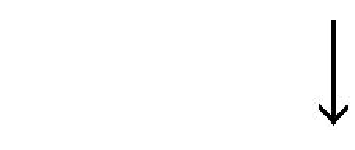
\includegraphics{down_arrow.pdf}} \end{center} \end{minipage} & \begin{minipage}[h]{2.5cm} \begin{center} \scalebox{0.2}{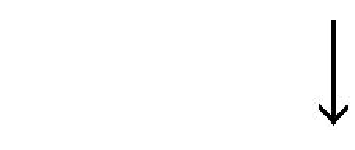
\includegraphics{down_arrow.pdf}} \end{center} \end{minipage} \\
				  
 Test statistic & $T(y)=\frac{\hat{\beta}}{se(\hat{\beta})}$ & $T(y)=$ \begin{minipage}[h]{1cm} \begin{center} \scalebox{0.45}{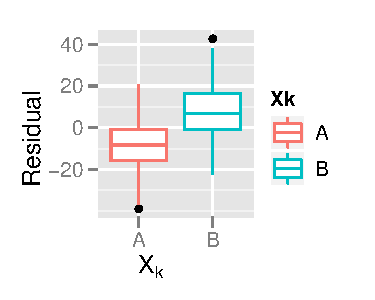
\includegraphics{stat_category.pdf}} \end{center} \end{minipage} \\
				 
 & \begin{minipage}[h]{2.5cm} \begin{center} \scalebox{0.2}{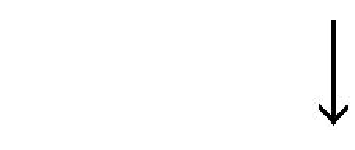
\includegraphics{down_arrow.pdf}} \end{center} \end{minipage} & \begin{minipage}[h]{2.5cm} \begin{center} \scalebox{0.2}{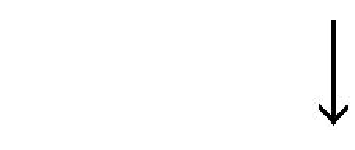
\includegraphics{down_arrow.pdf}} \end{center} \end{minipage} \\
				 
 Sampling Distribution & $f_{T(y)}(t); $\begin{minipage}[h]{2.5cm} \begin{center} \scalebox{0.55}{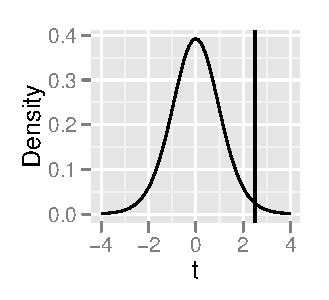
\includegraphics{stat_mathematical_test.pdf}} \end{center} \end{minipage} & $f_{T(y)}(t); $ \begin{minipage}[h]{2.5cm} \begin{center} \scalebox{0.32}{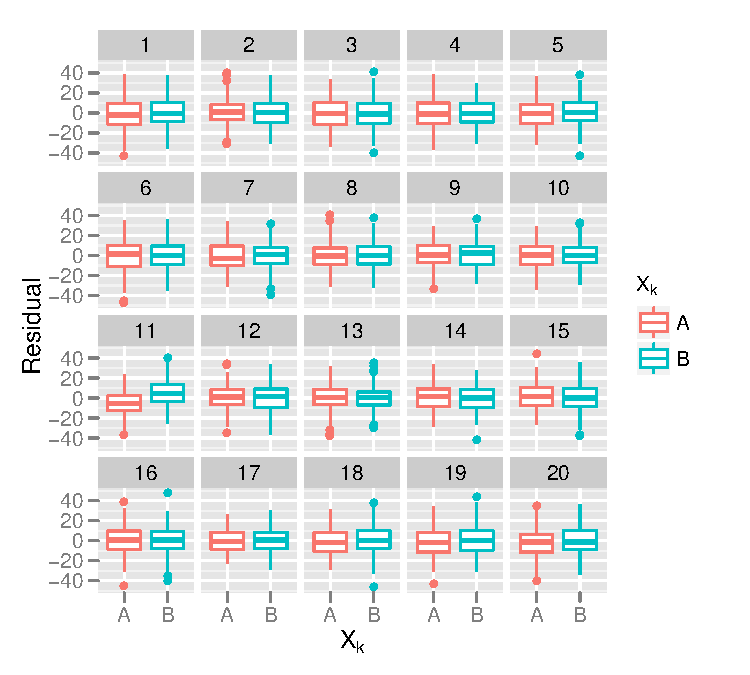
\includegraphics{lineup_category_small.pdf}} \end{center} \end{minipage} \\
 & \begin{minipage}[h]{2.5cm} \begin{center} \scalebox{0.2}{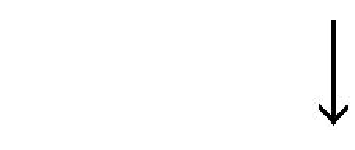
\includegraphics{down_arrow.pdf}} \end{center} \end{minipage} & \begin{minipage}[h]{2.5cm} \begin{center} \scalebox{0.2}{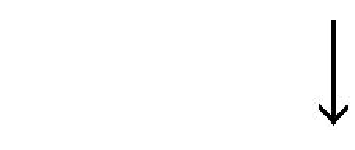
\includegraphics{down_arrow.pdf}} \end{center} \end{minipage} \\
 Reject $H_0$ if & actual $T$ is extreme & actual plot is identifiable \\
\hline 
\end{tabular}
\label{tbl:compare}
\end{table*}	


%Visual tests are non-parametric tests of the form $H_0$: the data plot is visually not distinguishable from a null plot vs $H_1$: the data plot is visually distinguishable from a plot generated consistently with $H_0$.

%Power of a plot and $p$-value have been derived in Buja and Wickham as ...



%for this paper, we want to place the parametric inference of a regression setting into the framework of visual testing:



%This section outlines the concepts of visual inference in comparison to the procedures of conventional statistical inference. Table \ref{tbl:compare} (derived from \citet{buja:2009}) gives a summarized overview of this comparison.

In general, we define $\theta$ to be a population parameter of interest, with $\theta \in \Theta$, the parameter space. Any null hypothesis $H_0$ then partitions the parameter space into $\Theta_0$ and $\Theta_0^c$, with $H_0: \theta \in \Theta_0$ versus $H_1: \theta \in \Theta_0^c$. A test statistic, $T(y)$, is a function that maps the sample into a numerical summary, that can be used to test the null hypothesis. The hypothesis test maps the test statistic into \{0, 1\}, based on whether $T(y)$ falls into the acceptance region, or the rejection region, respectively. $T(y)$ is assessed relative to null values of this statistic $T(y_0)$ which would be possible values of $T$ if $\theta \in \Theta$.  %Similarly, for any test statistic, we have a rejection region $R$ and, complementary to that, $R^c$,  that partitions the space of the test statistic, which is usually a subspace of the real numbers. 
For visual inference, unlike in the conventional hypothesis test, the statistic is not a single value, but a graphical representation of the data chosen to display the strength of the parameter of interest, $\theta$. When the alternative hypothesis is true, it is expected that the plot of the actual data, the test statistic, will have visible feature(s) consistent with $\theta \in \Theta_0^c$, and that visual artifacts will not distinguish the test statistic as different when $H_1$ is not true. We will call a plot with this property a {\it visual statistic} for $\theta$. More formally, 

\begin{dfn} \label{dfn:test}
A \textbf{visual test statistic}, $T(.)$, is a function of a sample that produces a plot. $T(y)$ maps the actual data to the plot, and we call this the \textbf{(actual) data plot}, and $T(y_0)$ maps a sample drawn from the null distribution into the same plot form. These type of plots are called \textbf{null plots}. 
\end{dfn}

\noindent Ideally, the visual test statistic is defined and constructed using the grammar of graphics \citep{wilkinson:1999,hadley:2009}, consisting of type, and specification of aesthetics, necessary for complete reproducibility. \\
\noindent
The visual test statistic is compared with values $T(y_0)$ using a lineup, which is defined as:

\begin{dfn}\label{dfn:lplot}
A \textbf{lineup} is a layout of $m$ randomly placed visual statistics, consisting of 
\begin{itemize}\itemsep-3pt
\item $m-1$ statistics, $T(y_0)$, simulated from the model specified by $H_0$  (null plots) and 
\item the test statistic, $T(y)$, produced by plotting the actual data, possibly arising from $H_1$.
\end{itemize}
\end{dfn}

\noindent The $(m-1)$ null plots are % can be 
members of the sampling distribution of the test statistic assuming that the null hypothesis is true. If $H_1$ is true, we expect this to be reflected as a feature in the test statistic, i.e. the plot of the data, that makes it visually distinguishable from the null plots. A careful visual inspection of the lineup by %\strikethrough{an} 
independent observers follows;  observers are asked to point out the plot most different from the lineup. If the test statistic is identified in the lineup, this is considered as evidence against the null hypothesis. 
%If it is not identified the conclusion is to not reject the null hypothesis. 

This leads us to a definition for the $p$-value of a lineup: under the null hypothesis, each observer has a $1/m$ chance of picking the test statistic from the lineup.  For $K$ independent observers, let $X$ be  the number of observers picking the test statistic from the lineup. Under the null hypothesis $X \sim \text{Binom}_{K, 1/m}$,  therefore: 

\begin{dfn}\label{dfn:pvalue}
The $p$-value of a lineup of size $m$ is  estimated as %given as 

\begin{equation}\label{binom}
P(X \ge x) = 1 - \text{Binom}_{{K, 1/m}} (x-1) = \sum_{i=x}^{K} {K \choose i} \left(\frac{1}{m}\right)^{i} \left(\frac{m-1}{m}\right)^{K-i}
\end{equation}

\noindent with $X$ defined as above, and $x$ is the number of observers selecting the actual data plot. 
\end{dfn}
\noindent Note that for $x=0$ the $p$-value becomes, mathematically, equal to 1. It might make more sense from a practical point of view to think of the $p$-value as
being larger than $P(X \ge 1)$ in this situation. If we increase either $m$ or $K$, we would be able to determine the value at a higher precision.

Table \ref{pvalue} shows $p$-values for different numbers of observers for lineups of size $m = 20$. It can be seen that, if the null hypothesis is true, it is unlikely that multiple observers would pick the actual data plot.

\begin{table}[htp]
\caption{Possible $p$-values for different numbers of observers, $K$, for fixed size $m = 20$ lineups.}
\begin{center}
\scalebox{.9}{
\begin{tabular}{|rrr|rrr|rrr|rrr|rrr|}\hline
$K$ &  $x$ & $p$-value & $K$ &  $x$ & $p$-value & $K$ &  $x$ & $p$-value & $K$  & $x$ & $p$-value & $K$  & $x$ & $p$-value\\ \hline %\cline{1-3}\cline{4-6}\cline{7-9}\cline{10-12}\cline{17-19}
1 &  1 & 0.0500 & 2 &  1 & 0.0975 & 3 & 1 & 0.1426 & 4 & 1 & 0.1855 & 5 & 1 & 0.2262 \\%\cline{1-3}
&&& 2 &  2 & 0.0025 & 3 & 2 & 0.0073 & 4 & 2 & 0.0140 & 5 & 2 & 0.0226 \\
&&& &&& 3 & 3 & 0.0001 & 4 & 3 & 0.0005 & 5 & 3 & 0.0012 \\%\cline{1-6}
&&&  &    &           &   &        && 4 & 4 & $< 0.0001$ & 5 & 4 & $< 0.0001$ \\\hline
\end{tabular}
}
\end{center}
\label{pvalue}
\end{table}

%\begin{dfn}\label{dfn:test}
%\red{why do we need the $\theta$? - it's not defined and not explained. usually we would assume that lineups are non-parametric}
%The \textbf{visual test}, $V_{\theta}$, is defined to be 
%\begin{itemize}\itemsep-3pt
%\item \textbf{Reject} $H_0$ if `enough' observers select the actual data plot in the lineup of $m$ plots, and
%\item \textbf{Fail to reject} $H_0$  otherwise. %if the observer selects a null plot.
%\end{itemize}
%where `enough' observers is defined as some threshold $x_{1-\alpha}$, for which $P(X \ge x_{1-\alpha}) < \alpha$, the level of significance.
%\end{dfn}

%\blue{To avoid confusion with one tailed $(1-\alpha)$ vs two tailed $(1-\alpha/2)$ notation, can we just use $x_{\alpha}$? }

%\red{alternative definition of visual test where $type-I$ error $\alpha$ is attached.}

\begin{dfn}\label{dfn:test}
The \textbf{visual test}, $V_{\theta}$  of  size $m$ and significance level $\alpha$, is defined to  
\begin{itemize}\itemsep-3pt
\item \textbf{Reject} $H_0$ if out of $K$ observers at least $x_{\alpha}$ correctly identify the actual data plot in the lineup, and
\item \textbf{Fail to reject} $H_0$  otherwise. 
\end{itemize}
where $x_{\alpha}$ is such that $P(X \ge x_{\alpha}) \le \alpha$. 
\end{dfn}

\noindent
Associated with any test is the risk of  Type I or II errors, which for visual inference are defined as follows: 

\begin{dfn}\label{dfn:error}
The \textbf{Type I error} associated with visual test $V_{\theta}$ is the probability of rejecting $H_0$ when it is true; the probability for that is $P(X \ge x_{\alpha})$, which is controlled by $\alpha$.\\ \noindent
The \textbf{Type II error} is the probability of failing to identify the actual data plot, when $H_0$ is not true, $P( X <  x_{\alpha})$.
\end{dfn}

%\green{Oh, we are using observed and observer, which might be confusing. May need to change observed data plot to something else. Will think about this. Will use ``actual'' for now.} \hh{I think that change is done}

\noindent Because $X$ takes only discrete values we can not always control exactly for $\alpha$. %, with an exact $x_{\alpha}$. 
For example, when there is only one observer, $1/m$ is the minimal value at which we can set $\alpha$. It can be set to be smaller, even arbitrarily small, by increasing $K$, the number of observers. 
Type II error is harder to calculate, as is usually the case. In visual inference, individual abilities need to be incorporated to calculate Type II error. %This is not necessary for Type I error, because it is simply the chance that the observer picks the actual data plot, by chance. 
Here, we need to estimate the probability that an observer sees the actual data plot as different, when it really is different. This involves understanding the individual's visual skills. Thus, let $X_i$ be a binary random variable with $X_i = 1$, if individual $i \ (=1, \dots , K)$ identifies the actual data plot from the lineup, and $X_i = 0$ otherwise. Let $p_i$ be the probability that individual $i$ picks out the actual data plot from the lineup. If all individuals have the same ability, with the probability, $p$, for picking out the actual data plot, then $X = \sum_i X_i$ has distribution $\text{Binom}_{K, p}$, and we can estimate $p$ by $\hat{p} = x/K$, where $x$ is the number of observers (out of $K$), who pick out the actual data plot from the lineup. 


If there is evidence for individual skills influencing the probability $p_i$, then \green{$X_i \sim Binom_{1, p_i}$} and $X$ is a sum of independent Bernoulli random variables with different success rates $p_i$. This makes the distribution of $X$ a Poisson-Binomial by definition (see \citet{butler93} for details). \green{Ways to estimate $p_i$ will be be discussed in the following sections.}
%one of the main concerns for the remainder of the paper. One way we can estimate this is fitting a generalized mixed effect model as described in Section \ref{sec:model}.


%\green{WHY??? And how does this relate to the logistic model below?} 
%This leads to the definition of the power of the visual test, as follows:





%The lineup plot can be evaluated by one or more individuals. When a single individual identifies the observed graph in the lineup plot we report a $p$-value of at most $1/m$, otherwise the $p$-value is at least $1-\frac 1m$. 

 %Notice that when $N=1$, this $p$-value is $\frac1m$. 

%\subsection{Power}


%Next, we will develop power theoretically and then relate it to the empirical results.
%We will first theoretically define and  derive the power of  a visual test in the setting of a parametric hypothesis test, i.e. we assume a test  of $H_0: \theta = 0$ vs $H_1: \theta \neq 0$ for some real valued parameter vector $\theta$. In a next step we will then relate the theoretical results to our empirical findings.

%\red{How are $\Theta_0$ and $\Theta^c_0$ defined? - why do we need them? wouldn't it be better to re-formulate power in terms of acceptance region, not in terms of the parameter space? - $1/m$ also doesn't look right for the power - I think that's just looking at one observer.}
%\begin{dfn} \label{dfn:power}
%The \textbf{power} of a visual test $V_{\theta}$ is defined as the probability to reject the null hypothesis for a given parameter value $\theta$:
%    \begin{equation*}
%      \text{Power}_V(\theta)= 
%        \begin{cases} 
%              \frac1m & \text{if $\theta \in \Theta_0$,} \\
%              Pr(\text{Reject } H_0) &\text{if $\theta \in \Theta^c_0$.}
%        \end{cases}
%    \end{equation*}
%\end{dfn}
%
%
%\red{Alternative Power definition:}
\begin{dfn} \label{dfn:power}
The \textbf{power} of a visual test, $V_{\theta}$, is defined as the probability to reject the null hypothesis for a given parameter value $\theta$:
    \begin{equation*}
      \text{Power}_V(\theta)= Pr(\text{Reject } H_0 \mid \theta) 
%      = P(X \ge x_{\alpha}) =
%        \begin{cases} 
%               1 - \text{Binom}_{K, 1/m}(x_{\alpha} - 1) & \text{ if } H_0 \text{ is true}.\\
%              1 - F_{X, \theta} (x_{\alpha} - 1) & \text{ if } H_1 \text{ is true}.
%        \end{cases}
    \end{equation*}
\end{dfn}

\noindent An important difference between conventional and visual testing is that lineups will depend on observers evaluation. Thus, the number of observers affects the estimation of power, where $X$ is the number of observers (out of $K$) who identify the actual data plot from the lineup, and power is estimated by
\[
\widehat{Power}_{V} (\theta) = {Power}_{V, K} (\theta) = 1 - F_{X, \theta} (x_{\alpha} - 1),
\] 
Here $F_{X, \theta}$ is the distribution of $X$, and this depends on which hypothesis is true.
Under the null hypothesis, $X \sim Binom_{K, 1/m}$, leading to:
\[
\widehat{Power}_V(\theta, K)= 1 - Binom_{K, 1/m} (x_\alpha - 1),
\]
where $x_\alpha$ is such that $P(X \ge x_{\alpha}) < \alpha$. 
If the alternative hypothesis is true, with a fixed parameter value $\theta$, we can assume that an individual's probability to identify the data plot depends on the parameter value, and $X_i \sim Binom_{1, p_i(\theta)}$. Assessing an individual's skill to identify the actual data plot will require that an individual evaluates multiple lineups.


%\noindent Note that $F_{X, \theta}$ is the distribution of $X$ under the alternative with given parameter value $\theta$.

%\red{there may be a flow in this definition. Due to the discrete nature of binomial (specially $x_{\alpha}$) this definition would only give a conservative lower limit of the actual power. I feel like we should not define power using binomial.}

Power is an important consideration in deciding which test to use for solving a problem. %In conventional testing, new test procedures are examined for their power under a variety of scenarios. 
Here we use it to compare the performance of the visual test with the conventional test, but in practice for visual inference it will mostly be important in deciding on the choice of plot to use. Analysts typically have a choice of plots to make, and a myriad of possible options such as reference grids, for any particular purpose. This is akin to different choices of statistics in conventional hypothesis testing, for example, mean, median, or trimmed mean. One is typically better than another. For two different visual test statistics of the same actual data, one is considered to be better, if $T(y)$ is more easily distinguishable to the observer. Power is typically used to measure this characteristic of a test. %Power is the probability of rejecting $H_0$ when it is not true.  We can assess power therefore both empirically based on experimental data and through theoretical considerations. 

\section{Effect of Observer Skills and Lineup Size}~\label{sec:size}

%\green{Notation changes $i$ to $j$, and $p$ to $\pi$. Can someone please decide which to use, and make the appropriate changes? How does the ``Let $X_{j\ell} \sim B_{1, \pi_{j\ell}}$...'' below relate to the ``let $X_i$ be a binary random variable...'' above? It looks like this is a repeat. One needs to go once notation is clarified.}

%\red{Here is what my suggestion for notation \\  Use $B$ for logistic model and $\beta$ for linear model \\ Use $X$ to indicate logistic model covariate matrix and $U$ to denote binomial variable \\ $Y$ to indicate actual data. \\ Use $\pi_i$ instead of $p_i$ since $p_i$ is used for $p$-value.  \\ Should I change everything accordingly? I see that we have been careful not to use $\beta$ for power! }

\subsection{Subject-specific abilities}~\label{sec:model}
%Calculating the power  is intricately related to the probability to identify the actual data plot from the lineup. 

Suppose each of $K$ independent observers gives evaluations on multiple lineups, and responses are considered to be binary random variable, $X_{\ell i} \sim  Binom_{1, p_{\ell i}}$, where $X_{\ell i} = 1$, if subject $i$ correctly identifies the actual data plot on lineup $\ell$, $1 \le \ell \le L$, and 0 otherwise. A mixed effects logistic regression model is used for $P(X_{\ell i} = 1) =  p_{\ell i} = E(X_{\ell i})$, accommodating both for different abilities of observers as well as differences in the difficulty of lineups.

%Let $X_{\ell i} \sim Binom_{1, p_{\ell i}}$ be the random variable, with $X_{ \ell i}= 1$, if  subject $i$ correctly identifies the actual data plot from lineup $\ell$, and 0 otherwise.
The model can be  fit as:% $p_{ \ell i}$ with a logistic regression with subject-specific random effects as:
\begin{equation} \label{eqn:mixed}
g( p_{\ell i} )= W_{\ell i} \delta +  Z_{\ell i}  \tau_{\ell i},  
\end{equation}

\noindent where $g(.)$ denotes the {\it logit} link function $g(\pi)=\log(\pi) - \log(1-\pi); 0 \le \pi \le 1$ and

\begin{tabular}{lp{5.5in}}
$W$  & is a design matrix of covariates corresponding to specifics of lineup $\ell$ and subject $i$. Covariates could include  demographic information of individuals, such as age, gender, education level etc.,  as well lineup-specific elements, e.g. effect size or difficulty level. \\
$\delta$ & is a vector of parameters for fixed effects.\\
$Z_{\ell i}$ & $1 \le i \le K$, $1 \le \ell \le L$  is a design matrix corresponding to random effects specific to individual $i$ and lineup $\ell$.  \\
$\tau$ & is a vector of independent normally distributed random variables $\tau_{\ell i}$, with  $\tau  \sim  MVN(0,\sigma_\tau I_{KL \times KL})$. $\tau$ will usually include a component incorporating an individual's ability or skill to evaluate lineups. 
Note that $t_{\ell i }$ usually only includes a partial interaction; for a full interaction of subjects' skills and lineup-specific difficulty we would need replicates of the same subject evaluating the same lineup, which in practice is not feasible without loosing independence.\\
\end{tabular}

\noindent Using the inverse {\it logit} link function, $g^{-1}(.)$, from  Equation \ref{eqn:mixed} leads to the estimate of the subject and the lineup specific probability of successful evaluation as 
\begin{equation} \label{eqn:mixed_power}
\hat p_{\ell i} =  g^{-1}(W_{\ell i} \hat {\delta} +  Z_{\ell i}  \hat {\tau}_{\ell i}).
\end{equation}


%\red{This model is  described in more detail in equation \eqref{eqn:mixed}.}

%\noindent For any single observer, the power of a visual test has a lower limit of $\frac1m$ since the probability that an observer will randomly pick the test statistic under $H_0$ is $\frac1m$. When $K$ individuals evaluate a lineup plot independently, the number of successful evaluations, $U \sim \text{Binom} (K,1/m)$  under $H_0$. This leads us to obtain the probability 
%\begin{equation}\label{eqn:pvalue}
%Pr(U \ge u)= \sum_{k \ge u}^K {{K \choose k} \left(\frac{1}{m}\right)^k\left(1-\frac 1m\right)^{(K-k)}}
%\end{equation}
%where $u$ is the observed number of successful evaluations. We use this probability to  define the $p$-value for visual test $V_{\theta}$ as follows:
%\begin{dfn} \label{dfn:pval}
%The $p$-value associated with the decision of a visual test $V_{\theta}$ is given \blue{as the probability to observe a value at least as extreme as the test statistic $u$, 
%where $u$ is the number of successful evaluations of the lineup, which leads us to a $p$-value of $P(U \ge u)$ as given in eqn (\ref{eqn:pvalue}). Since $u$ is a discrete value with boundaries 0 and $K$,
% we can also re-formulate the $p$-value in terms of upper and lower boundaries:
% \begin{equation*}
% \begin{array}{rcll}
% P(U \ge u+1) \le &p\text{-value}& (\le 1), & \text{if }u < K, \text{and in particular for } u=0\\
%( 0 \le) &p\text{-value}& \le P(U \ge u-1), & \text{if }u > 1, \text{and in particular for } u=K.\\ 
% \end{array}
% \end{equation*}
% }
 
%\red{HH: Tried to re-write it to answer the question below.
%Why is the $p$ value not just $Pr(U \ge u)$ ? (We need to modify this a bit with respect to the rejection region $R$, but there should not be a difference in terms of whether we reject or accept. }
%
%    \begin{equation*}
%        \begin{cases} 
%              p\text{-value} \le Pr(U \ge u)    & \text{when reject $H_0$,} \\
%              p\text{-value} > 1-Pr(U \ge u)  & \text{when fail to reject $H_0$}
%        \end{cases}
%    \end{equation*}
%\end{dfn}


%\red{HH: the following paragraph needs some adjustment in terms of t and $\theta$ - could you try to take of that, Mahbub?}\\
%\red{For the following paragraph, we wanted to get rid of the absolute value of $t$ and instead look at $t \in R$ and $t \in R^c$.}

%\noindent
\subsection{Lineup size, $m$}

The finite number $m-1$ of representatives of the null distribution used  as comparison against the test statistic, is a major difference between visual inference and the conventional testing. The choice of $m$ has an obvious impact on the test.

The following properties can only be derived for the situation of a fully parameterized  simulation study, as conducted in this paper. They allow for a direct comparison of lineup tests against the conventional counterparts, and also to identify properties relevant for a quality assessment of lineups when they are used in practical settings. Two assumptions are critical:
\begin{enumerate} \itemsep 0in
\item  the plot setup is structured in a way that makes it possible for an observer to identify a deviation from the null hypothesis,
\item an observer is able to identify the plot with the strongest `signal' (or deviation from $H_0$)  from a lineup.
\end{enumerate}
Evidence in support of the second assumption will be seen in the data from the study discussed in Section~\ref{sec:simulation}, the degree to which the first assumption is fulfilled is reflected by the power of a lineup. The better suited a design is for a particular task, the higher its power will be.

In order to compare the power of conventional and visual tests side-by-side, it is necessary to assume, that we are in the controlled environment of a simulation with tests corresponding to a known parameter value $\theta \in R$ and associated distribution function $F_t$ of the test statistic. 

\begin{lemma}~\label{lemma}
Suppose $F_{|t|}(.)$ is the distribution function of an absolute value of $t$, the conventional test statistic. Suppose the associated test statistic in a conventional test is observed as  $t_{obs}$ with $p$-value $p_D$. 

The probability of picking the data plot from a lineup depends on the size $m$ of the lineup and the strength of the signal in the data plot. 
Under the above assumptions, the probability is expressed as:
\[
P(p_D < p_0) =  E\left[ (1 - p_D)^{m-1}\right]
\]
where $p_D$ is the $p$-value associated with the data in the test statistic, and $p_0$ is the minimum of all $p$-values in the data going into null plots.
\end{lemma}

\begin{proof}
%We will now make use of properties of the data going into the lineup and assume that the properties are reflected in the lineup display:

 By definition  

$$p_D=Pr\left(|t| \ge t_{obs} \mid H_0\right)=1-F_{|t|}(t_{obs}) \ \ \Rightarrow \ \  |t_{obs}|=F_{|t|}^{-1}(1-p_D)$$

%Now suppose $F_{|t|}(.;\delta)$ denotes the distribution function of an absolute value of $t$, the conventional test statistic.
%, with non-centrality parameter $\delta$. 
\noindent Then the distribution function of the $p$-value, $p_D$, under $H_0$, is uniform, since:  
\begin{eqnarray}\label{dist_p}
F_{p_D}(p) &=& Pr(p_D \le p)=1-Pr(1-p_D \le 1-p) \nonumber \\
  &=& 1-Pr\left(F_{|t|}^{-1}(1-p_D) \le F_{|t|}^{-1}(1-p) \right) \nonumber \\
  &=& 1-Pr\left(|t_{obs}| \le F_{|t|}^{-1}(1-p)\right) \nonumber \\
  &=&%\left\{ \begin{array}{ll}
          1-F_{|t|}\left( F_{|t|}^{-1}(1-p)\right)=p \mbox{ ; under $H_0$} 
 %         1-F_{|t|}( F_{|t|}^{-1}(1-p); \delta) &\mbox{ ; under $H_1$} 
%       \end{array} \right.     
\end{eqnarray}

%Thus the density of $p_D$ is Uniform(0,1)  under $H_0$. As noted by \cite{Ruppert:2007}, under $H_1$ the density of $p_D$ $$f_{p_D}(p_D; \delta)= \frac{f_{|t|}(F_{|t|}^{-1}(1-p_D);\delta)}{f_{|t|}(F_{|t|}^{-1}(1-p_D))}$$ derived from equation \eqref{dist_p}  is a right skewed distribution.  



Let $p_{0,i}$, $i=1, ..., m-1$ denote the  $p$-values associated with data corresponding to the $m-1$ null plots. Since this data is generated consistently with the null hypothesis,  the $p$-values are independent and  follow a standard Uniform distribution, $p_{i,0} \sim U[0,1], i= 1, ..., m-1$. The minimum $p_0 = \min_{1 \le i \le m-1}  \ p_{0,i}$ then follows a Beta distribution with shape parameters 1 and $m-1$, and corresponding distribution function 
\[
F_{p_0} (x) =  1- (1- x) ^{m-1}  \text{ for } x \in [0,1].
\]

\noindent Thus
\begin{eqnarray*}
P(p_D < p_{0}) &=& 1 - P(p_{0} \le p_D) = 1- \int_0^1  P(p_{0} \le p_D \mid p_D=t) f_{p_D}(t) dt   \\
&=& 1 - \int_0^1 F_{p_{0}}(t) f_{p_D}(t) dt = 1 - \int_0^1 f_{p_D}(t) dt + \int_0^1 (1-t)^{m-1} f_{p_D}(t) dt  \\
&=&  E\left[ (1 - p_D)^{m-1}\right].
\end{eqnarray*}


%\noindent This proves the statement above. 
%We further see:
%\[
%E\left[ (1 - p_D)^{m-1}\right] =  \sum_{k=0}^{m-1} {m-1 \choose k} (-1)^k E[p_D^k] = 1-(m-1)E[p_D] + O(E[p_D^2]).
%\]


% If the density of $p$-value is very right skewed, the expectation term would be large. The distribution function would be highly right skewed when there would be strong signal in the data plot.Thats where the distribution function of $p$-value under alternative comes in. Should we add that in Equation \ref{dist_p}? )},
%conversely, as $m$, the number of choices given in the lineup, goes up the probability to pick the data plot  goes down. 
%}
%\blue{This shows that the lineup size $m$ has an effect on the power of the visual test: it is the $m-1$th moment of the distribution of $1-p_D$. 

%
%
%
%Let us think of a lineup as a head-to-head comparison of the test statistic and $m-1$ null plots. 
%%Let the data plot have a $p$-value of $p_D$, and the null plots $p$ values of $p_{0, i}$ with $1 \le i \le m-1$.
%We know that for each comparison the probability that the data, on which the plot is based, has the smaller $p$ value is 
%\begin{eqnarray*}
%P(p_D < p_{0,i}) &=& 1 - P(p_{i,0} \le p_D) = 1- \int_0^1  P(p_{i,0} \le p_D \mid p_D=t) f_{p_D}(t) dt =  \\
%&=& 1 - \int_0^1 F_{p_{0,i}}(t) f_{p_D}(t) dt = 1 - \int_0^1 t f_{p_D}(t) dt = 1 - E[p_D],
%\end{eqnarray*}
%which, in particular, is independent of $p_{0,i}$ for all $i$.
%
%Let us make the assumption that an observer is able to identify  the chart corresponding to the data with the smallest $p$-value. Further we will assume that all observers  have the same ability in identifying the data plot.
%
%With that, we define $Z$  as the number of null plots in a lineup, for which the $p$-value $p_{0,i}$ is smaller than $p_D$.  
%
%Then $Z \sim B_{m-1, E[p_D]}$, and the probability that an observer will pick the data plot in a given lineup is 
%\[
%P(Z=0) = \left(1 - E[p_D] \right)^{m-1} = P(p_D \le p_0), \ \ \ \text{ where } p_0 = \min_{1 \le i \le m-1}  \ p_{0,i}.
%\]
\end{proof}

%\red{pull the results for $P(p_D < p_{i,0})$ and $P(p_D < p_0)$ to the front, including the Figure on $1/m$ versus power. These results are independent of the regression setting - they don't make any assumptions in terms of regression.}

The above lemma allows two immediate conclusions for the use of lineups.
The probability that the observer correctly identifies the data plot is closely connected to the size of the lineup $m$, since the right hand side of the above equation decreases for larger $m$, the probability of correctly identifying the actual data plot decreases with $m$. %This may seem counterintuitive, but it makes sense. 
%With fewer null plots the actual data plot will stand out, when the alternative hypothesis is true. 
Further we see, that the rate of this decrease depends strongly on the distribution of $p_D$ -- if the density of $p_D$ is very right skewed, the  expectation term on right hand side will be large and less affected by an increase in $m$. This can also be seen in Figure \ref{fig:pval_power}, which illustrates lemma \ref{lemma}.   Figure \ref{fig:pval_power} shows the probability of picking the actual data plot for lineups of different size: as $m$ increases we have an increased probability to observe a more highly structured null plot by chance. It can also be seen that for a $p$-value, $p_D$, of about 0.15 for the data plot, the signal in the plot is so weak, that it cannot be distinguished from null plots in a lineup of size $m=20$. % This pattern is confirmed by our findings described in Section~\ref{sec:simulation}.
%also seen in our experiments as shown in Figure \ref{fig:pval_pcorrect}.



%Even under $H_1$ we expect some observers to pick a null plot with a probability that depends on the strength of the signal in our data plot. 
%Reversely, we will now make use of the number of observers who do not pick the data plot in a lineup to infer the strength of the signal in the test statistic.

\begin{figure}[htbp] %  figure placement: here, top, bottom, or page
   \centering
   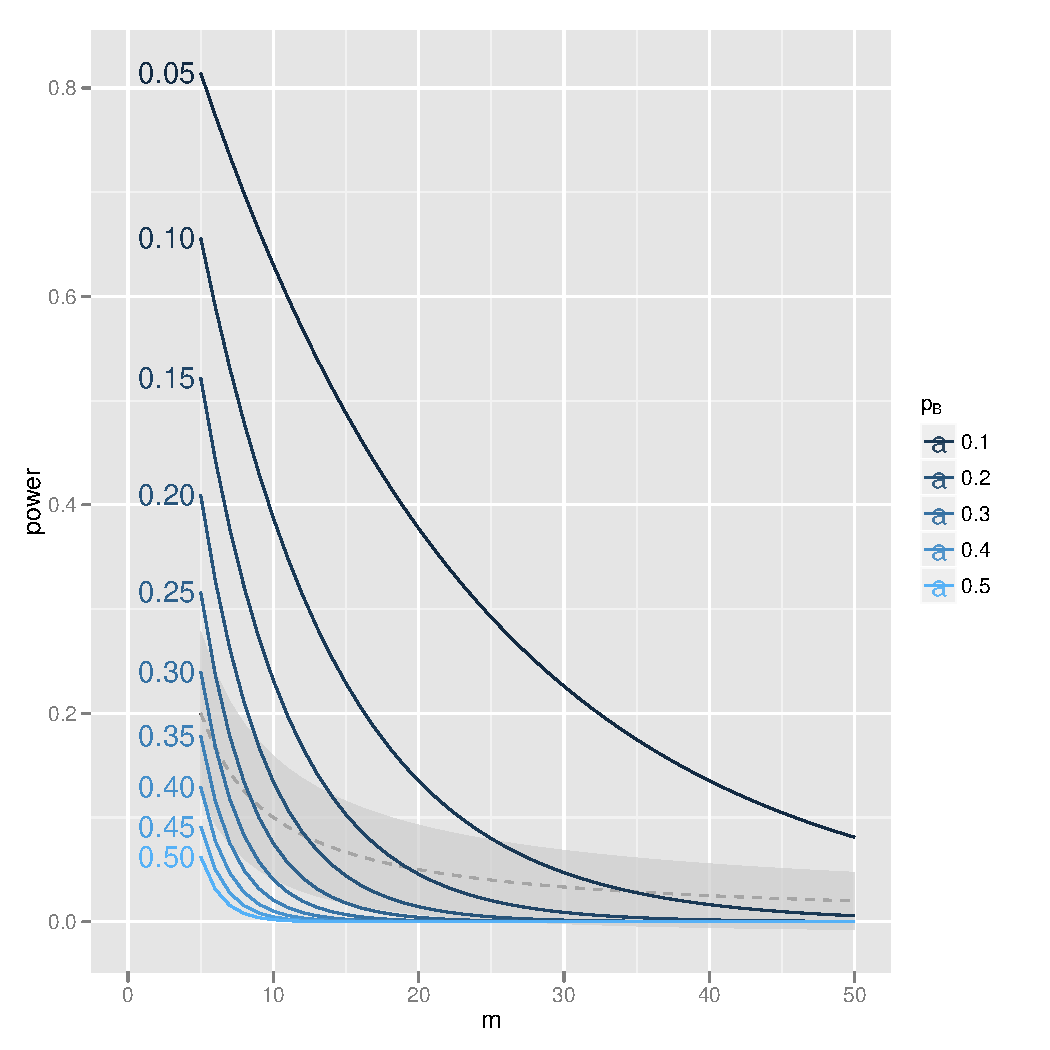
\includegraphics[width=3in]{images/powerplot.pdf} 
   \caption{Probability that the data plot has the smallest probability in a lineup of size $m$. With increasing $p$-value the probability drops -- when it reaches $1/m$ a horizontal line is drawn to emphasize insufficient sensitivity of the test due to the lineup size. 
   %Comparison of probabilities to pick the actual data plot for different size lineups, $m$, and different values for data plot strength, $p_D$. The dashed  line, and grey 95\% pointwise confidence band, shows the probability of picking the data plot, by chance, if $H_0$ is true. }
}
   \label{fig:pval_power}
\end{figure}

%Now assume that the same lineup plot is evaluated by $K$ independent observers. %W.l.o.g.\green{Can we get rid of cliches like WLOG?} 
%Let the last plot be the data plot and plots 1 through $m-1$ the null plots. Let $n_i$ be the number of observers who picked plot $i$ as the plot with the structure least consistent with the null hypothesis, corresponding to random variable $N_i$.  Then  $(N_1, N_2, ..., N_m) \sim$ Mult$_{\pi_1, ..., \pi_m}$ with $\sum_i \pi_i = 1$ and $\sum_{k=1}^{m} n_k = K$. We can estimate $\pi_i$ as $\widehat{\pi_i} = n_i/K$. 
%
%For the distribution of $N_m$, %the number of times out of $K$ that observers picked the last plot to show the structure least consistent with the null hypothesis, 
%we get
%\[
%N_m\sim \left \{ 
%\begin{array}{ll}
%B_{K, \hh{E\left[ (1 - p_D)^{m-1}\right]}} & \text { under } H_1\\
%B_{K, 1/m} & \text { under } H_0
%\end{array}
%\right .
%\]
%
%By matching the expected values, we therefore get an expression  for the $p$-value $p_D$ in the data 
%%under $H_1$  %% no such thing aas $p$-value under H_1 - even though it's just an unfortunate choice of word.
%as:
%\begin{equation}\label{eqn:power_estimate}
%%{E[p_D]} = 1- \left(\frac{E[N_m]}{K}\right)^{1/(m-1)}.
%\hh{1 - E[N_m]/K = (m-1)E[p_D] + O(E[p_D^2])}
%\end{equation}
%
%Note that the left hand side in Equation \ref{eqn:power_estimate} is independent of the parameter $\theta$, but just based on the lineup evaluation by independent observers. While this allows us to compute this value independently of the parametric setting, it also means that observers might pick out the data plot for a reason not related to the value of $\theta$. 
%\hh{Also note, that this equation yields an estimate of $p_D$ that is bounded by $1/(m-1)$. We should therefore not make the decision of significance depend on this estimate, but only use this equation after the fact. 
%Both of these topics are further highlighted in the application section.}

%Picking out the data plot is still a measure of how different the data plot is compared to the null plots, and therefore is a test statistic of the visual test.

%This allows us to compute this value independently of the parametric setting. We therefore define the {\it signal strength} of a  visual test as the following:
%
%\begin{dfn} \label{dfn:signal}
%The {\it signal strength} $\sigma_T$ of a visual test is defined as the probability to identify the data plot.
%\end{dfn}
%
%In a lineup of size $m$, evaluated by $K$ independent observers,  we can estimate the signal strength of the test as
%\[
%\sigma_T^{m-1} = \frac{n_m}{K}.
%\]
%
%In a parametric setting, signal strength of a test coincides with the power of the test.



%Theoretical power for the regression parameters is derived in the next section.
%\subsection{Estimating Power from Lineups}
%
%We estimate the empirical power from responses on a specific lineup plot  generated with known values of sample size ($n$), variance ($\sigma^2$) and regression parameter ($\beta$) in model \ref{multi}. Suppose, we have responses from $K$ independent observers with $u$ identifications of the actual plot. This gives an estimated power of
%\begin{equation}\label{power_est} Power(\beta)=\frac{u}{K} \hspace{1cm} 0 \le u \le K \end{equation}


%From model \ref{eqn:mixed} we obtain %$\pi=Pr(Y=1|X_1, X_2, ..., X_p)$, 
%the power of the underlying testing procedure as a population average %by ignoring the random effect part. 
%%Thus we have the overall probability of success ($\pi$ or power) 
%for specified sample size ($n$) and  variance ($\sigma$)  as 
%
%\begin{equation}\label{eqn:power} 
%Power(\beta) = \pi=Pr(Y=1|\beta, n, \sigma) 
%\end{equation}
%
%The main covariate factors that determine the power of the test are sample size ($n$), $\sigma$ and the parameter $\beta$. combining these we obtain one single covariate effect denoted by $E$ and defined as $E = \beta/ \sigma*\sqrt{n}$. Using equation \eqref{eqn:mixed}, we then have the power as
%
%\begin{equation}\label{eqn:effect} 
%Power(E) = \pi=Pr(Y=1| E) 
%\end{equation}

\section{Application to Linear Models} \label{sec:regression}

To make these concepts more concrete consider how this would operate in the linear models setting. Consider a linear regression model 
\begin{equation}\label{multi} Y_i = \beta_0 + \beta_1 X_{i1} + \beta_1 X_{i2} + \beta_3 X_{i1}X_{i2} + ... + \epsilon_i 
\end{equation}
where $\epsilon_i \stackrel{iid}{ \sim } N(0,\sigma^2)$, $i=1,2, .., n$. The covariates ($X_j, j=1,..,p$) can be continuous or discrete.

In this setting, there are many established graphics that are used to evaluate and diagnose the fit of a regression model (e.g. \citet{cook:99}). Table \ref{tbl:stat_multiple} lists several common hypotheses related to the regression setting, and commonly used statistical plots that might be used as corresponding visual test statistics.
%These plots should be familiar, because they are all in common use. 
For example, to examine the effect of variable $X_j$ on $Y$, we would plot $Y$ against $X_j$ (cases 1-4). To assess whether the linear assumption is appropriate we would draw a plot of residuals against fitted values (case 5). For the purposes of comparing visual against conventional inference, we focus on cases 2 and 3, with a continuous and categorical explanatory variable respectively. 

%Note that some charts can be associated with several different testing situations. In our paper, we pick the examples for situation 2 and 3 as candidates.

\begin{table*}[hbtp] 
\caption{Visual test statistics for testing hypotheses related to the model $Y_i = \beta_0 + \beta_1 X_{i1} + \beta_1 X_{i2} + \beta_3 X_{i1}X_{i2} + ... + \epsilon_i  $ } 
\centering 
\begin{tabular}{m{0.5cm}m{3cm}m{2cm}m{3cm}m{5.5cm}} 
\hline\hline 
Case & Null Hypothesis & Statistic & Test Statistic & Description \\ [0.5ex] % inserts table %heading 
\hline 
1 & $H_0: \beta_0=0$ & Scatter plot & \begin{minipage}[t]{3cm}  \scalebox{0.4}{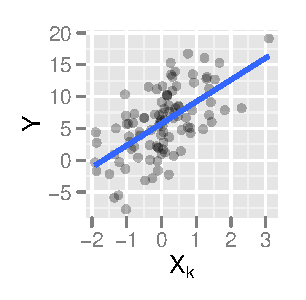
\includegraphics{stat_intercept.pdf}}\end{minipage} & Scatter plot with least square line overlaid. For lineup plot, we simulate data from fitted null model. \\ 
2 & $H_0: \beta_k=0$ & Residual plot & \begin{minipage}[t]{3cm}   \scalebox{0.4}{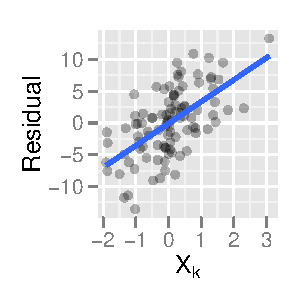
\includegraphics{stat_beta_k.pdf}}\end{minipage} & Residual vs $X_k$ plots. For lineup plot, we simulate data from normal with mean 0 variance $\hat{\sigma}^2$. \\ 
3 & $H_0: \beta_k=0$ (for categorical $X_k$) & Box plot & \begin{minipage}[t]{3cm} 	\scalebox{0.4}{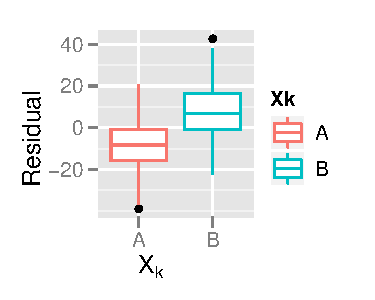
\includegraphics{stat_category.pdf}} \end{minipage} & Box plot of residuals grouped by category of $X_k$. For lineup plot, we simulate data from normal with mean 0 variance $\hat{\sigma}^2$. \\
4 & $H_0: \beta_k=0$ (interaction with categorical $X_k$) & Scatter plot & \begin{minipage}[t]{3cm}  \scalebox{0.4}{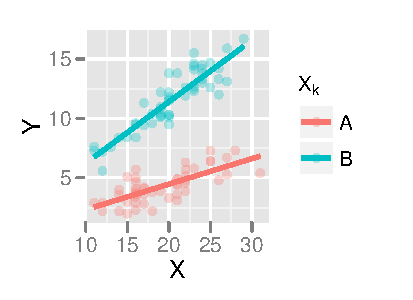
\includegraphics{stat_interection.pdf}}  \end{minipage} & Scatter plot with least square lines of each category overlaid. For lineup plot, we simulate data from fitted null model.\\[1ex] % [1ex] adds vertical space 
5 & $H_0: X$ Linear & Residual Plot & \begin{minipage}[t]{3cm}  	\scalebox{0.4}{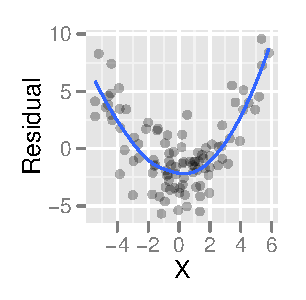
\includegraphics{stat_nonlinear.pdf}}  \end{minipage} & Residual vs predictor plots with loess smoother overlaid. For lineup plot, we simulate residual data from normal with mean 0 variance $\hat{\sigma}^2$. \\ 
6 & $H_0: \sigma^2=\sigma^2_0$ & Box plot & \begin{minipage}[t]{3cm} \scalebox{0.4}{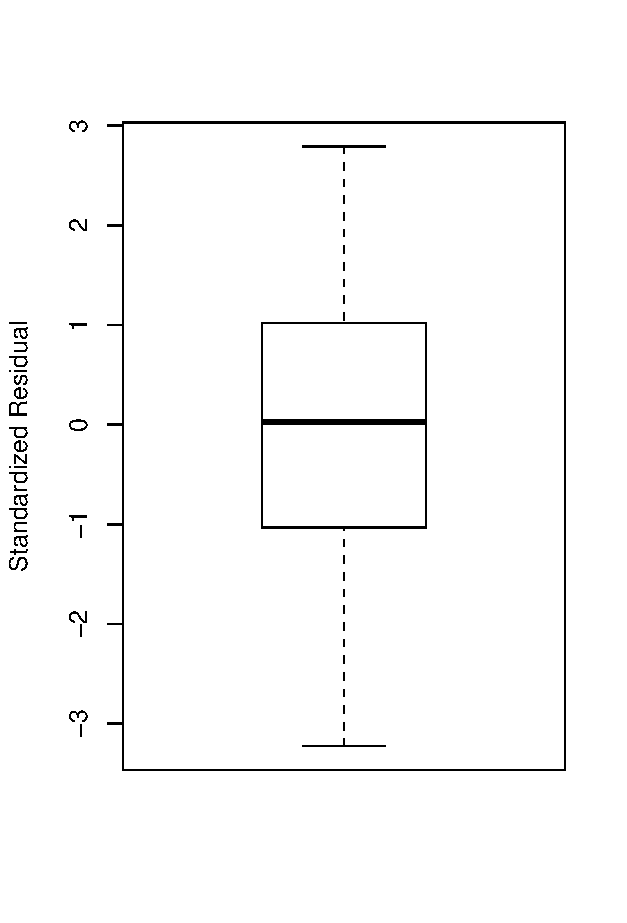
\includegraphics{stat_sigma_box.pdf}}\end{minipage} & Box plot of standardized residual divided by  $\sigma^2_0$. For lineup plot, we simulate data from standard normal. \\ 				
7 & $H_0: \rho_{X,Y|Z}=\rho$ & Scatter Plot & \begin{minipage}[t]{3cm}  	\scalebox{0.4}{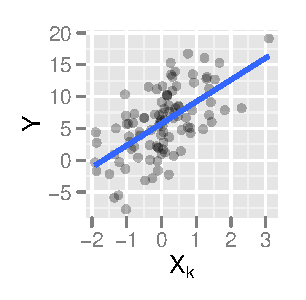
\includegraphics{stat_intercept.pdf}}  \end{minipage} & Scatter plot of Residuals obtained by fitting partial regression. For lineup plot, we simulate data (mean 0 and variance 1) with specific correlation $\rho$. \\ 
8 & $H_0:$ Model Fits & Histogram & \begin{minipage}[t]{3cm}  \scalebox{0.4}{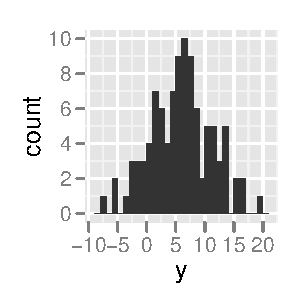
\includegraphics{stat_goodness_simple.pdf}}  \end{minipage} & Histogram of the response data. For lineup plot, we simulate data from fitted model. \\[1ex] % [1ex] adds vertical space 
9 & Special case $p=1$ $H_0: \rho_{X,Y} =\rho$ & Scatter plot & \begin{minipage}[t]{3cm}  \scalebox{0.4}{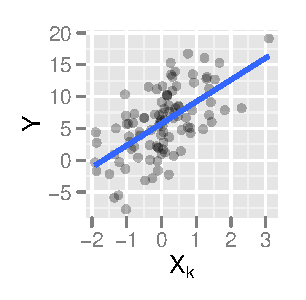
\includegraphics{stat_intercept.pdf}}  \end{minipage} & Scatter plot with least square line overlaid For lineup plot, we simulate data with correlation $\rho$.\\			
\hline 
\end{tabular} 
\label{tbl:stat_multiple} 
\end{table*} 

Suppose $X_k$ is a categorical variable with two levels, and we test the hypothesis $H_0:\beta_k=0$ vs $H_1: \beta_k \ne 0$. If the responses for the two levels of the categorical variable $X_k$ in the model are different, the  residuals from fitting the null model should show a significant difference between the two groups. For a visual test, we draw boxplots of the residuals conditioned on the two levels of $X_k$. If $\beta_k\ne 0$ the boxplots should show a vertical displacement. 

%A lineup including the test statistic  for a binary $X_k$ is shown in Figure \ref{fig:test_category}. The 19 null plots are generated  by simulating residuals from $N(0,\hat{\sigma}^2)$. The test statistic, the plot containing the actual data, is randomly placed among these null plots. If the test statistic is identifiable the null hypothesis is rejected. % with a $p$-value of at most 0.05.

%\subsection{Expected power}

% Di: This is specific for the regression model
%Consider the hypothesis test $H_0: \beta_k=0$ against $H_1: \beta_k \ne 0$ in model \ref{multi}.
%%Now consider estimating the power of the visual test. 
%%Suppose $F_{|t|}(.)$ is the distribution function of an absolute value of $t$. For the regression slope parameter $\beta$ suppose the associated test statistic in conventional test be $t_{obs}$ with $p$-value $p_D$. By definition we have 
%%
%%$$p_D=Pr(|t| \ge t_{obs}| H_0)=1-F_{|t|}(t_{obs}) \Rightarrow |t_{obs}|=F_{|t|}^{-1}(1-p_D)$$
%%
%%\red{HH: the following paragraph should probably move up, but I'm not sure how to change it appropriately. Mahbub, could you take care of that?}
%%Now suppose $F_{|t|}(.;\delta)$ denotes the distribution function of an absolute value of $t$ distribution with non-centrality parameter $\delta$. Thus the distribution function of $p-value$ be  
%%\begin{eqnarray}\label{dist_p}
%%F{p_D}(p) &=& Pr(p_D \le p)=1-Pr(1-p_D \le 1-p) \nonumber \\
%%  &=& 1-Pr(F_{|t|}^{-1}(1-p_D) \le F_{|t|}^{-1}(1-p) ) \nonumber \\
%%  &=& 1-Pr(|t_{obs}| \le F_{|t|}^{-1}(1-p)) \nonumber \\
%%  &=&\left\{ \begin{array}{ll}
%%          1-F_{|t|}( F_{|t|}^{-1}(1-p))=p &\mbox{ ; under $H_0$} \\
%%          1-F_{|t|}( F_{|t|}^{-1}(1-p); \delta) &\mbox{ ; under $H_1$} 
%%       \end{array} \right.     
%%\end{eqnarray}
%%
%%Thus the density of $p_D$ is Uniform(0,1)  under $H_0$. As noted by \cite{Ruppert:2007}, under $H_1$ the density $$f_{p_D}(p_D; \delta)= \frac{f_{|t|}(F_{|t|}^{-1}(1-p_D);\delta)}{f_{|t|}(F_{|t|}^{-1}(1-p_D))}$$ derived from equation \eqref{dist_p}  is a right skewed distribution.  
%In a lineup plot we simulate $m-1$ residual data sets from null model where each of these $m-1$ null data sets produces a corresponding $p$-value $p_{0,i}$ and $p_{0,i} \sim \text{Uniform}(0,1)$ for $i = 1, ..., m-1$. Suppose  $p_0=\min_i(p_{0,i})$. Thus $p_0 \sim \text{Beta}(1,m-1)$. 

The conventional test in this scenario uses $T= \hat{\beta_k}/ se(\hat{\beta_k})$ and rejects the null hypothesis, if $T$ is extreme on the scale of a $t$ distribution with $n-p$ degrees of freedom.  It forms the benchmark upon which we evaluate the visual test. To calculate what we might expect for the power of the visual test, under perfect conditions, first assume that the observer is able to pick the plot with the smallest $p$-value from a lineup plot.  This leads to the decision to reject $H_0$ when $p_{D} < p_0$, where $p_{D}$ is the conventional $p$-value as details given in Lemma \ref{lemma}. Thus the expected power of the visual test in this scenario is

\begin{equation}\label{power_exp} 
   Power(\beta)=Pr(p_{D} < p_0)  \quad \text{for}  \quad \beta \ne 0
\end{equation}
Figure \ref{fig:power_expected} shows the power of the conventional test in comparison to the expected power of the visual test obtained from Equation \ref{power_exp}. Notice that the expected power of the visual test is %almost as good as 
close to the power of the conventional test. 


%Theorem \ref{thm:power} helps to compute the expected power of visual inference.
%\begin{thm}\label{thm:power}
% equation \eqref{power_exp}  yields expected power of visual inference as Power($\beta$) = $E(1-p_D)^{m-1}$ .
%\end{thm}
% 
%{ \em proof}
%
%Since $p_0 \sim \text{Beta}(1,m-1)$,  for $t \in (0,1)$ we have the distribution function of $p_0$ be
%\begin{eqnarray*}
%F{p_0}(t) &=& (m-1) \int_0^t{(1-p_0)^{(m-2)}dp_0} \\
%  &=&  -(m-1) \int_1^{1-t}{x^{(m-2)}dx}\\
%  &=& \left[ x^{m-1}\right]^1_{1-t}\\
%  &=&1-(1-t)^{m-1} \rightarrow 1 \quad \text{as} \quad m \rightarrow \infty
%\end{eqnarray*}
%
%% verified this computation from http://www.wolframalpha.com using command int (m-1)*(1-p)^(m-2) dp, p=0,t
%
%Thus expected power in equation \eqref{power_exp} be
%\begin{eqnarray*}
% Pr(p_{B} < p_0) &=& 1- Pr( p_0 \le p_{B} ) \\
%  &=& 1- \int_{0}^{1}{Pr( p_0 \le p_{B} |p_{B} =t) f_{p_{B} }(t)dt } \\
%  &=& 1-  \int_{0}^{1}{F{p_0}(t) f_{p_{B} }(t)dt } \\
%  &=& E(1-p_D)^{m-1}   \\
%%  & \rightarrow &1-  \int_{0}^{1}{ f_{p_{B} }(t)dt }  = F_{p_D}(0) \quad \text{as} \quad m \rightarrow \infty
%\end{eqnarray*}
%
%
\begin{figure}[hbtp]
   \centering
       \scalebox{.6}{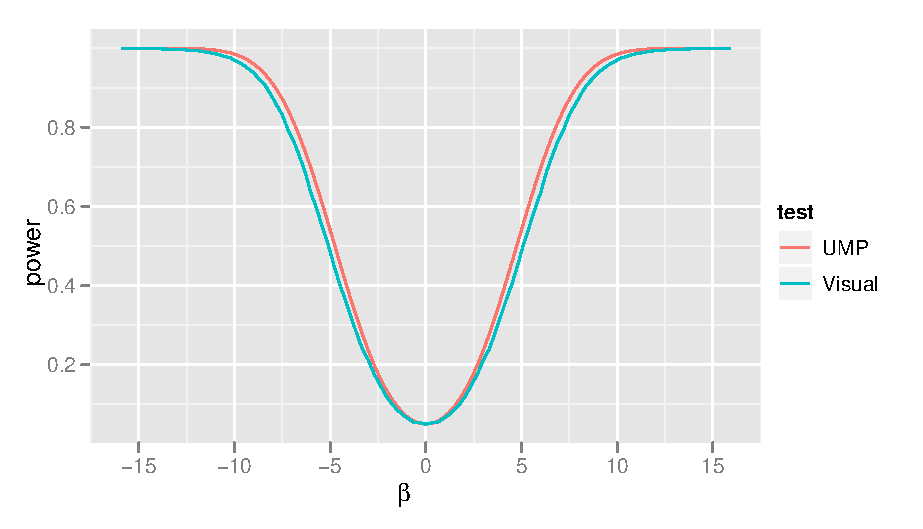
\includegraphics{power_expected.pdf}}
       \caption{Expected power of visual test  and the power of conventional test for sample size $n =100$, $\sigma = 12$ and $m$=20. }
       \label{fig:power_expected}
\end{figure}

% \pagebreak

% -------- Heike's writeup added here

%\subsection{Some Power Considerations}


%\subsection{Expected number of choices}
%Since $X$ has a binomial distribution, we can have a look at the number of plots among the null plots that we would expect to be picked over the data plot:
%\[
%E[X] = (m-1)(1-E[p_D]).
%\]
%With an increase of the lineup size $m$ the number of null plots with a potentially stronger signal than the data plot grows linearly.
%This should allow us to infer some of the signal strength $p_D$ as
%\begin{equation} \label{plot_signal}
%E[p_D] = 1 - E[X]/(m-1),
%\end{equation}
%i.e. by averaging over the number of plots with  a stronger signal than the data plot we can evaluate signal strength of the plot even in the case where the data plot is not being picked by the observer.
%

\section{Human Subjects Experiments with Simulated Data} \label{sec:simulation}

Three experiments were conducted to evaluate the effectiveness of the lineup protocol relative to the equivalent test statistic used in the regression scenario. The first two are conventional settings where we would not expect the lineup protocol to do better than the conventional test, but we hope it to perform favorably. The third experiment is a scenario where assumptions required for the conventional test are violated, and we would expect the lineup protocol to outperform the conventional test. (Data and lineups used in the experiments are available in the supplementary material.)

After many small pilot studies with local personnel, it was clear that some care was needed to set up the human subjects experiments. It was best for a observer or a subject to see a block of 10 lineups with varying difficulty, with a reasonable number of ``easy'' lineups. The explanations about each experiment (below) includes an explanation of how the lineups were sampled and provided to the subjects, for each of the three experiments.

Participants for all the experiments were recruited through Amazon's online web service, Mechanical Turk  \citep{turk}. A summary of the data obtained for all three experiments are shown in Table \ref{tbl:summary}. Participants were asked to select the plot they think best matched the question given, provide a reason for their choice, and say how confident they are in their choice. Gender, age, education and geographic location of each participant are also collected. %The data was collected through the web. 
For each of the experiments one of the lineups was used as a test plot (easy plot) which everyone should get correct, so that a measure of the quality of the subjects effort could be made. 

Note that no participant was shown the same lineup twice.
%\green{Something probably needs to be said about subjects who do multiple tests, what checks are done.} \blue{We do have some data where we notice multiple responses for a lineup by a subject. This happens when subject accidentally use browser's ``back'' button and same data is saved twice. We made sure in the data cleaning process that we do not include more than one response on a lineup by a subject. For this we only keep the very first response.}

\subsection{Discrete covariate}\label{sec:category}

The experiment is designed to study the ability of human subjects to detect the effect of a single categorical variable $X_2$ (corresponding to parameter $\beta_2$) in a two variable ($p=2$) regression model (Equation \ref{multi}). Data is simulated a range of values of $\beta_2~ (=0, 1, 3, 5, 7, 8, 10, 16)$, two different sample sizes ($n=100, 300$) and two standard deviations of the error ($\sigma=5, 12$). The range of $\beta_2$ values was chosen so that estimates of the power would produce reasonably continuous power curves, comparable to that calculated for the theoretical conventional test. Values were fixed for other regression parameters, $\beta_0 = 5$,  $\beta_1=15$, and the values for $X_1$ were randomly generated from a Poisson $(\lambda=30)$ distribution, which is almost Gaussian. Data sets were generated with parameter values shown in Table \ref{tbl:experiment_params}. Three replicates at each level were generated. These produced 60 different ``actual data sets'', and thus, 60 different lineups. To produce the lineups, the null model was fit to each actual data set, to obtain residuals and parameter estimates. The actual data plot was generated by making  side-by-side boxplots of the residuals (Table \ref{tbl:stat_multiple}, case 3). The 19 null data sets were generated by simulating from  $N(0, {\hat{\sigma}}^2)$, and  plotted in the same way. The actual data plot was randomly placed among these null data plots to produce the lineup. Figure \ref{fig:test_category} is an example of one of these lineups. The actual data plot is number 11 which was generated for $n$=300, $\beta_2$=15 and $\sigma$=12.  

%{\bf Steps to obtain lineup}
%\begin{enumerate}
%	\item For a given parameter setting obtain actual data set
%	\item Fit the null model to the actual data and obtain residuals and other parameter estimates ($\hat{\beta}$ and $\hat{\sigma}$)
%	\item Generate actual data plot using the procedure as described in table \ref{tbl:stat_multiple}
%	\item Generate 19 null (residual) data sets from $N(0, {\hat{\sigma}}^2$) and obtain 19 null plots
%	\item Finally randomly place 19 null plots and one actual plot in a layout (4X5) to get a lineup 
%\end{enumerate}

The number of evaluations required for each lineup to provide reasonable estimates of the power is determined by the variance of the estimated power. Suppose $\gamma$ denotes the conventional test power for each parameter combination shown in Table \ref{tbl:experiment_params}. Since the expected power of visual inference is very close to the power of conventional test (Figure \ref{fig:power_expected}) the proportion of successful evaluations of lineups should give a rough estimate for  $\gamma$. 
For a given proportion $\gamma$ it is desired to have a margin of error (ME) less than or equal to 0.05. Thus we have $ME =1.96 \sqrt{ \gamma(1-\gamma) / n_{\gamma} } \le 0.05$ which gives us the estimation of minimum number of evaluations $$n_{\gamma} \geq \frac{\gamma(1-\gamma)}{(0.05/1.96)^2}.$$  
% \hh{we're not even close to $n_\gamma$ with ten lineups .... we need more in the order of 400. Let's not emphasize this so much.}

Each subject viewed at least 10 lineups with the option to evaluate more.
%and we allowed them to provide more evaluations if they wanted. 
Depending on the parameter combinations we group the lineups in different difficulty levels  as easy, medium, hard and mixed (actual numbers are given in the supplementary material). For each difficulty level a specific number of lineups was randomly picked  for evaluation. This number is chosen so that total number of evaluations for each lineup for that group exceed the threshold $n_{\gamma}$. To satisfy this plan we needed to recruit at least 300 subjects. 

\begin{table}[hbtp]
\caption{Combination of parameter values, $\beta_2$,  $n$ and $\sigma$, used for each of the simulation experiments.} % title name of the table
\centering
\scalebox{.9}{
\begin{tabular}{c c c c c}
% creating 10 columns
\hline\hline

% inserting double-line
& & \multicolumn{3}{c}{Slope ($\beta$)} \\
 \cline{3-5}

Sample size  & Error SD  &  \multicolumn{1}{c} {Experiment 1}  & \multicolumn{1}{c} {Experiment 2}  & \multicolumn{1}{c} {Experiment 3} \\
 ($n$) &   ($\sigma$) & Discrete covariate & Continuous covariate & Contaminated data 
\\ [0.5ex]
\hline
% inserts single-line

% Entering 1st row
&  5 & 0, 1,  3, 5, 8  & 0.25, 0.75, 1.25, 1.75, 2.75 & 0.1, 0.4, 0.75, 1.25, 1.5, 2.25\\[-1ex]
\raisebox{1.5ex}{100} &12
& 1, 3, 8, 10, 16  & 0.5, 1.5, 3.5, 4.5, 6 &\\[1ex]

% Entering 2rd row
&  5 & 0, 1, 2, 3, 5  & 0.1, 0.4, 0.7, 1, 1.5&\\[-1ex]
\raisebox{1.5ex}{300} & 12
& 1, 3, 5, 7, 10  & 0, 0.8, 1.75, 2.3, 3.5 &\\[1ex]
% [1ex] adds vertical space
\hline
% inserts single-line
\end{tabular}
}
\label{tbl:experiment_params}
\end{table} 

%For a given proportion $p$ we want to have margin of error (ME) to be 0.1. Thus we have $ME =1.96 \sqrt{ \frac 1 n p(1-p)} \le 0.05$ which gives us the estimation of minimum number of evaluations $$n_p \geq \frac{p(1-p)}{(0.05/1.96)^2}.$$ Now from the theoretical (UMP) power curve for each parameter combinations shown in Table \ref{tbl:experiment_params} we know the power(say $p$) and thus we can estimate the number of evaluations required for that specific combinations of parameter. We collect data such that each of the parameter combinations in the Table \ref{tbl:experiment_params} has approximately the estimated sample size that we calculated here.
 


%\green{Did you in fact bin like this???}\red{For each parameter combination a set of 1000 actual data are generated and their associated p-values were computed. This produces an empirical distribution of p-value under alternative hypothesis. Finally, three data sets that have 16th, 50th and 84th quantile of the p-values were taken. Similar procedure was used to generate 19 null plots based on the empirical distribution of p-value under null hypothesis}. For added control, to ensure a signal in the simulated actual data a blocking structure was used to filter data sets. A 1000 sets were generated for each parameter combination and the conventional $t$-statistic and $p$-value associated with $H_0: \beta_2=0$ were calculated. The 3 replicates were drawn from each of three blocks of $p$-values: (0.0-$q_{33}$), ($q_{33}$-$q_{66}$), ($q_{66}$-1) where $q_i$ is the $i$th percentile in the distribution of the $p$-values. Additional control was applied to the 19 null plots. Because the distribution of these $p$-values should follow a Uniform(0,1) distribution, data sets were binned on this range by $p$-value, and a data set was randomly selected from each bin.
  
\subsection{Continuous covariate} 

This experiment is very similar to the previous one, except that there is a single continuous covariate and no second covariate (Equation \ref{multi} with $p=1$), following the test in Table \ref{tbl:stat_multiple}, case 2. Data is simulated with two sample sizes ($n=100, 300$), two standard deviations of the error ($\sigma=5, 12$), a variety of slopes ($\beta$), as given in Table  \ref{tbl:experiment_params}. We arbitrarily fix $\beta_0 = 6$ and values for $X_1$ are simulated from $N(0,1)$. For each combination of parameters, three different actual data sets are produced, yielding a total of 65 lineups. For some parameter combinations we have more than three replications, because additional lineups were produced for values of the parameters that exhibited large variation in the initial data.

The actual data plot is generated by making a scatterplot of $Y$ vs $X_1$ with the least squares regression line overlaid. To produce the null plots in the lineup null data was simulated from $N(X \hat{\beta}, {\hat{\sigma}}^2$) and plotted using the same scatterplot method as the actual data. 
To select 10 lineups for a subject, each combination of sample size ($n$) and error SD ($\sigma$) is given a difficulty value based on the slope ($\beta$) parameters. For the smallest slopes the difficulty is 4 (hardest) and for the largest slopes the difficulty is 0 (easiest). 
Figure \ref{fig:test_continuous} shows an example lineup for this experiment from difficulty level 4.  This lineup is generated using sample size ($n$)=100, slope($\beta$)=1.25 and and error SD($\sigma$)=5. The actual data plot location is 11. 

For each combination of sample size and standard deviation, the subject sees a randomly selected lineup of each difficulty level, all the slopes, giving 5 lineups. Another four lineups are chosen from a second choice of sample size and standard deviation, with difficulty levels 0-3, and the last lineup shown was a randomly selected lineup with difficulty 0. The order that the lineups are shown to participants is randomized. Each subject saw a substantial number of difficult lineups. 

%\hh{While this allows us a better estimation for the power in small slopes, }
%%The intention was noble, to get a better handle on the power of the lineups for small slopes, 
%but practically this made the study very tiring for the participants. %It would be better to provide the subjects with a larger selection of easier lineups and just a few difficult ones. 
%\green{perhaps should go into so much detail about this, or keep this for the conclusions section.}  

%{\bf Steps to obtain lineup}
%\begin{enumerate}
%	\item For a given parameter setting obtain actual data set
%	\item Fit the null model to the actual data and obtain residuals and other parameter estimates ($\hat{\beta}$ and $\hat{\sigma}$)
%	\item Generate actual data plot (a scatter plot of $Y$ vs $X_1$ a least square line overlaid)
%	\item Generate 19 null data sets from $N(X \hat{\beta}, {\hat{\sigma}}^2$) and obtain 19 null plots
%	\item Finally randomly place 19 null plots and one actual plot in a layout (4X5) to get a lineup 
%\end{enumerate}

%\green{Fill in details of lineups, probably need a figure with an example lineup, and how lineups were assigned to subjects.}

%{\bf Presenting lineups for evaluation} Each subject got at least 10 lineups for evaluation. For each combination of sample size ($n$) and error SD ($\sigma$) we define the difficulty of the lineup based on the five slope ($\beta$) parameters we choose as shown in Table \ref{tbl:experiment_params}. For the smallest slope parameter the difficulty is 0 and for the largest parameter the difficulty is 4. The 10 lineups are chosen as follows;

%\begin{enumerate}
%	\item For one combination of  sample size ($n$) and error SD ($\sigma$) randomly select five lineups with one from each difficulty level
%	\item For another combination of sample size ($n$) and error SD ($\sigma$) select four lineups with one from each difficulty level 0 through 3
%	\item Finally select another lineup with difficulty level 0
%\end{enumerate}


\begin{figure}[p]
%\begin{figurehere}
   \centering
       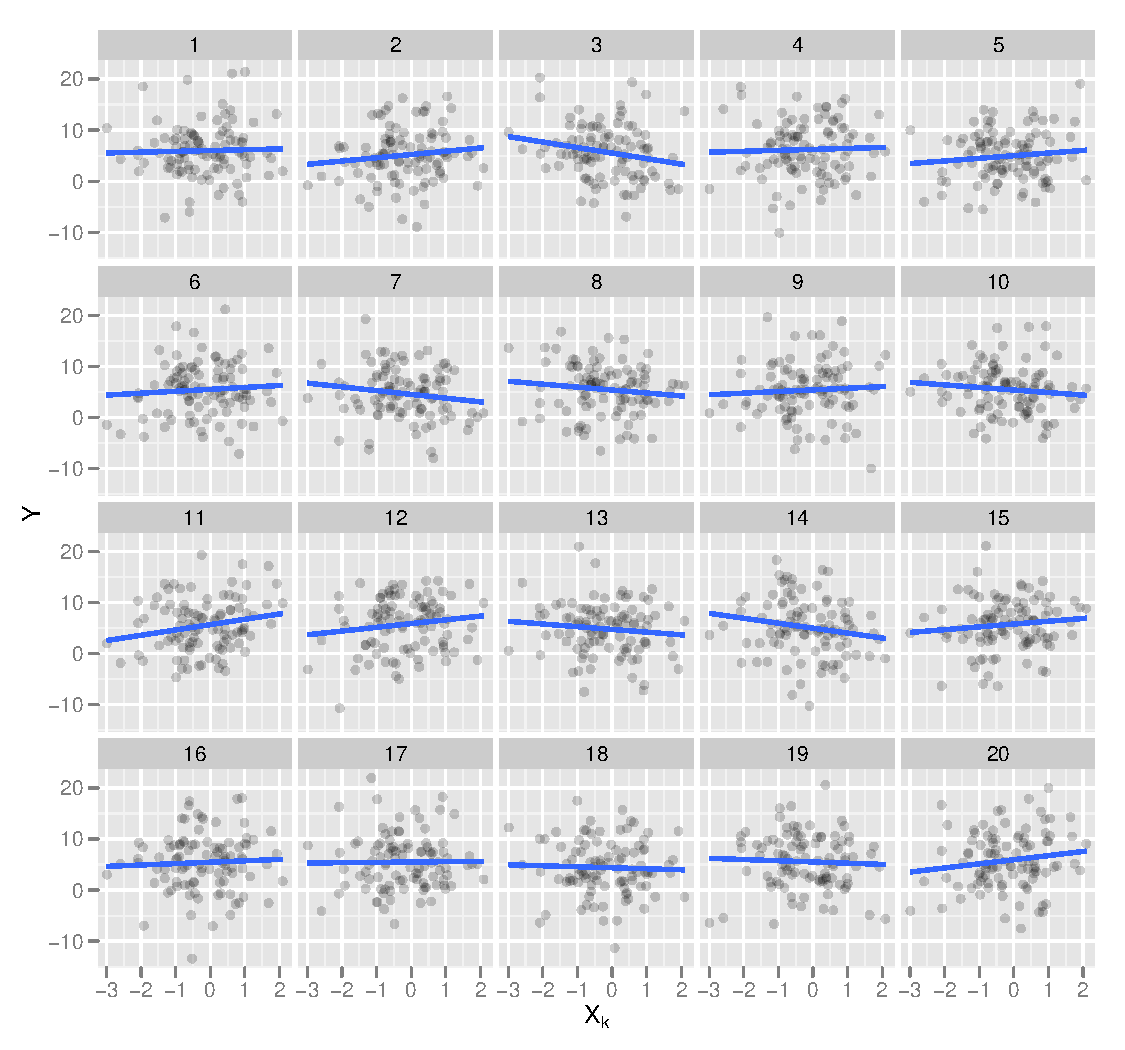
\includegraphics[width=0.95\textwidth]{lineup_continuous.pdf}
       \caption{Lineup plot ($m=20$) using scatter plots for testing $H_0: \beta_k=0$ where covariate $X_k$ is continuous. One of these plots is the plot of the actual data, and the remaining are null plots, produced by simulating data from a null model that assumes $H_0$ is true. Which plot is the most different from the others, in the sense that there is the steepest slope?}
       \label{fig:test_continuous}
\end{figure}

\subsection{Contaminated data}

The first two simulation experiments use data generated under a normal error model, satisfying the conditions for conventional test procedures. In these situations there exists a test, and there would, in general, be no need to use visual inference. The simulation is conducted with the hopes that the visual test procedure,  will at least compare favorably with the conventional test -- without any ambition of performing equally well.
 This third simulation is closer to the mark for the purpose of visual inference. The assumptions for the conventional test are violated, by contaminating the data. The contamination makes the estimated slopes effectively 0, yet the true value of slope parameter is not.  The data is generated from the following model:

\[
  Y_i = \left\{
  \begin{array}{l l}
    \alpha+\beta X_i + \epsilon_i  & \quad  X_i \sim N(0,1) \quad  i =1,...,n\\
    \lambda+ \eta_i & \quad X_i \sim N(\mu,1/3) \quad  i=1, ...,n_c\\
  \end{array} \right.
\]
where $\epsilon_i \stackrel{iid}\sim N(0,\sigma)$, $\eta_i \stackrel{iid}\sim N(0,\sigma/3)$ and $\mu = -1.75$. $n_c$ is the size of thecontaminated data. For the experiment we consider $n=100$ and $n_c=15$ producing actual data with $115$ points. Further, $\alpha=0$, $\lambda=10$, and $\sigma$ is chosen to be approximately 3.5, so that error standard deviation across both groups of the data is $5$. %Figure \ref{fig:cont_dat} shows an example of contaminated data, generated by this model for $\beta=5$.  
A linear model (Equation \ref{multi} with $p=1$  and intercept $\beta_0=0$) is fit to the contaminated data. This experiment  follows the test in Table \ref{tbl:stat_multiple}, case 2. The actual data plot shows a scatterplot of the residuals vs $X_1$, and the null  plots are scatterplots of null data generated by plotting simulated residuals from $N(0, {\hat{\sigma}}^2$)  against $X_1$. 

Experiment three consists of a total of 30 lineups, made up of five replicates for each of the six slopes as shown in Table \ref{tbl:experiment_params}. We use the slope directly as a measure of difficulty, with difficulty = 0 for the largest slope and difficulty = 5 for the smallest slope.  Subjects were exposed to a total of ten lineups, with two lineups from each of the difficulty levels 0 through 3, and one  lineup each from levels 4 and 5.

%{\bf Steps to obtain lineup}
%\begin{enumerate}
%	\item For a given parameter setting obtain actual data set
%	\item Fit the null model to the actual data and obtain residuals and other parameter estimates ($\hat{\beta}$ and $\hat{\sigma}$)
%	\item Generate actual data plot (a scatter plot of Residual vs $X_1$)
%	\item Generate 19 null residual data sets from $N(0, {\hat{\sigma}}^2$) and obtain 19 null plots
%	\item Finally randomly place 19 null plots and one actual plot in a layout (4X5) to get a lineup 
%\end{enumerate}

An example lineup for slope $\beta=0.4$ is shown in Figure \ref{fig:test_contaminated}.  Can you pick which plot is different? %Plot 7 is the actual data plot. 

%\begin{figure}[hbt]
%\begin{figurehere}
%   \centering
%       \scalebox{0.6}{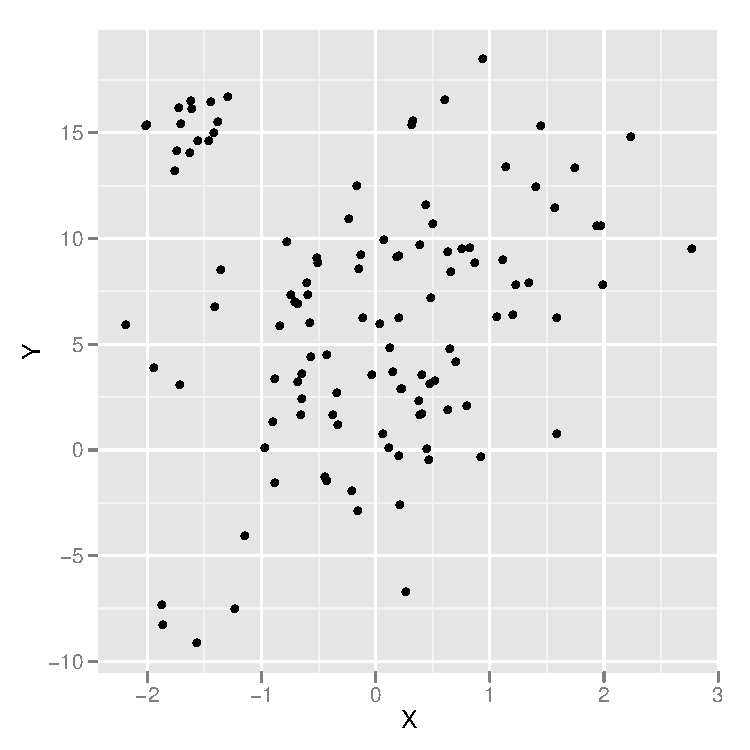
\includegraphics{contaminated_data.pdf}}
%       \caption{Scatterplot of a simulated contaminated data set generated such that a simple linear model produce a slope almost negligible, ie, if we fit model (Equation \ref{multi}) with $p=1$  to this data, the resulting estimate of $\beta_1$ would not be statistically significant. The conventional t-test $p$-value for the slope is 0.67 for this data set but visually we can see a convincing evidence of positive slope. 
%}
%       \label{fig:cont_dat}
%\end{figure}

\begin{figure}[p]
%\begin{figurehere}
   \centering
       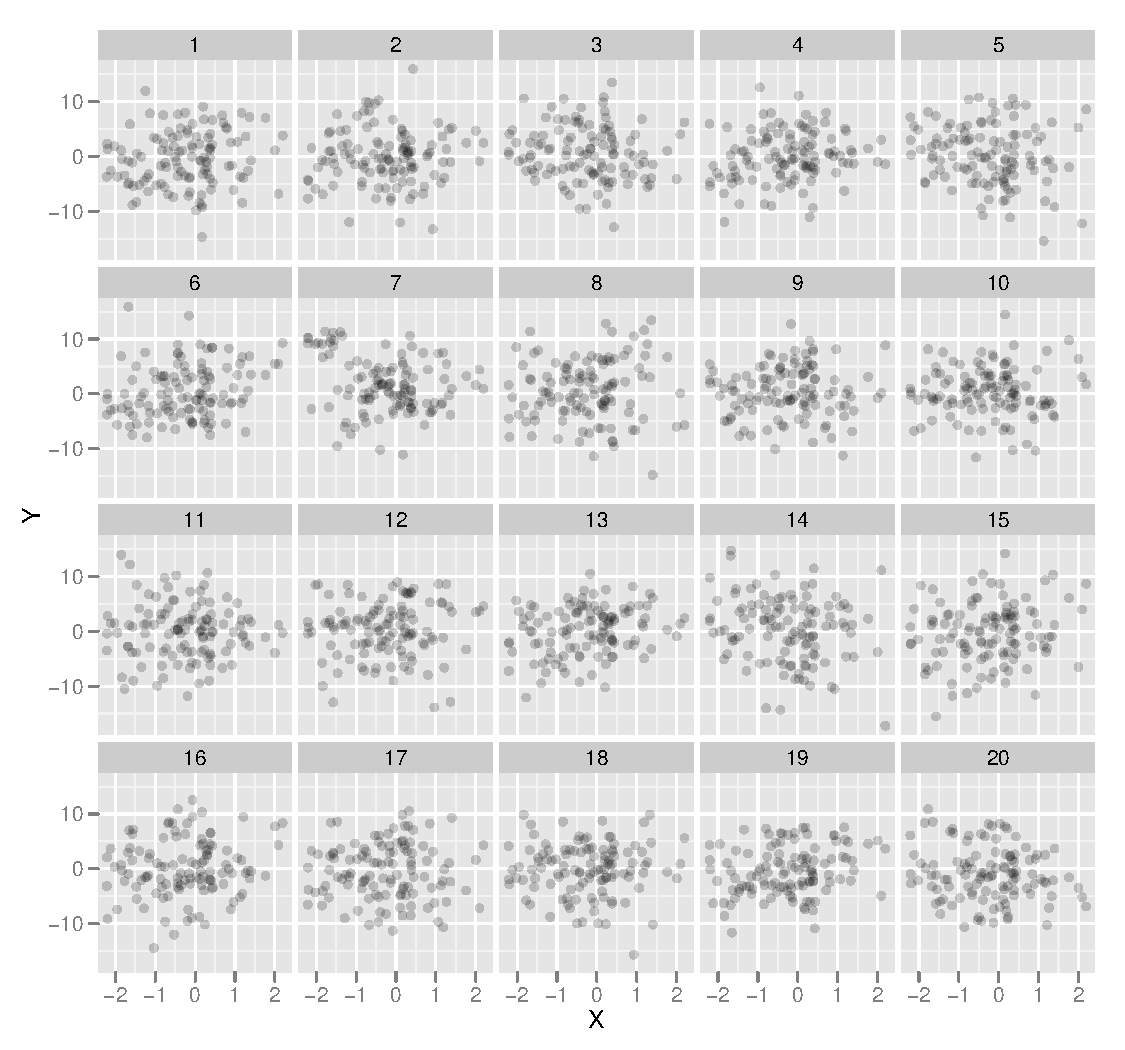
\includegraphics[width=0.95\textwidth]{lineup_contaminated.pdf}
       \caption{Lineup plot ($m=20$) using scatter plots for testing $H_0: \beta_k=0$ where covariate $X_k$ is continuous but the inclusion of some contamination with the data spoils the normality assumption of error structure. One of these plots is the plot of the actual data, and the remaining are null plots, produced by simulating data from a null model that assumes $H_0$ is true. Which plot is the most different from the others, in the sense that there is the steepest slope?}
       \label{fig:test_contaminated}
\end{figure}

%\green{Fill in details of lineups, probably need a figure with an example lineup, and how lineups were assigned to subjects. Show a sample lineup, probably the most difficult, instead of the single plot.}


%\begin{figure*}[hbtp]
%   \centering
%       \scalebox{0.6}{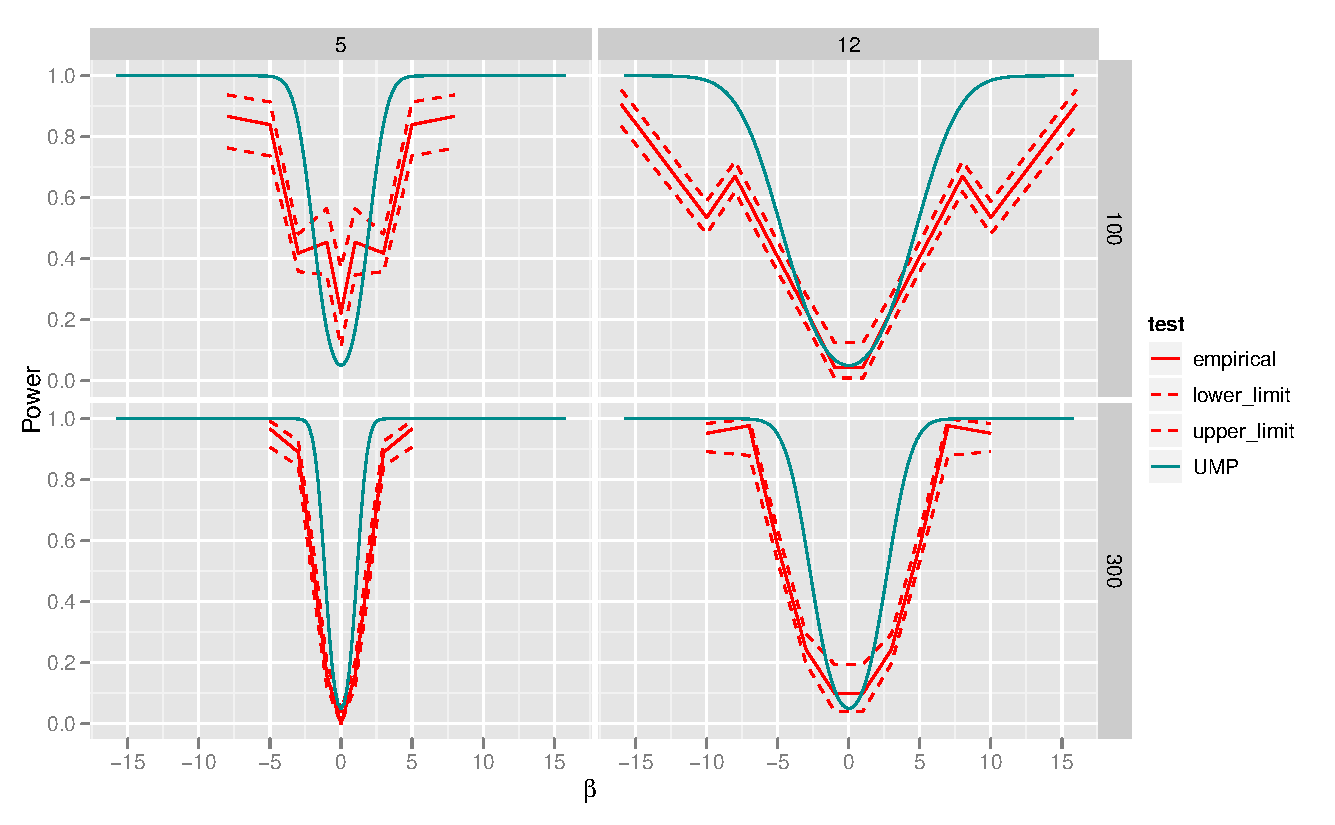
\includegraphics{power_observed.pdf}}
%       \caption{Observed power of visual test from equation \eqref{eqn:power_estimate} with pointwise 95\% confidence limits and the power of UMP test for sample size $n= 100,300$ and $\sigma = 12,5$ as per experiment 1.}
%       \label{fig:power_observed}
%\end{figure*}

%\begin{figure*}[hbtp]
%   \centering
%       \scalebox{0.7}{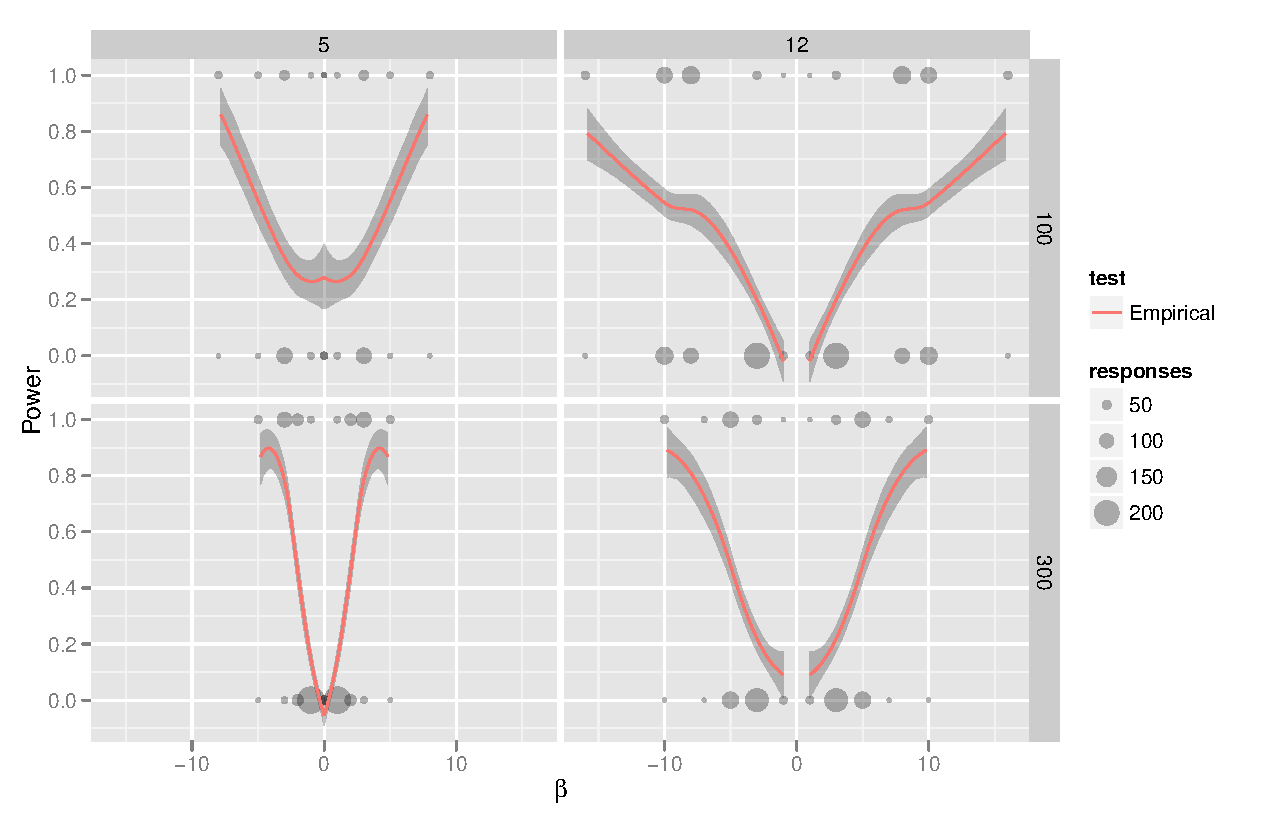
\includegraphics{power_loess_exp1.pdf}}
%       \caption{Observed power shown by loess smoother with simultaneous bootstrap confidence band and the power of UMP test for sample size $n= 100,300$ and $\sigma = 12,5$ as per experiment 1.}
%       \label{fig:power_loess1}
%\end{figure*}


%\begin{figure*}[hbtp]
%   \centering
%       \scalebox{0.7}{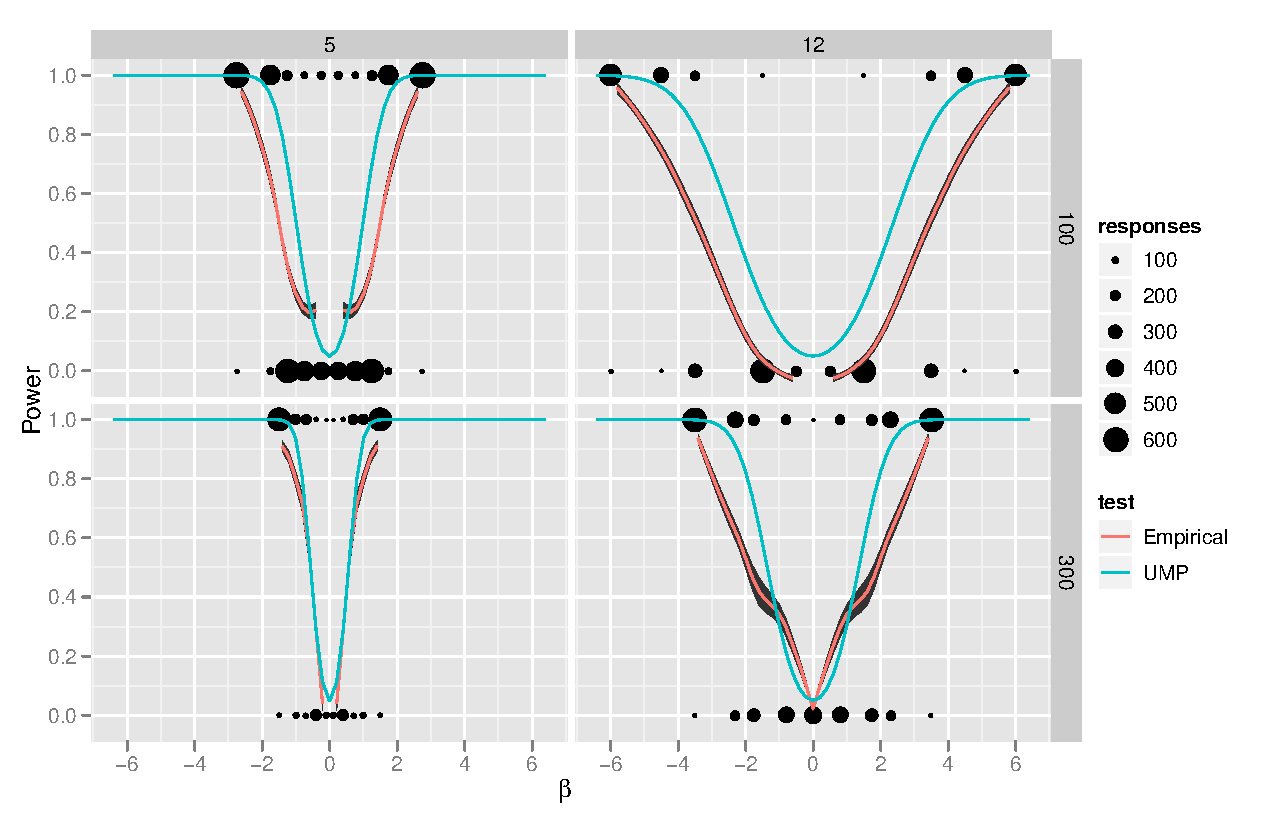
\includegraphics{power_loess_exp2.pdf}}
%       \caption{Observed power shown by loess smoother with simultaneous bootstrap confidence band and the power of UMP test for sample size $n= 100,300$ and $\sigma = 12,5$ as per experiment 2.}
%       \label{fig:power_loess2}
%\end{figure*}




%\begin{figure*}[hbtp]
%   \centering
%       \scalebox{0.7}{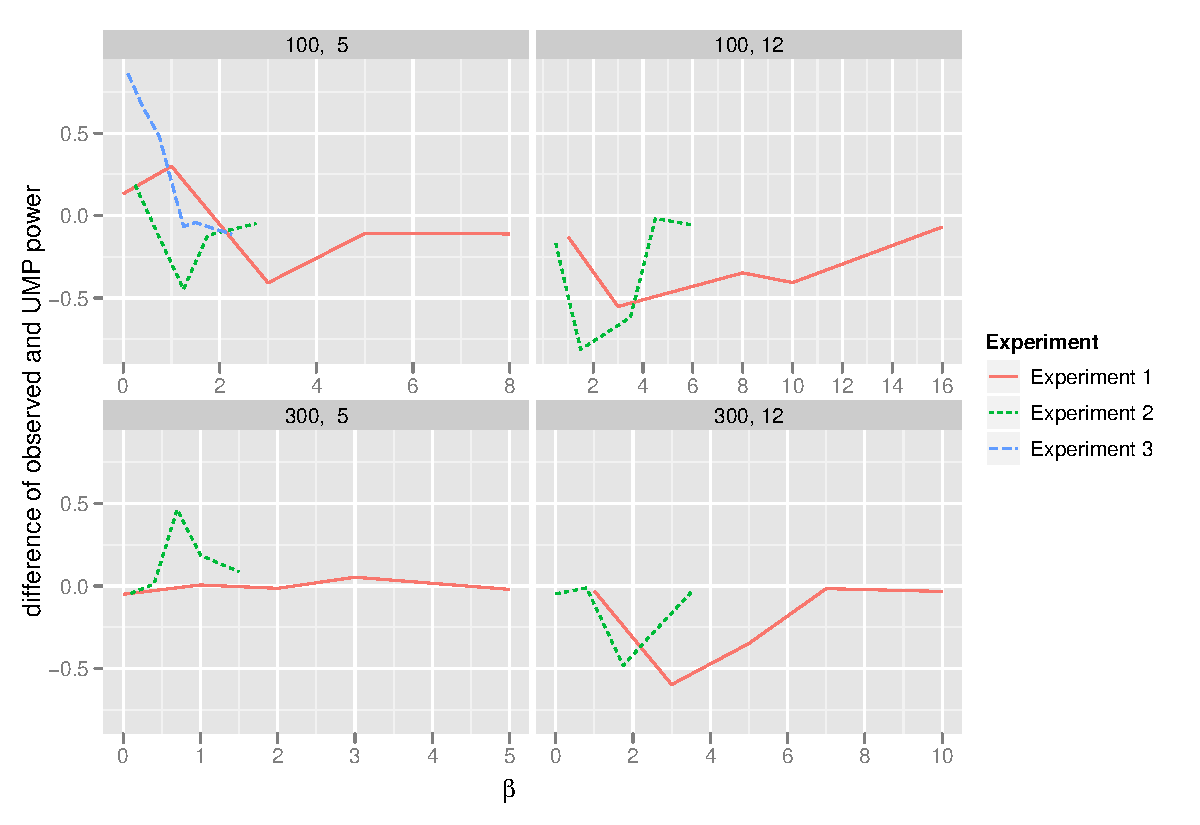
\includegraphics{power_diff_exp.pdf}}
%       \caption{Difference of Observed power from UMP test power obtained in three experiments for sample size $n= 100,300$ and $\sigma = 12,5$ and values of slope parameter $\beta$ as shown in Table \ref{tbl:experiment_params}.}
%       \label{fig:power_diff_exp}
%\end{figure*}


%\begin{figure*}[hbtp]
%   \centering
%       \scalebox{0.6}{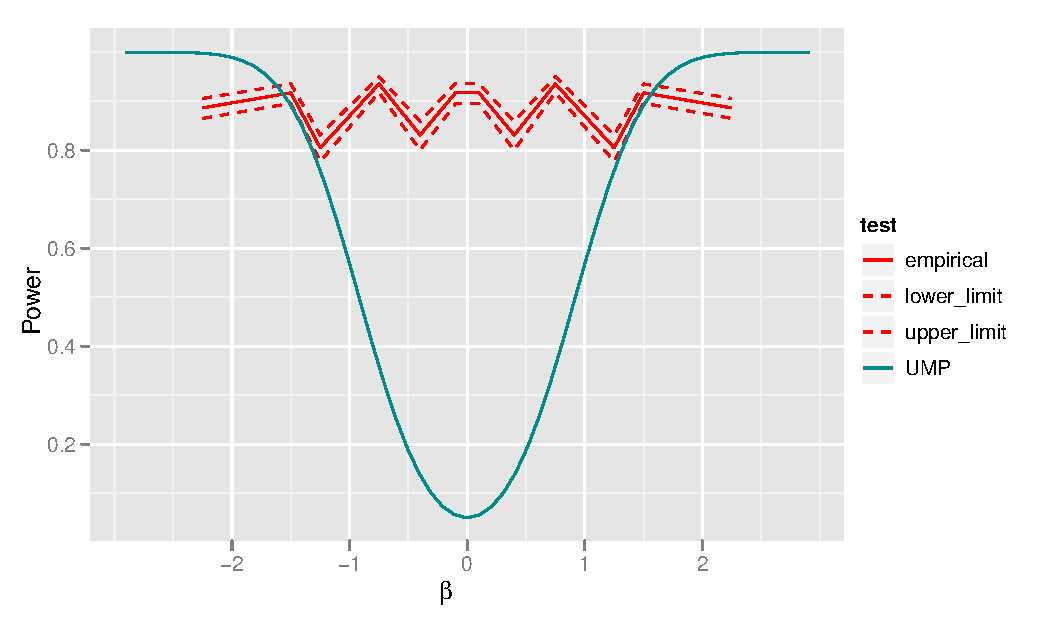
\includegraphics{power_observed_exp3.pdf}}
%       \caption{Observed power of visual test from equation \eqref{eqn:power_estimate} with pointwise 95\% confidence limits and the power of UMP test for sample size $n= 100$ and $\sigma = 5$ as per experiment 3. }
%       \label{fig:power_observed_exp3}
%\end{figure*}


\section{Results}

\subsection{Data Cleaning}

% In this process of collecting data some participants did not provide demographic information as we see in Table \ref{tbl:summary} that male and female participants do not add up to total participants. It is not clear why they did not provide the information. Now the concern arises whether we should keep their responses in the study. It is also possible that participants were not serious enough to provide feedback. 
%For each of the experiments we had a test plot (easy plot) for which they should have a correct evaluation without much effort.  This could be a criteria to determine their attentiveness in the study. For this we consider six different data cleaning criteria as shown below;

%{\bf Screening scenarios:}
Amazon Mechanical Turk workers are paid for their efforts, not substantial, but on the scale of the minimum wage of the USA. Some workers will try to maximize their earnings for minimum effort, which can affect the results from the data. For example, some workers may simply randomly pick a plot, without actively examining the plots in the lineup. For the purpose of identifying these participants and cleaning the data, we make use of one of the very easy lineups that every subject was exposed to.
For each subject we use a randomly selected easy lineup. If the subject failed to identify the actual data plot, we remove all of this subject's data from the analysis. If the answer on the lineup is correct, we remove this lineup from the analysis, but keep all of the remaining answers.
Table \ref{tbl:summary} tabulates the number of subjects, genders and lineups evaluated after applying the data screening procedure. 

%
%one of these was picked at random as the filtering lineup, and action was taken depending on whether they answered correctly or incorrectly. The data of participants who did not answer correctly was removed. 
%For the subjects, who correctly answered the filtering lineup, all of their data was kept, except for that particular lineup. That is, for each block of 10 lineups, only the data from 9 lineups was used for each subject.

%Amazon Mechanical Turk data suffers from the problem that some participants are trying to 'game' the system, because they are being paid for their efforts, not much by the standards of the US minimum wage, but enough to encourage honest efforts.  in our situation, these are participants who did not put in a best effort to identify the data plot, but just randomly picked a plot to maximize their 'winnings'.  In order to avoid using those results, we are comparing six different screening methods for excluded participants from the data analysis. 
%There are six suggested approach to clean the data. 
%They are
%\begin{enumerate}
%\item {\bf include all participants} and their evaluations
%\item exclude all participants' evaluations, who did {\bf not} share their {\bf demographic information} (age, gender education level -- all three pieces of information are either missing or all present).
%\item exclude participants' records, if {\bf none of the evaluations}  correctly identified the data plot -- every participant was shown a range of `easy' lineups.
%\item include participants' records, if   {\bf at least 20 percent} of the evaluations are {\bf correct}  -- based on ten evaluations per participants, two correct evaluations are significant evidence against a person just guessing
%\item include participants' records, if at least {\bf 50\% of all very easy lineups are correct} 
%\item use easy lineups as {\bf reference charts}: sample one easy lineup from a person's records. If that lineup is evaluated {\bf correctly}, include all (other) lineups of that person, otherwise exclude all lineup evaluations by this participant.
%\end{enumerate}

%\begin{table}[hbtp]
%\caption{Number of unique subjects and their total feedbacks after applying six screening process on all three experimental data sets. 
%Note that in some of the lines the number of male and female participants does not add up to the total number of participants. This is due to missing demographic information. \hh{Do we need this table or could we make this a visual comparison? For me, there's too many numbers with too many digits.}}
%\begin{center}
%\begin{tabular}{rrrrr|rrrr|rrrr}
%  \hline
%Screening &  \multicolumn{4}{c} {Experiment 1}  & \multicolumn{4}{c} {Experiment 2}  & \multicolumn{4}{c} {Experiment 3} \\
% \cline{2-5}  \cline{6-9}   \cline{10-13}
%criteria & Subj & Male & Fem & Total & Subj & Male & Fem & Total & Subj & Male & Fem & Total \\ 
%  \hline
%1 & 520 & 264 & 201 & 4914 & 390 & 203 & 182 & 4603 & 257 & 166 &  84 & 2830 \\ 
%  2 & 465 & 264 & 201 & 4624 & 385 & 203 & 182 & 4558 & 250 & 166 &  84 & 2782 \\ 
%  3 & 384 & 200 & 165 & 4187 & 384 & 199 & 181 & 4573 & 227 & 147 &  78 & 2648 \\ 
%  4 & 318 & 168 & 135 & 3395 & 378 & 195 & 179 & 4492 & 205 & 133 &  72 & 2393 \\ 
%  5 & 277 & 139 & 124 & 3008 & 374 & 193 & 177 & 4451 & 185 & 122 &  63 & 2121 \\ 
%  6 & 239 & 121 & 107 & 2317 & 351 & 185 & 164 & 3858 & 156 & 106 &  50 & 1681 \\ 
%   \hline
%\end{tabular}
%\end{center}
%\label{tbl:summary}
%\end{table}

\begin{table}[hbtp]
\caption{Number of subjects, gender and total lineups seen, and number of distinct lineups for all three experimental data sets. Note that in some of the lines the number of male and female participants does not add up to the total number of participants due to missing demographic information. }%\blue{Notice that we do not have data on one lineup (so we have only 29 lineups) for experiment 3 due to the screening process.}}
\begin{center}
\begin{tabular}{ccrrcc}
   \hline \hline
 Experiment & Subject & Male & Female & Responses &Lineup\\ 
    \hline
1 & 239 & 121 & 107 & 2249 &  60 \\ 
  2 & 351 & 185 & 164 & 3636 &  70 \\ 
  3 & 155 & 103 &  52 & 1511 &  29 \\  
   \hline
\end{tabular}
\end{center}
\label{tbl:summary}
\end{table}


\subsection{Model fitting}
\noindent For each parameter combination, the effect is computed as 

\[
E=\sqrt {n} \cdot \beta/\sigma.
\]

The model in Equation \ref{eqn:mixed} is fit using $E$ as the only fixed effect covariate without intercept., i.e. 
 $W_{\ell i} = E_{\ell i}$ in Equation \ref{eqn:mixed}. 
Instead of fitting an intercept, we make use of a fixed  offset of $\log(0.05/0.95)$ so that the estimated power has a fixed lower limit at 0.05 (Type-I error) when $E=0$. Different subjects are expected to have different skill levels in evaluating lineups. We account for this by using subject-specific random  slopes for  effect ($E$). 

For experiment 3 we so fit intercepts: both a fixed effect and subject-specific random intercepts, since forcing power
%While for experiment 1 and 2 we don't allow intercept but offset, for experiment 3 an intercept is estimated to allow the power curves to go above 0.05 when $E=0$. This is because forcing power 
to be fixed at 0.05 for $E=0$ is not justified by the data from experiment 3.% (Figure \ref{fig:power_loess_effect}). *** You cannot reference the figure before you explain it!!!

%For all the three experiments, each subject saw a lineup just once. This does not allow fitting a lineup random effect, in addition to a subject random effect, but it does simplify the model since $\tau_{\ell i} = \tau_i$. 

The subject-specific probability, $p_i$, of successful evaluation of a lineup is then estimated using Equation \ref{eqn:mixed_power}. For computation we use R \citep{R} package lme4 \citep{lme4:2011}.

Table \ref{tbl:model_par} shows the parameter estimates of the mixed effects model of the subject-specific variation. \green{The fixed effects estimates indicate that for all experiments as the effect increases the proportion correct increases. For experiment 3 it is very weak. The subject-specific variability is smaller for experiment 1, and relatively large for experiment 3.} %The larger variability in the response data for experiment 3% as we see in Figure \ref{fig:power_loess_effect}  *** You cannot reference the figure before you explain it!!!
%contributes to the random effect variance estimate be much larger compared to those of other experiments. For the same reason we see the standard error for intercept estimate is much higher as well. Also notice the slope estimate for experiment three is lowest as well. It is because for small parameter values the power is much higher for experiment 3.  % \green{What do we learn about the models from these parameter estimates? Explain this here too.}

%\green{This section needs to have sufficient detail of the model fitting, output and diagnostics to feed into the next few sections discussing the findings.}

\begin{table}[hbtp]
\caption{Parameter estimates of model in Equation \ref{eqn:mixed}. Estimates are highly significant with $p$-value $<$  0.0001 for all three experiment data.}
\begin{center}
\begin{tabular}{cr@{.}lcc}
  \hline \hline
 &  \multicolumn{3}{c} {Fixed effect}  & Random effect\\
 \cline{2-4}
 Experiment & \multicolumn{2}{l}{Estimate}  &Std. error & Variance\\
  \hline
  1 & 0&39 & 0.0094 & 0.0080 \\ 
  2 & 1&21 &  0.0197 &  0.0443 \\ 
  3 & 0&59 (Intercept)  &   0.1668 & 1.9917\\ 
     & 0&21 (Slope)    &  0.0511     &  0.0245\\ 
     &-0&78 (correlation) & & \\
   \hline
\end{tabular}
\end{center}
\label{tbl:model_par}
\end{table}

\subsection{Power comparison}

\noindent Figure \ref{fig:power_loess_effect} shows the power against effect for the three experiments. Data values are represented as dots with size indicating count at this value. The loess curves fit the data, estimating the observed power for different effect sizes, with grey bands indicating simultaneous bootstrap confidence bands. For comparison, the dashed lines show the corresponding power curves of the conventional tests. The observed power for experiments 1 and 2 are lower than the power of the conventional test. This is not a surprise -- it is not expected that visual inference will beat conventional tests, in the scenario when assumptions are satisfied. It is encouraging to see that visual inference mirrors the power vs effect relationship of conventional testing, and comes quite close in experiment 2, where scatterplots are used as the test statistic. 

\begin{figure}[hbtp]
   \centering
       \scalebox{0.55}{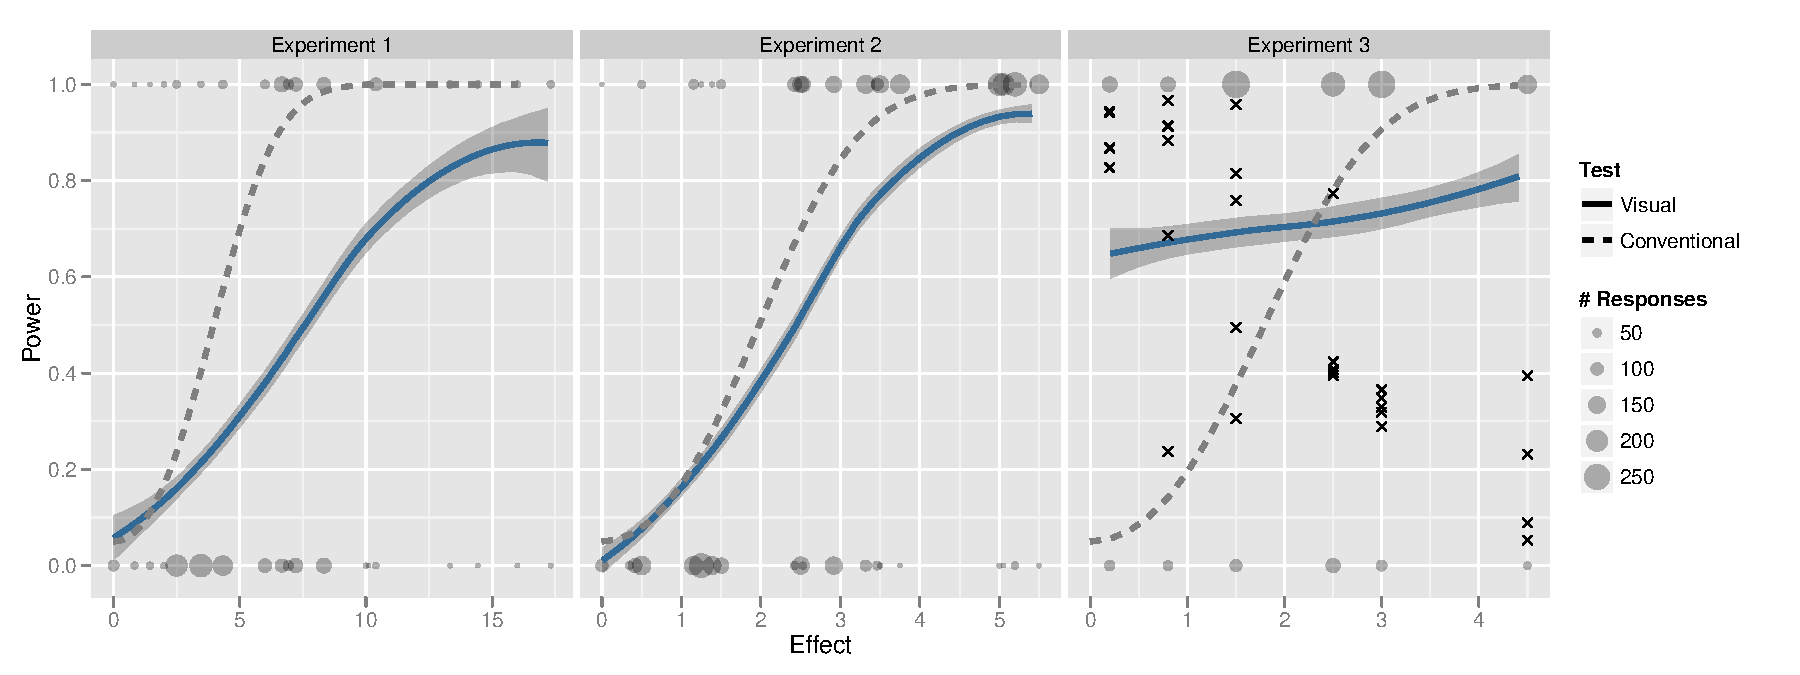
\includegraphics{power_loess_effect.pdf}}
       \caption{Power in comparison to effect for the three experiments. Points indicate subject responses, with size indicating count. Responses are 1 and 0 depending on the success or failure respectively to identify the actual plot in the lineup. \blue{The loess curve (blue) estimates the observed power}, and grey bands show simultaneous bootstrap confidence band.  Conventional test power is drawn as a dashed line. For experiment 3, conventional power is based on the slopes of the linear part of the non-contaminated data. Power for contaminated data is shown by cross mark.}
       \label{fig:power_loess_effect}
\end{figure}

Results for experiment 3, are quite different. This is the situation where we expect to see the potential of visual inference, and indeed we do: the power of visual inference is always high, and much higher than the conventional test at small effect sizes. There is no actual conventional power in this situation, because assumptions are violated. It is computed assuming that there is no contamination, using the non-contaminated part of the simulation model. The  conventional power of true effect of the contaminated data is computed anyway and presented in figure \ref{fig:power_loess_effect} by cross marks. For this we obtain the estimated slope for the contaminated data and compute the estimated effect for which conventional power is calculated. Notice that the power structure is completely broken for contaminated data. For smaller original effect we get huge power and that explains why we see so many small $p$-values for experiment 3

It is really curious to see in the results of experiment 3 that the power of the visual test is really high when effect is small. These results are based on whether the subject correctly picked the actual data plot, regardless of reason. Although they were asked to select the plot that exhibited the highest association between the two variables, it may have been that they were cueing to the cluster of contaminated data. This will be explored further in Section \ref{sec:TypeIII}. 

%(scatter plot) is better than what we observed for experiment 1 (box plot). For experiment 3, observed power is always above the conventional test power since for contaminated data we can visually see a trend while conventional test fail to address that.

It can also be seen that at effect $E=0$, the power is close to 0.05 (Type-I error) for both experiments 1 and 2. For experiment 3 the scenario is different. The contamination in the data is visible which sets the lower limit of proportion correct at a higher value.  

%The power curves obtained by fitting model \ref{eqn:mixed} to the data for all the experiments applying different screening criteria is shown in figure \ref{fig:power_screening}. This shows how the screening criteria may affect the results. The corresponding power curves of conventional test are also shown. Notice that no mater what criteria we apply the result does not change much for experiment 2. Also, estimated power curve with criteria 5 for experiment 3 is above the conventional test power curve.


%
%\begin{figure}[hbtp]
%   \centering
%       \scalebox{0.70}{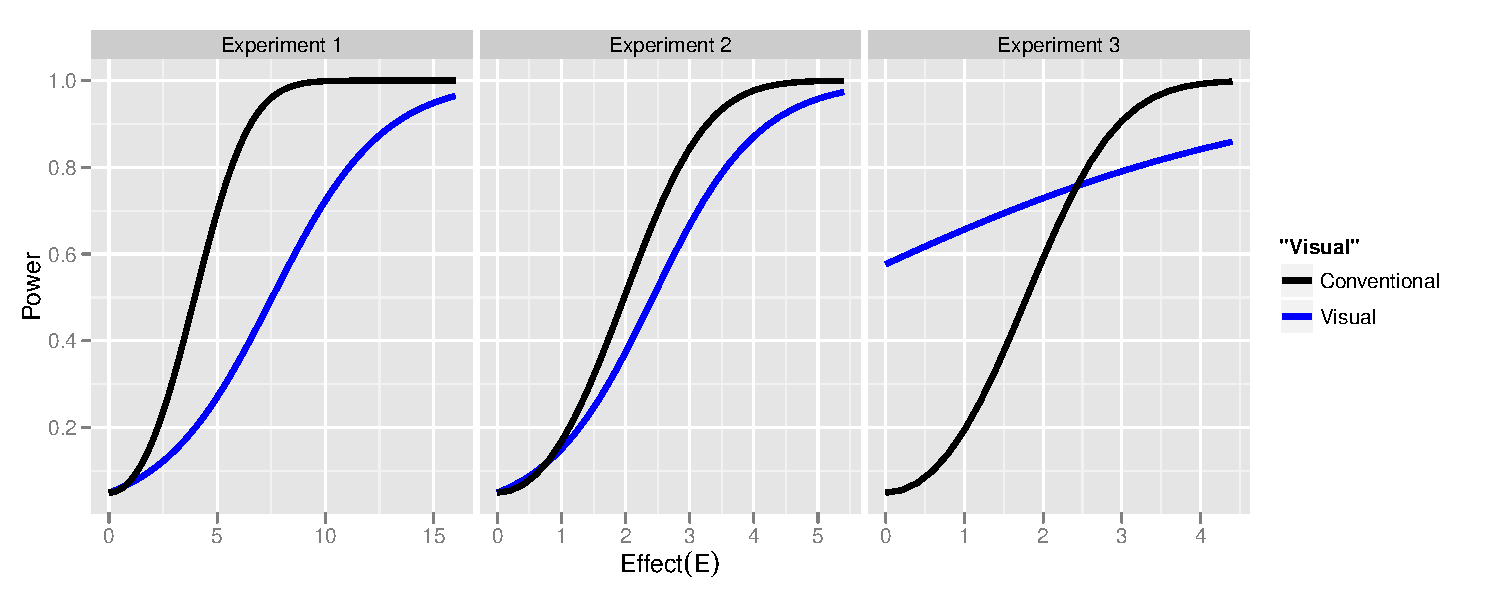
\includegraphics{power_mixed.pdf}}
%       \caption{The overall power estimated from model \ref{eqn:mixed} are shown. The corresponding power curve for conventional test is shown for comparison.}
%       \label{fig:power_mixed}
%\end{figure}



%Each participant was shown a sequence of 10 lineup plots.  In total, 3629 lineups were evaluated by 324 people coming from many different locations across the globe.  The results of the experiment are summarized in Figure \ref{fig:power_observed} which shows the observed power from the survey data calculated using equation \eqref{eqn:power_estimate} along with 95\% confidence interval calculated using Fisher's exact method.

%\begin{figure*}[hbtp]
%   \centering
%       \scalebox{0.45}{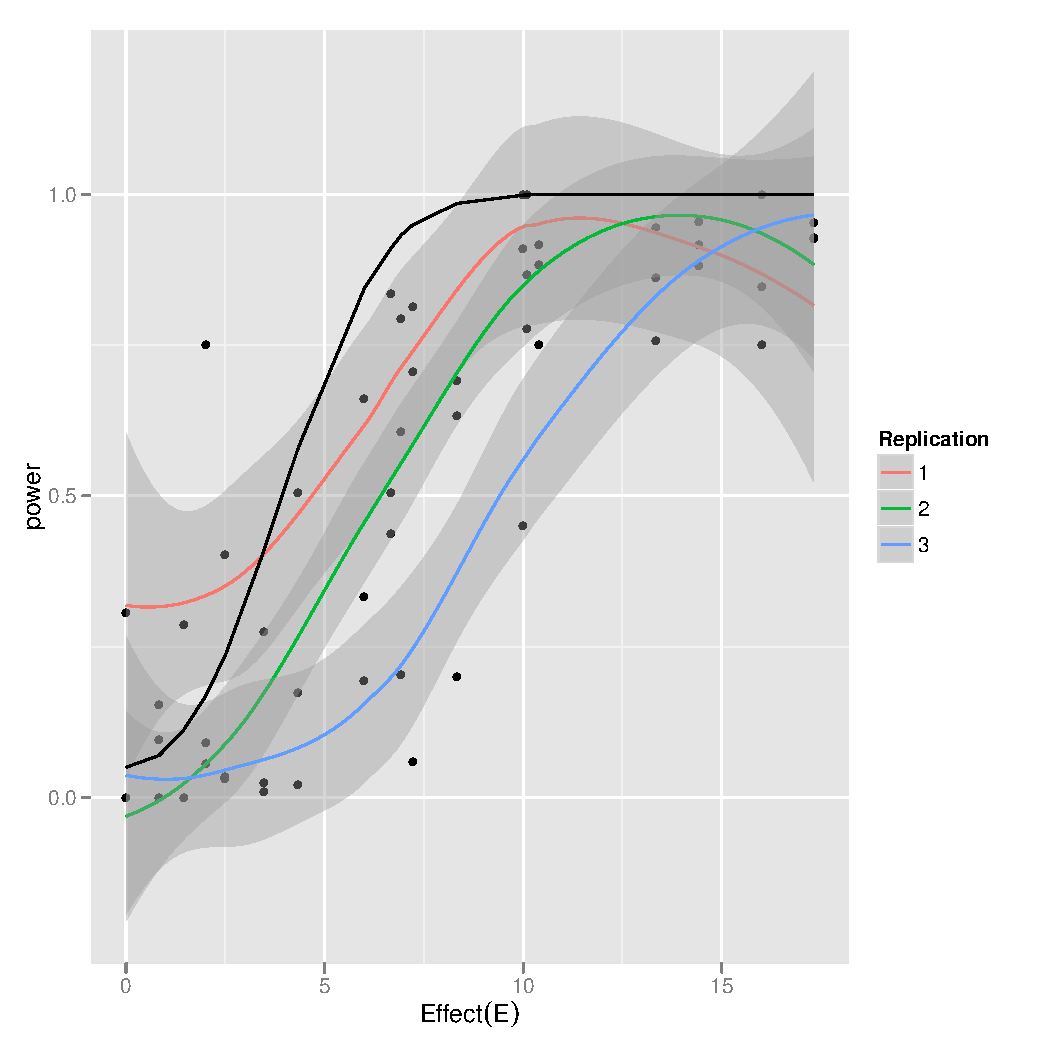
\includegraphics{effect_power_exp1.pdf}}
%       \scalebox{0.45}{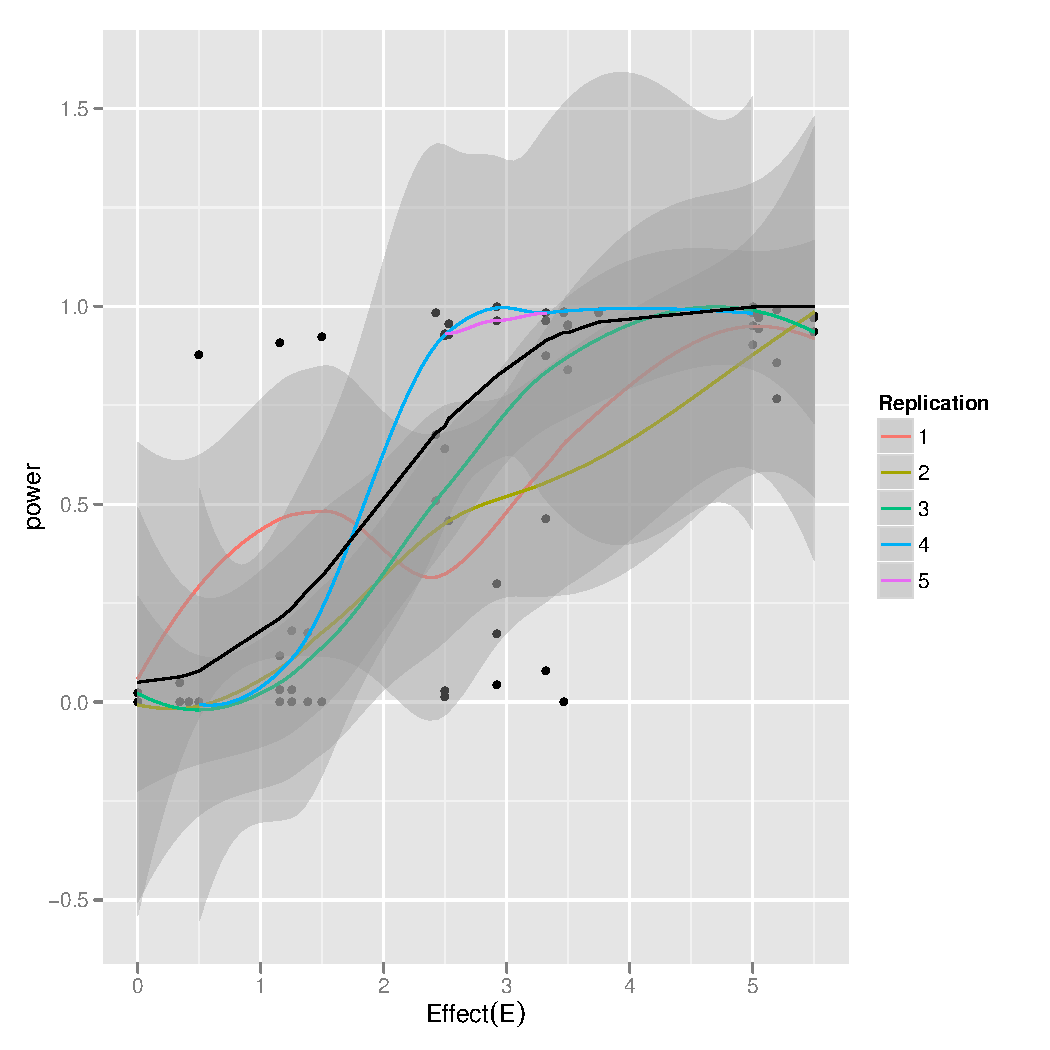
\includegraphics{effect_power_exp2.pdf}}
%       \caption{Observed power shown by loess smoother and the power of conventional test for different effect size $E$ as per experiment 1 and 2.}
%       \label{fig:power_effect1}
%\end{figure*}

%\begin{figure*}[hbtp]
%   \centering
%       \scalebox{0.45}{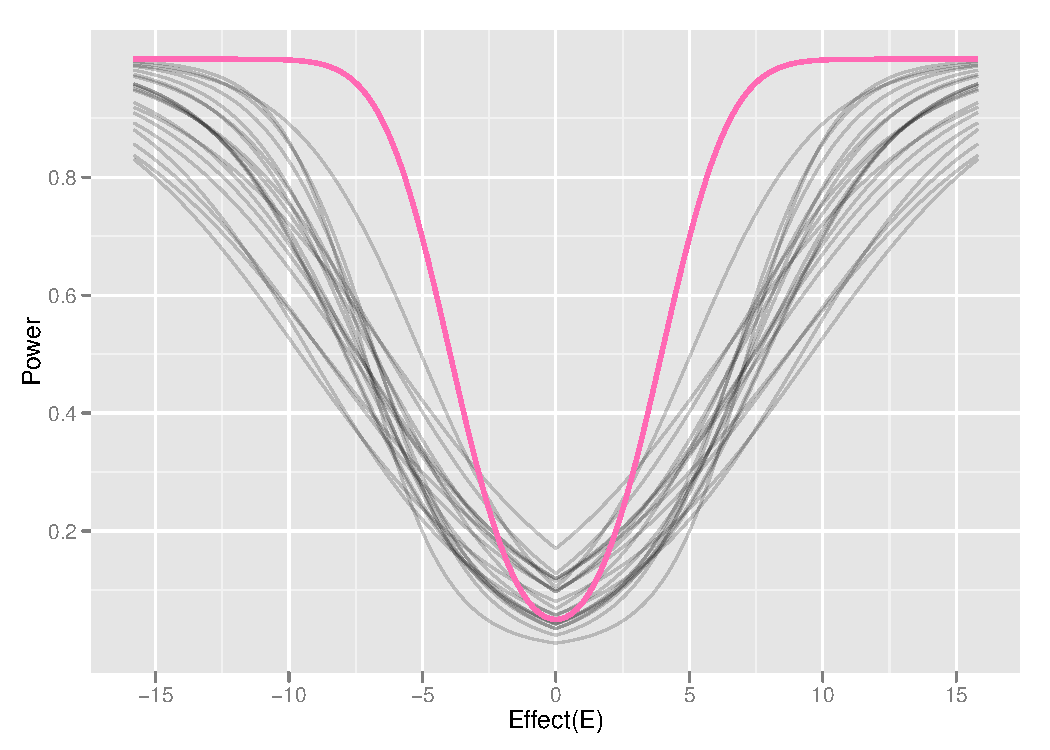
\includegraphics{effect_power_subject_exp1.pdf}}
%       \scalebox{0.45}{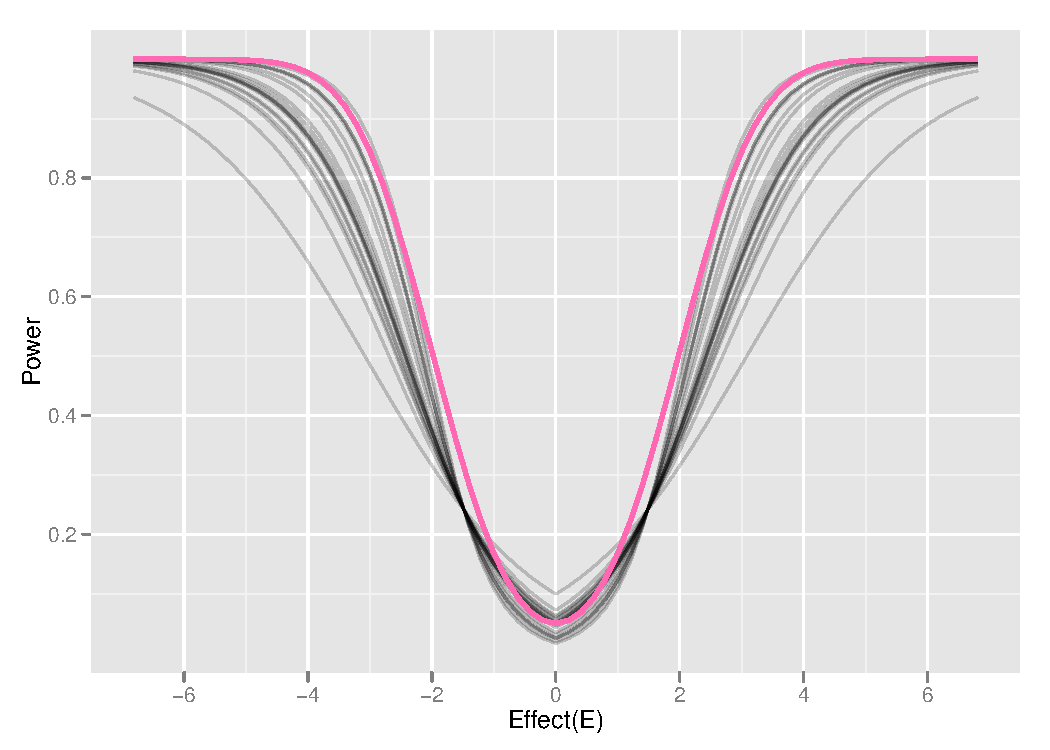
\includegraphics{effect_power_subject_exp2.pdf}}
%       \caption{Subject specific power obtained from equation \eqref{eqn:effect} and the power of UMP test for different effect size $E$ as per experiment 1 and 2.}
%       \label{fig:power_effect_subject1}
%\end{figure*}


%\begin{figure*}[hbtp]
%   \centering
%       \scalebox{0.4}{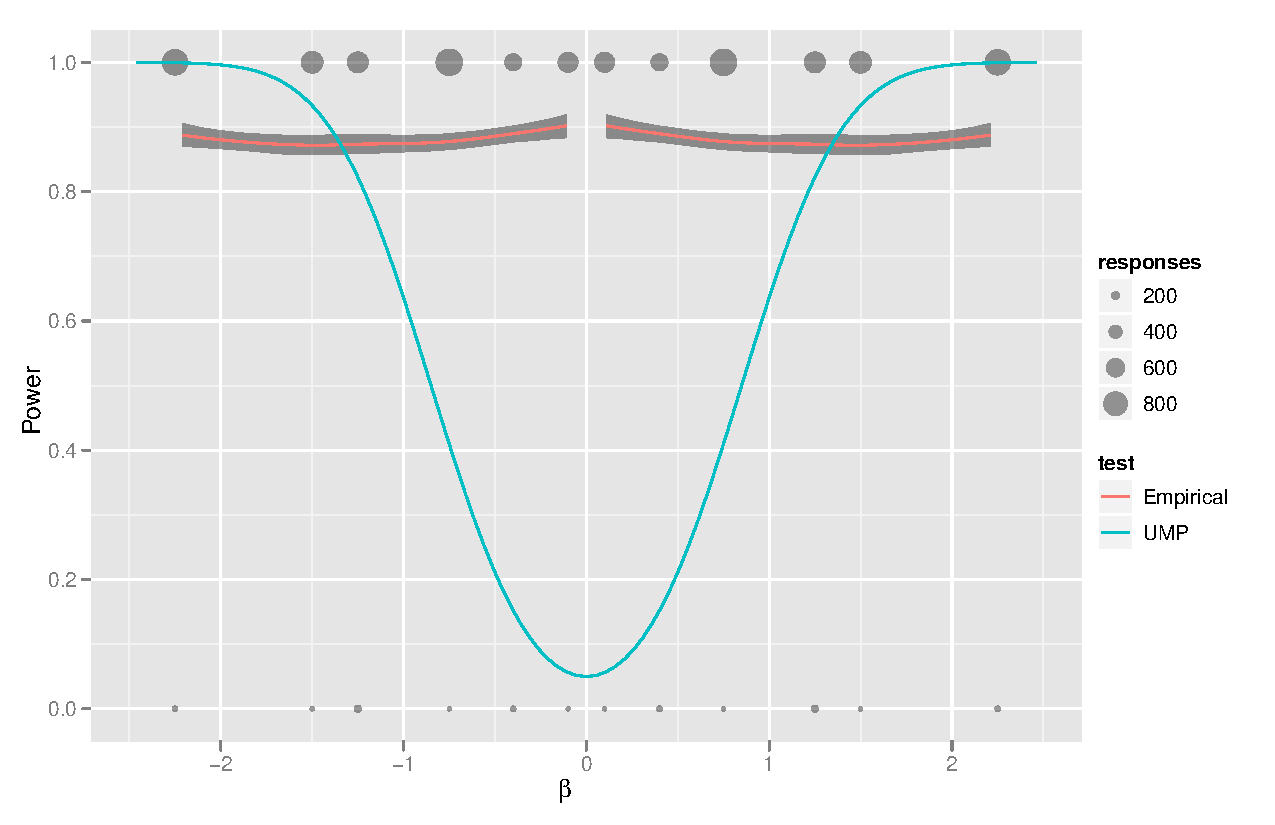
\includegraphics{power_loess_exp3.pdf}}
%       \caption{Observed power shown by loess smoother with simultaneous bootstrap confidence band and the power of conventional test for sample size $n= 100$ and $\sigma = 5$ as per experiment 3. Notice that for experiment 3, power does not seem to depend on the parameter $\beta$. \blue{Di/Heike, I am not sure how I can relate this to demonstrate the power of visual inference when normal conditions are not met. Does this really test our hypothesis $H_0: \beta=0$ or some other hypothesis about the existence of cluster in the data?}}
%       \label{fig:power_loess3}
%\end{figure*}

%\begin{figure}[hbtp]
%   \centering
%       \scalebox{0.40}{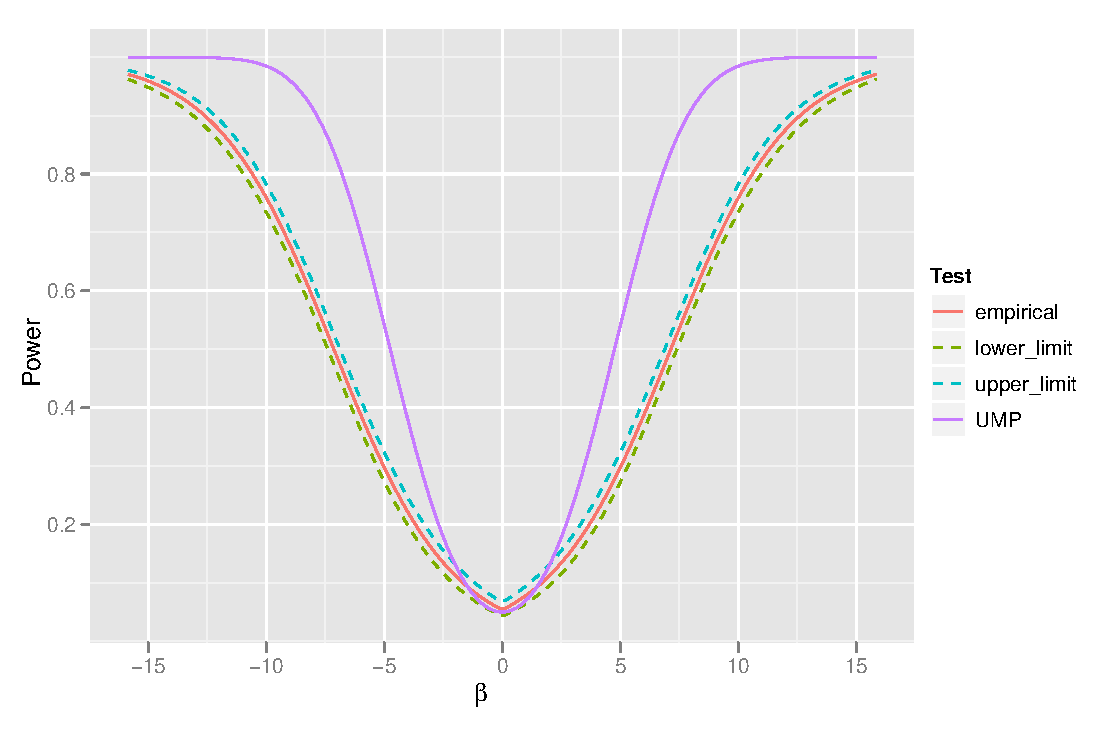
\includegraphics{power_model.pdf}}
%       \caption{Estimated power curve from equation \eqref{eqn:power} along with 95\% confidence interval for sample size $n$ = 100 and $\sigma$ = 12.  The corresponding power curve for Uniformly Most powerful (UMP) test is shown for comparison.}
%       \label{fig:power_model}
%\end{figure}

%We fit model \eqref{eqn:mixed} to the survey data obtained from the simulation experiment. The estimated overall power curve obtained from equation \eqref{eqn:power} is shown in Figure \ref{fig:power_model}. Model \ref{eqn:mixed} also gives the subject specific power curves shown in Figure \ref{fig:power_subject}. The plot includes 20 randomly selected subject-specific power curves. Notice that the power curve estimated for one subject is above the UMP test power curve. 

%\begin{figure}[hbtp]
%   \centering
%       \scalebox{0.45}{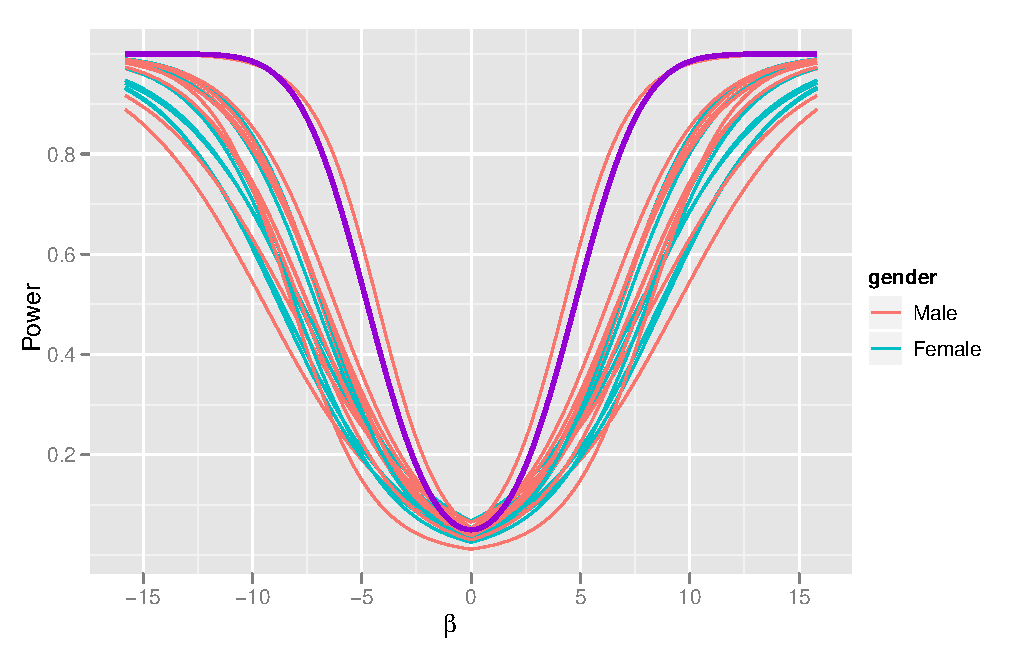
\includegraphics{power_subject.pdf}}
%       \caption{Estimated subject specific power curve from model \ref{eqn:mixed} for sample size $n$ = 100 and $\sigma$ = 12.  The corresponding power curve for Uniformly Most powerful (UMP) test is shown for comparison.}
%       \label{fig:power_subject}
%\end{figure}

\subsection{Subject-specific variation}

%Different subjects are expected to have different skill levels in evaluating lineups. This is accounted for in the mixed effects model (Equation \ref{eqn:mixed}).   
 The estimated subject-specific power curves are shown in \blue{Figure \ref{fig:power_mixed_subject} (light grey lines). The blue curve is the overall} average power estimated from the model, and for comparison, the grey dashed lines are the power curves for the conventional test. Subject-specific power is quite different for three experiments. In experiment 1 subjects performed similarly, and substantially worse than the conventional test. In experiment 2 there is more variability between subjects, with some doing better than the conventional test on small effects. In experiment 3 there is the most subject-specific variation. Some subjects performed substantially better than the conventional test, and on average the visual test was better. 

\begin{figure}[hbtp]
   \centering
       \scalebox{0.60}{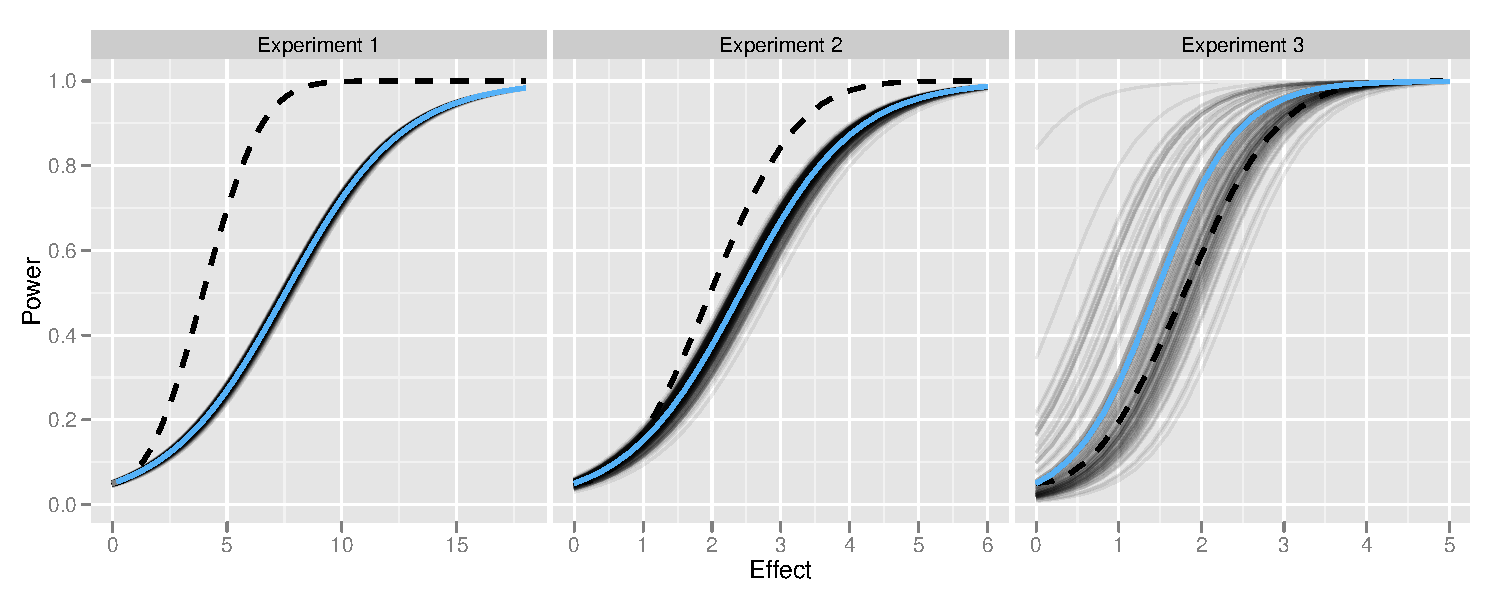
\includegraphics{power_mixed_subject.pdf}}
       \caption{Subject-specific  power estimated from model \ref{eqn:mixed} are shown. The corresponding power curve for conventional test (dashed line) is shown for comparison. The overall average power curve estimated from the model is shown (light blue).}
       \label{fig:power_mixed_subject}
\end{figure}


\subsection{Estimating the $p$-value in the real world} 

%\green{third experiment doesn't really have a p-value, does it? Need to explain this. Why are there still so many small p-values in experiment 3?} \blue{$p$-values are computed fitting the full model to the contaminated data anyway. So many small p-values are coming from the fact that contamination makes the slope negatively significant. For example, for some slope the contamination reverses the slope (positive to negative) and negative slope got significant. It is like the effect of influential outlier.}

In the real setting, where visual inference is to be useful, there will be no conventional tests $p$-values. Assessing the strength of perceived structure is a critical component of visual inference. In experiments 1 and 2, there is a $p$-value associated with the actual data plot in each lineup. As the $p$-value increases the proportion of correct responses falls (Figure \ref{fig:pval_pcorrect}), which is evidence of direct association between proportion of correct responses and conventional test $p$-values. When $p$-value is larger than 0.15, it is very uncommon for subjects to correctly identify the actual data plot in the lineup.

\begin{figure*}[hbtp]
   \centering
       \scalebox{0.6}{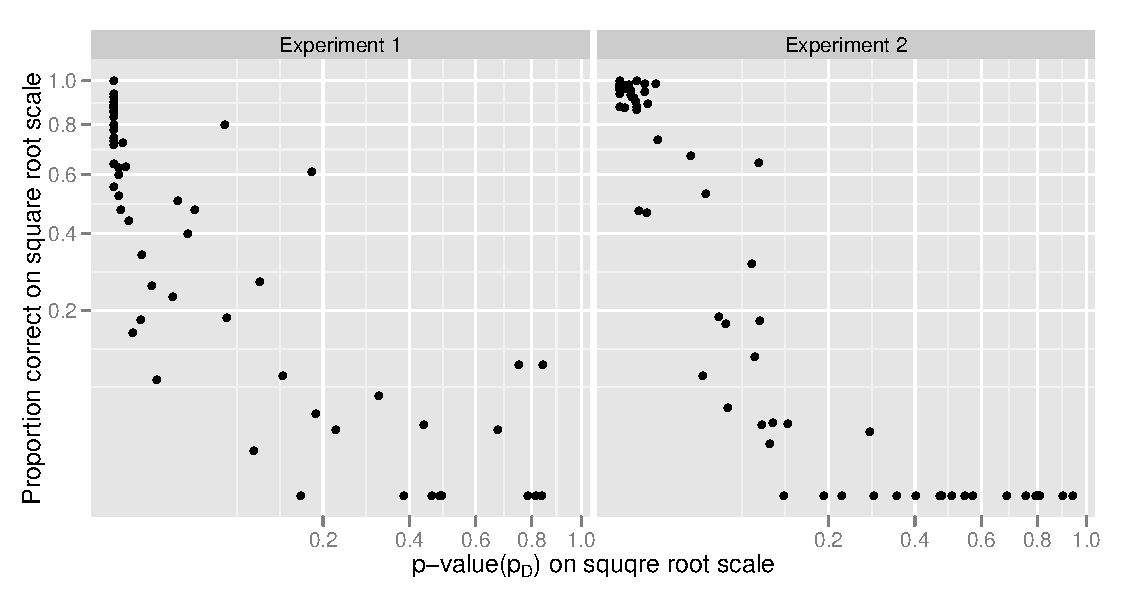
\includegraphics{p_val_prop_correct.pdf}}
       \caption{Proportion of correct responses decreases rapidly with the increase of p-value. After p-value exceeds 0.15 it is very unlikely to identify the actual plot. The theoretical justification of this is shown in Figure \ref{fig:pval_power}. }
       \label{fig:pval_pcorrect}
\end{figure*}

From the experimental data the visual $p$-values are computed using Definition \ref{dfn:pvalue}. Figure \ref{fig:pval_definition} displays this visual $p$-value for each lineup against the conventional $p$-value.  The pattern of visual $p$-value is interesting. If there is a signal in the data plot, visual $p$-value has a tendency to take a smaller value (small enough to reject $H_0$) and if not it takes a larger value (large enough to not reject $H_0$) giving a clear indication to reject $H_0$ or not. This is why we do not see lot of visual $p$-values in between 0.05 and 0.8 especially for experiment 2. This guide the researcher to make decision confidently while conventional $p$-values take some marginal $p$-values for which researchers get confused whether to reject or 'not reject' $H_0$. For visual test this is not common.  

\begin{figure*}[hbtp]
   \centering
       \scalebox{0.6}{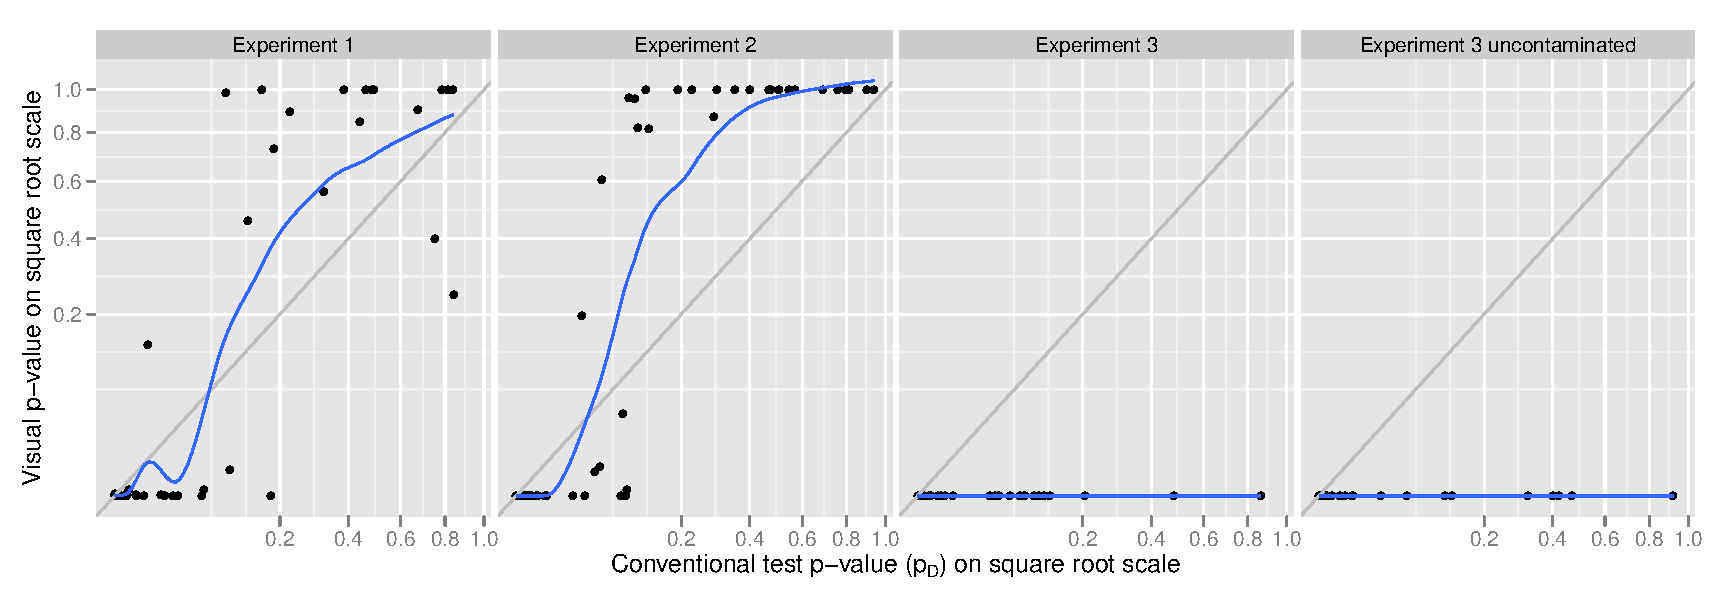
\includegraphics{p_val_definition.pdf}}
       \caption{Conventional test $p$-value ($p_D$) vs visual $p$-value obtained from the definition . Values are shown on square root scale. }
    %   \hh{Mahbub, another change: could you change the y label to 'estimate of visual p-value $\hat{p_D}$ ?}
       \label{fig:pval_definition}
\end{figure*}

We also see the same pattern from the loess smoother fitted through the points in Figure \ref{fig:pval_definition}. The sigmoid shaped loess curves indicate a clear separation of visual $p$-values. For experiment 1, most of the visual $p$-values are above 0.4 when conventional $p$-values are above 0.2. This is more evident for experiment 2 where most of the visual $p$-values are above 0.8. For experiment 3, we see all the visual $p$ values are almost zero no matter what the conventional $p$-values are. This is expected since conventional test fails to reject $H_0$ where we should reject and visual test does the job nicely.

%With multiple subjects it is possible to estimate the visual $p$-value, and a measure of plot signal strength. The visual $p$-value is calculated from the binomial formula (Equation \ref{binom}). Assuming $H_o$ is true, the probability of picking the actual data plot by chance is $1/m$, and the visual $p$-value is the probability that $x$ or more subjects select that plot. Figure \ref{fig:pval_definition} displays this visual $p$-value for each lineup against the conventional $p$value. 




%Similary, the strength of the signal, is calculated using the proportion of subjects picking actual data plot. It is closely related to the power of the test. From Equation \ref{eqn:power_estimate}  we can write $1 - E[N_m]/K \approx (m-1)E[p_D] $. This gives the signal strength estimate as  
%\[
%\hat p_D= (1- {u}/{K})/({m-1})
%\]
%where $K$ is the total number of independent evaluations on a lineup and $u$ is the number of successful evaluations. Figure \ref{fig:pval_plot_signal} shows the plot signal strengths in relation with conventional test $p$-values, on a square root scale. For experiment 3, technically, there are no conventional $p$-values, but the $p$-values are computed in the same manner as experiment 2, assuming that the data satifies the assumptions. The blue line is a loess fit to the data, and the grey line indicates equality of the two axes. The relationship between the conventional $p$-value and the plot signal strength is very strong, particularly when the values are small. As the conventional $p$-value increases, the estimated signal strength increases -- subjects find it harder to detect the actual data plot at larger $p$-values. The rise is very sharp for experiment 1, which indicates that subjects have a harder time detecting the actual data plot for even small $p$-values. 

%\green{Where is Figure \ref{fig:pval_definition} referred to and discussed?}
% \blue{Are we going to keep both figures \ref{fig:pval_definition} and \ref{fig:pval_plot_signal}?}
%
%\green{Explain why the term ``plot signal'' is introduced}

%, to assess the signal strength we examine the proportion of correct picks, with multiple users and the $p$-value of the actual data plot. For experiment 3 the \green{How is p-value calculated here?} Figure \ref{fig:pval_pcorrect} \blue{(should I bring this figure back?)}  displays scatterplots of these two variables for each experiment. As the $p$-value increases the proportion of correct responses falls, evidence of direct association between proportion of correct responses and conventional test $p$-values. When $p$-value is larger than 0.15, it is almost impossible to correctly identify the observed plot in the lineup. We observed this for both experiment 1 and 2. For experiment 3, the scenario is different, because there are two structures, the association between variables, and the cluster of contaminated points.% as in this case people might have observed something other than the effect $E$.

%Yet, it is possible to obtain an estimate the strength of the signal in the actual data plot, when there are multiple evaluations, using Lemma \ref{lemma}. 


%Note that $\hat{p}_D$ is bounded within $(0, 1/(m-1))$. This estimate has to be interpreted carefully, since the choice of a large lineup size, $m$, will make the value look `significant' in a conventional sense. Values close to the upper bound of $1/(m-1)$ should therefore be interpreted as `at least as high', rather than their actual numeric value.
%\hh{For $p$-values below $1/(m-1)$ visual $p$-values are very similar to actual $p$-values, the correlation for those values is: 0.36, 0.79, and -0.48 based on $n_1 = 44, n_2 = 45$, and $n_3= 26$ lineups, respectively.  }  \blue{This is not happening as we see in figure \ref{fig:pval_plot_signal}. But it is true for experiment 2, right?. }
%is equivalent to conventional test $p$-value when $p$-value is less than or equal to $1/(m-1)$.  
%and beyond that the plot signal strength levels off on a point bigger than 0.05. Thus if plot signal strength is less than 0.05, we may decide to reject the null hypothesis.





%\begin{figure*}[hbtp]
%   \centering
%       \scalebox{0.5}{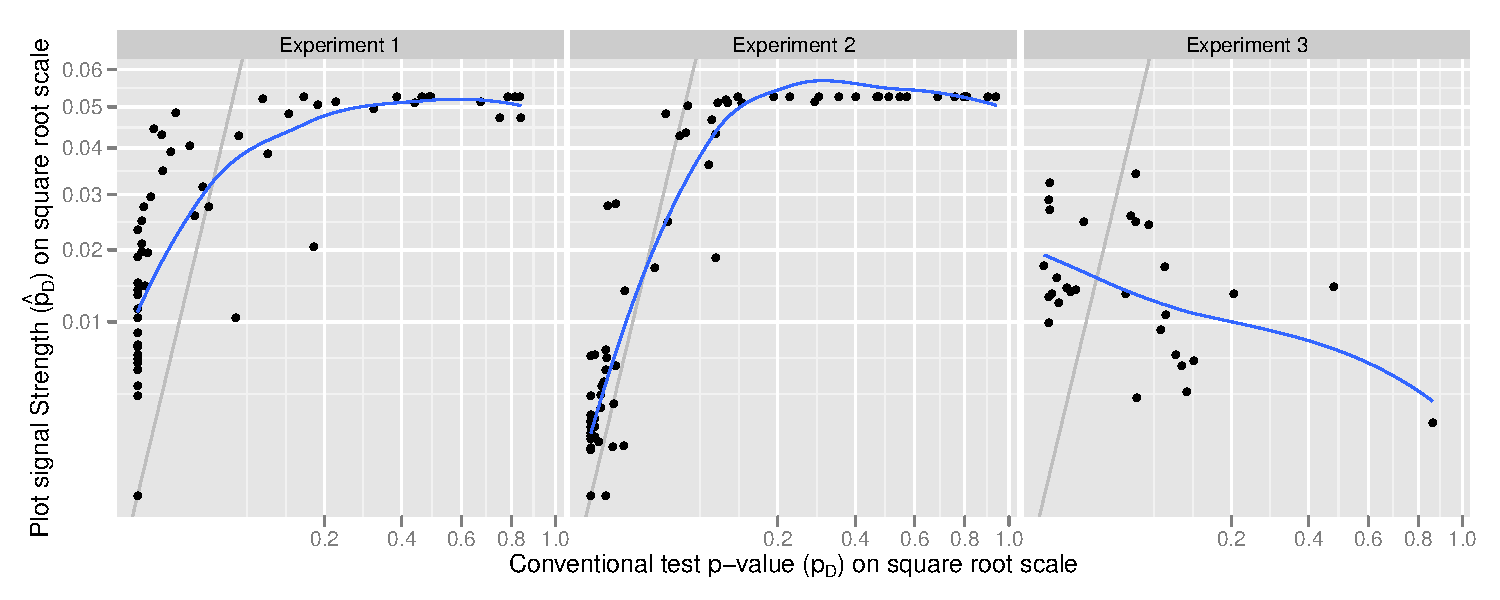
\includegraphics{p_val_plot_signal.pdf}}
%       \caption{Conventional test $p$-value ($p_D$) vs plot signal strength ($\hat p_D$). The solid line is a 45 degree line which represents the equity shown in Equation \ref{eqn:power_estimate}. p-values are shown on square root scale scale.}
%    %   \hh{Mahbub, another change: could you change the y label to 'estimate of visual p-value $\hat{p_D}$ ?}
%       \label{fig:pval_plot_signal}
%\end{figure*}

\subsection{Do people tend to pick the lowest $p$-value?}

One assumption made in order to calculate the effect of lineup size in the calculations of visual $p$-value and signal strength was that subjects would tend to pick the plot in the lineup that had the strongest signal. In experiments 1 and 2, this corresponds to the plot with the smallest $p$-value. This can be examined for the data collected, to see if this assumption is, indeed, reasonable. %In Section \ref{sec:size} in order to make comparisons with conventional tests an assumption was made that the subject would pick the plot in the lineup that had the lowest $p$-value. In this section we take a look at the picks that subjects made, to see if this is, indeed, true. 

Figures \ref{fig:P-val_log} and \ref{fig:P-val_log2} show the selection counts and $p$-values of all plots for each lineup in experiments 1 and 2, respectively. In each of these plots, the log of $p$-value for each plot in the lineup is plotted horizontally and the count of the number of subjects who selected this plot is displayed vertically. The dot represents this point, and the lines connect vertically with 0 count. Each row corresponds to a different $\beta$ value ordered top to bottom from lowest to highest. Columns correspond to the other levels of the experiment, sample size $(n)$, error standard deviation $(\sigma)$ and replicate. (Empty cells indicate no lineup shown with this combination.) Red indicates the plot with the lowest $p$-value in the lineup. (Blue indicates the plot of the actual data when it is different from that with the lowest $p$-value.) In both experiments as $\beta$ gets larger (stronger effect) people tended to select the plot with the lowest $p$-value. This is less so the case when $\beta$ is small, when standard deviation is large and sample size is small. The results are clearer for experiment 2, that used a continuous covariate. But even when they didn't pick the plot with the lowest $p$-value they tended to oscillate their choices between the several low $p$-value plots. So for most subjects, the assumption that they pick the plot with the smallest $p$-value would appear to be reasonable, and the actual power of the visual test should be close to the expected power.

\begin{figure*}[hbtp]
   \centering
       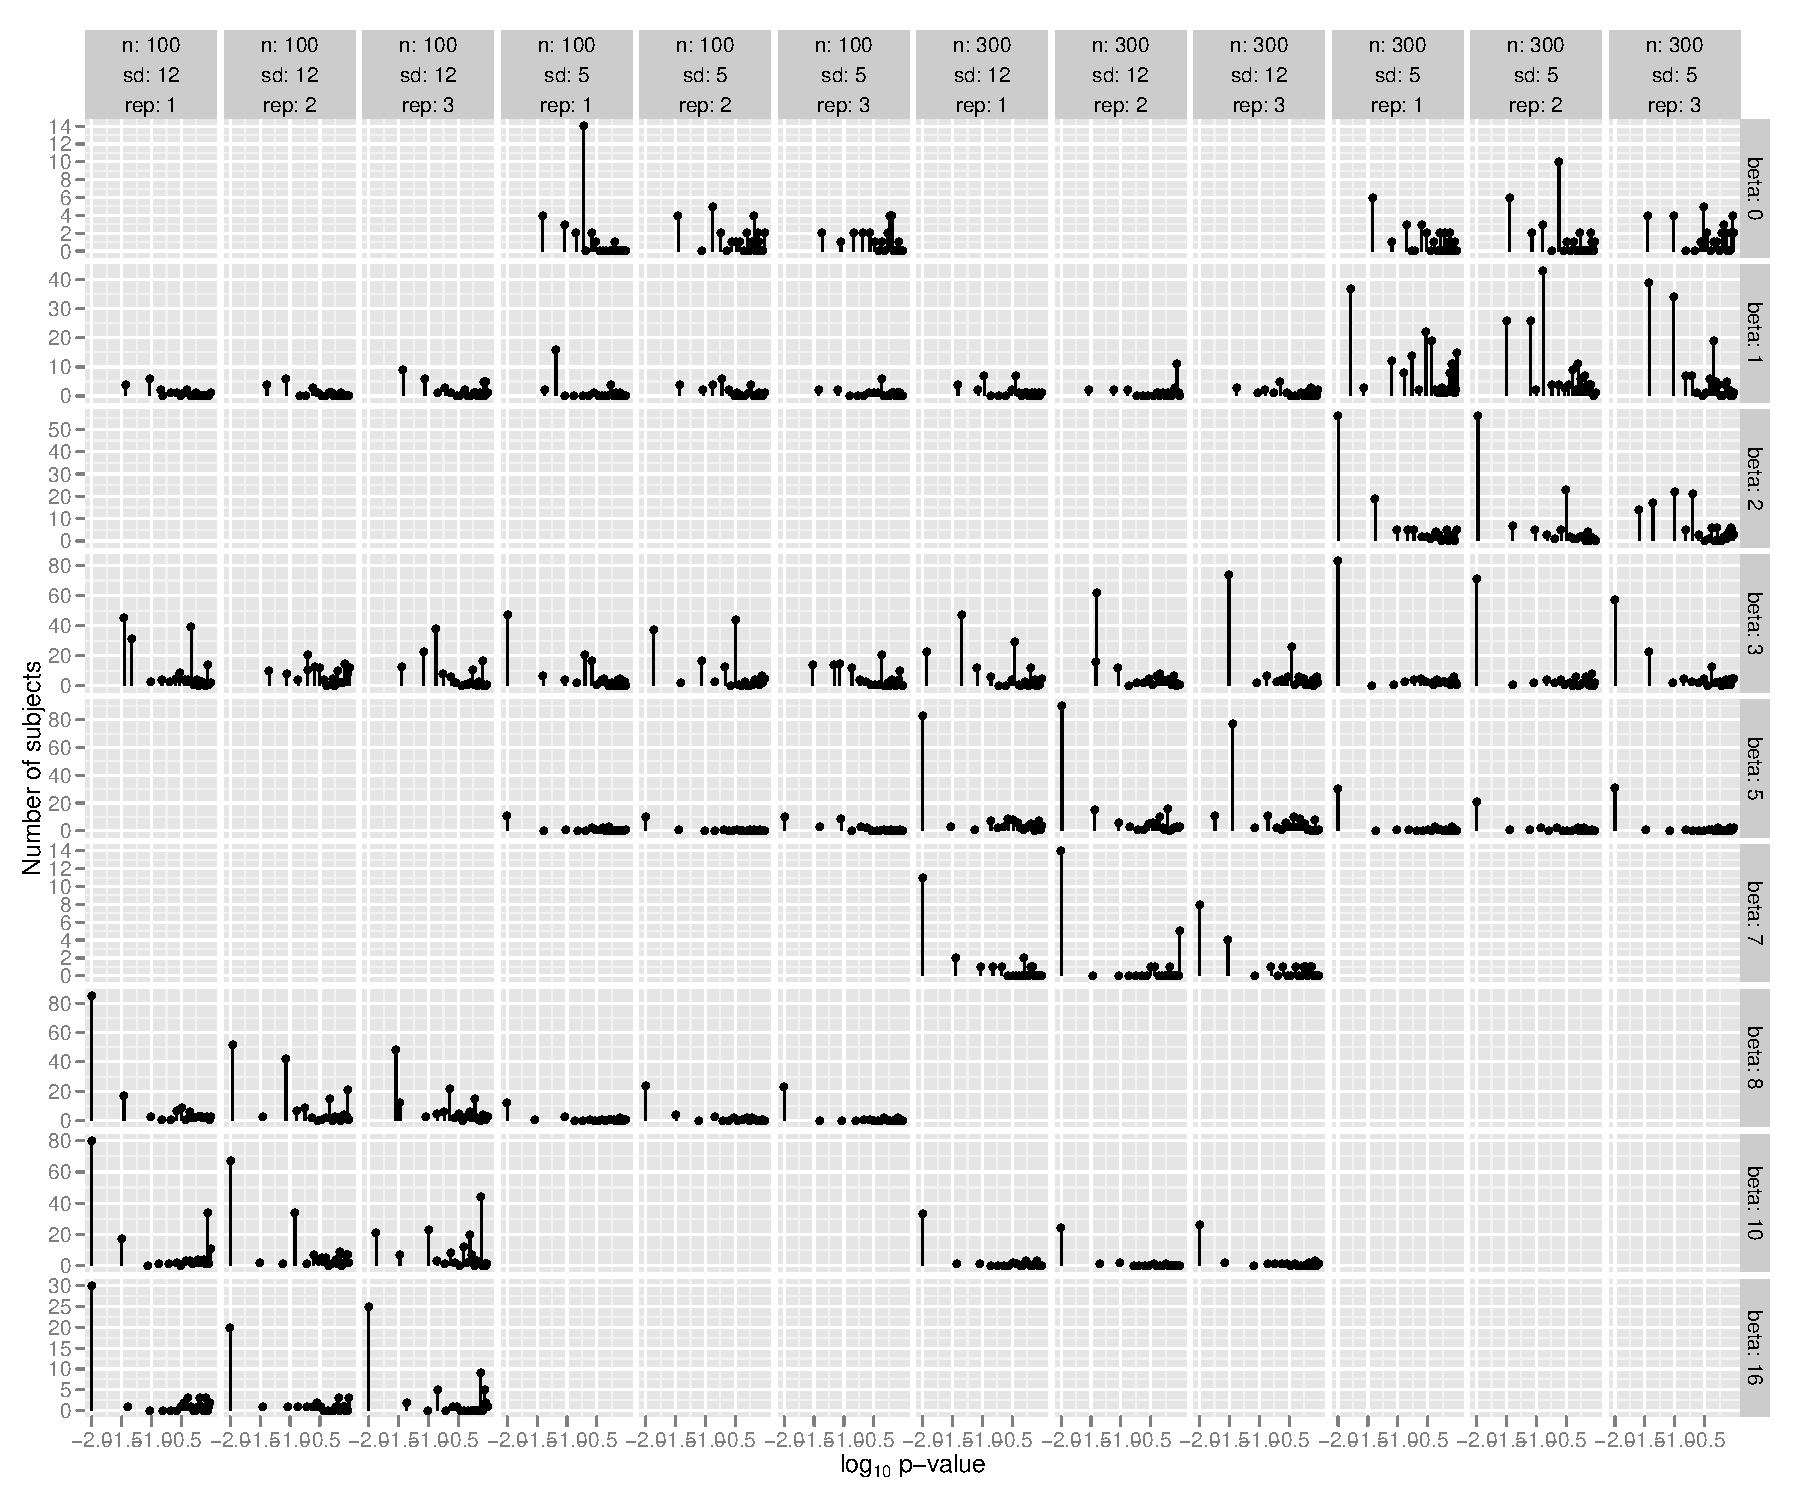
\includegraphics[width=0.95\textwidth]{p_val_log_counts.pdf}
       \caption{Relative frequency of plot picks compared to other plots in the lineup plotted against the $p$-value (on log$_{10}$ scale) of each plot for all of the sixty (60) individual lineups for experiment 1. \blue{Red indicates the} plot with the lowest $p$-value, and \blue{blue indicates the} actual data plot, when it is different from that with the lowest $p$-value. Rows correspond to $\beta$, smallest to largest values from top to bottom. Columns correspond to other experimental treatments, sample size $(n)$, error standard deviation $(\sigma)$, and replicate. Empty cells indicate no lineup for that combination of parameters. Highest counts tend to be the plot in the lineup having the lowest $p$-value.}
       \label{fig:P-val_log}
\end{figure*}

\begin{figure*}[hbtp]
   \centering
       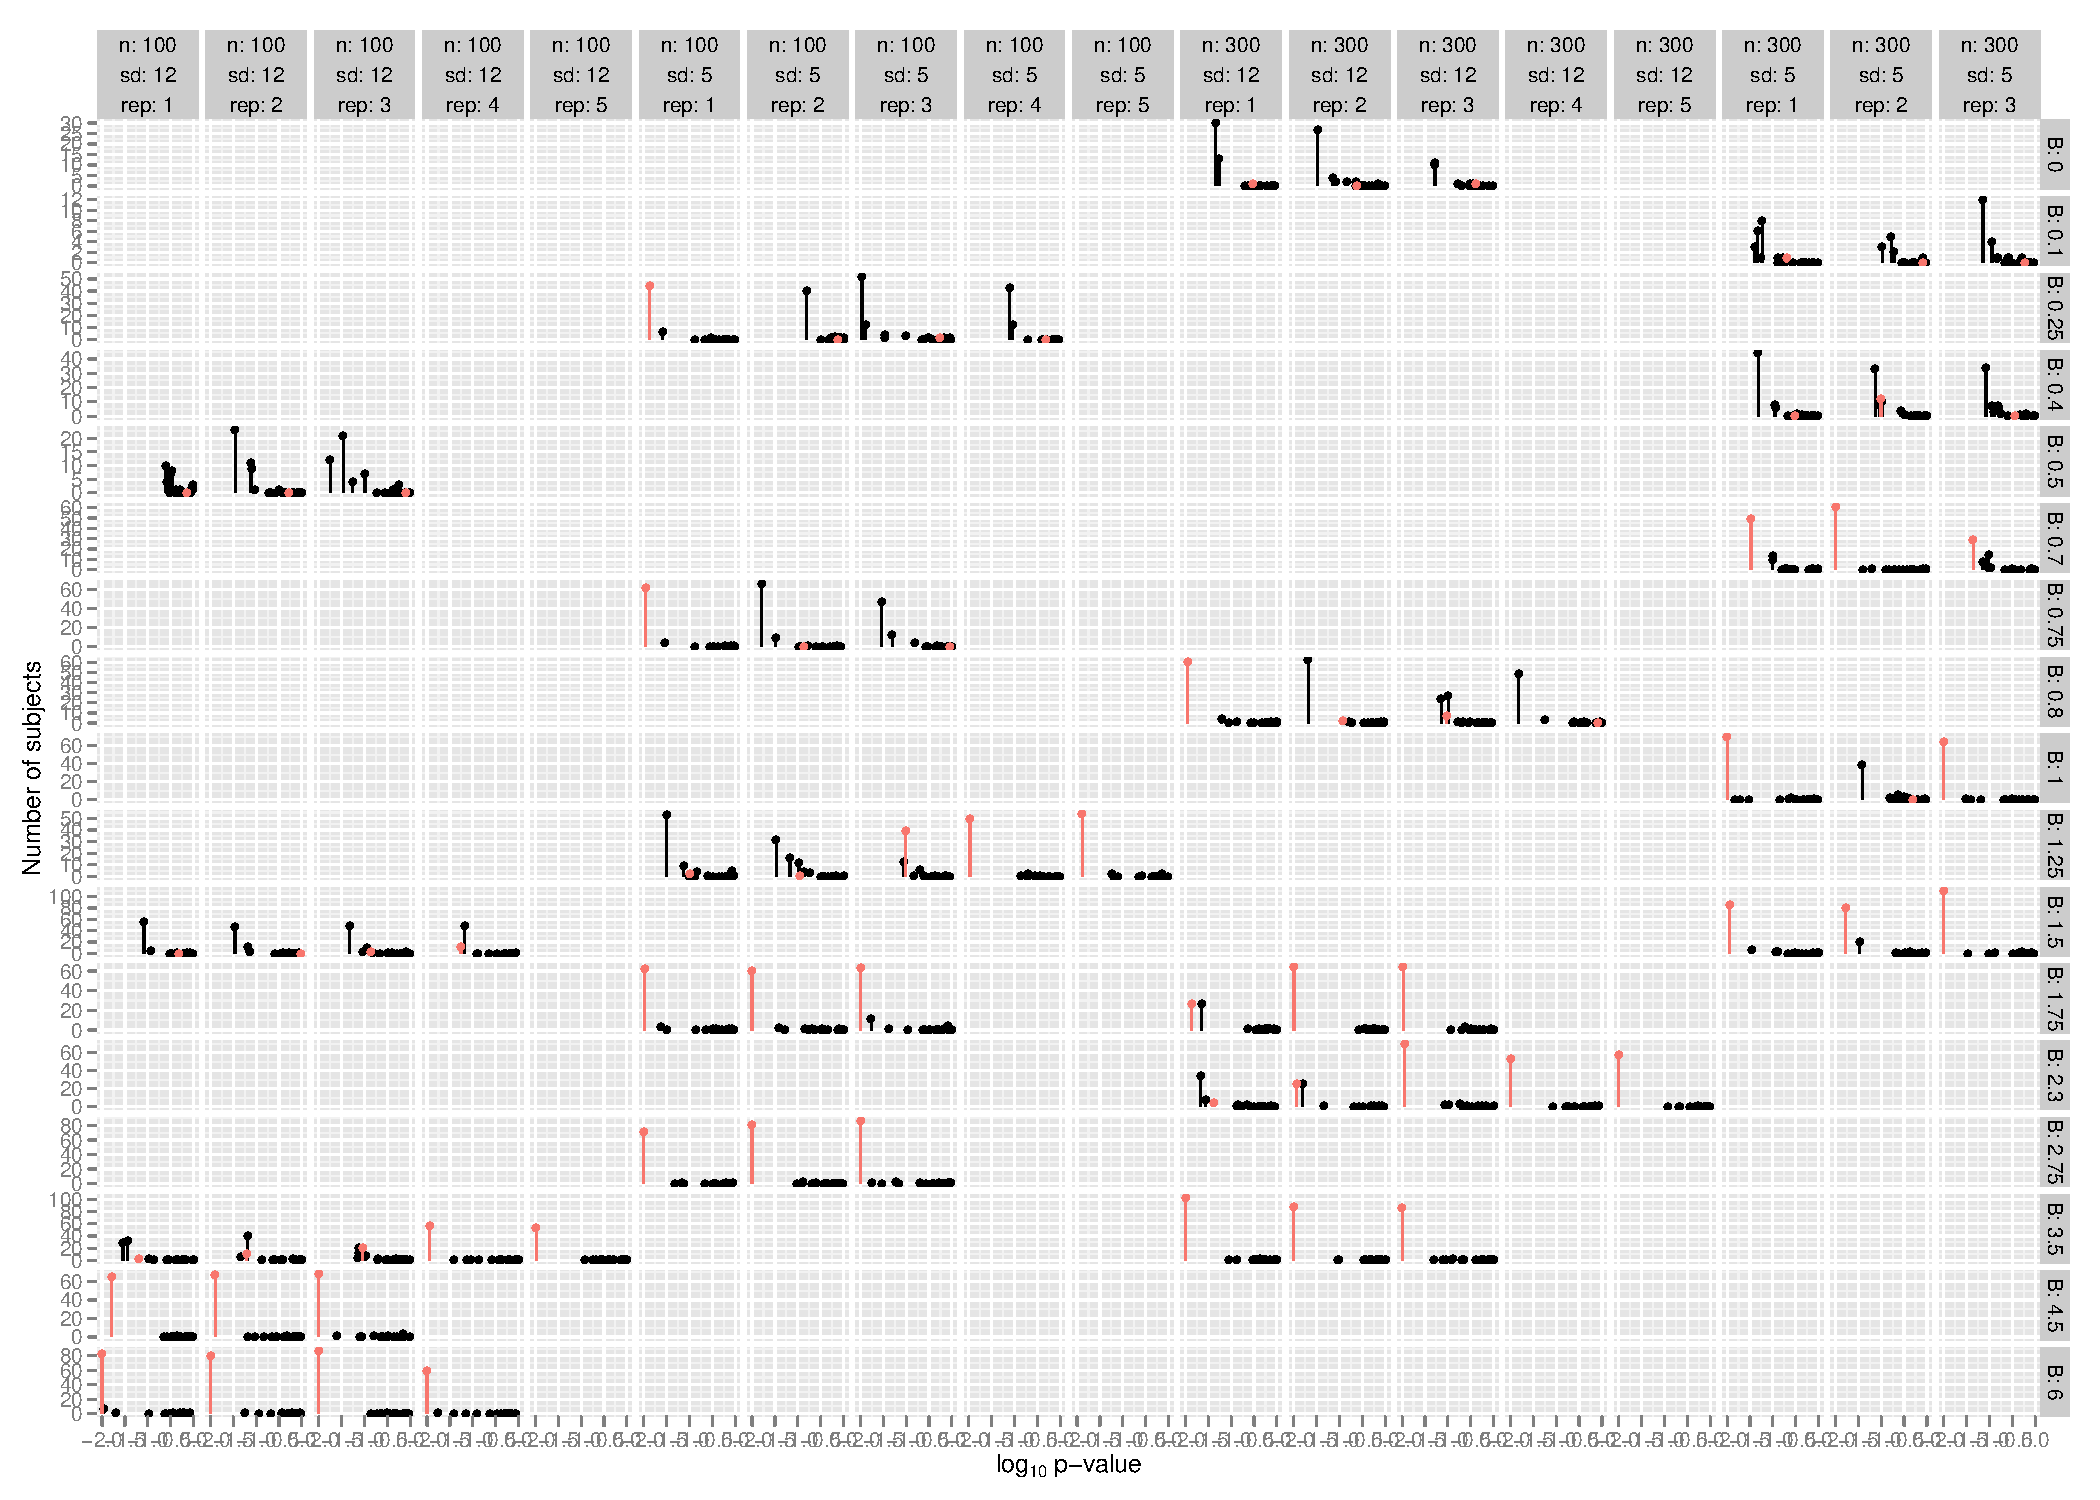
\includegraphics[width=0.95\textwidth]{p_val_log_counts2.pdf}
       \caption{Relative frequency of plot picks compared to other plots in the lineup plotted against the $p$-value (on log$_{10}$ scale) of each plot for all of the seventy (70) individual lineups for experiment 2. \blue{Red indicates the} plot with the lowest $p$-value, and \blue{blue indicates} the actual data plot, when it is different from that with the lowest $p$-value. Rows correspond to $\beta$, smallest to largest values from top to bottom. Columns correspond to other experimental treatments, sample size $(n)$, error standard deviation $(\sigma)$, and replicate. Empty cells indicate no lineup for that combination of parameters. Highest counts tend to be the plot in the lineup having the lowest $p$-value, even more so than for experiment 1.}
       \label{fig:P-val_log2}
\end{figure*}


There are some noticeable exceptions to this rule. In experiment 1, when $\beta=5, n=300, \sigma=12, rep=3$, people tended to pick the plot with the second smallest $p$-value.  Same experiment, when $\beta=0, n=100, \sigma=5, rep=1$ people overwhelming chose a plot with much larger $p$-value. For several of these exceptions, along with several easy lineups, we followed up with a new experiment using an eye-tracker to examine what the observers were looking at in making their choices \citep{zhao:2012}.
(Lineups chosen for the eye-tracker experiment were in experiment 1, (1) $n=100, \beta=3, \sigma=5, rep=1$ (2) $n=100, \beta=5, \sigma=5, rep=1$ (3) $n=100, \beta=10, \sigma=12, rep=1$ and (4) $n=300, \beta=5, \sigma=5, rep=1$, and in experiment 2, (5) $n=100, \beta=3.5, \sigma=12, rep=1$ (6) $n=100, \beta=4.5, \sigma=12, rep=2$ (7) $n=300, \beta=1, \sigma=5, rep=1$ and (8) $n=300, \beta=1, \sigma=5, rep=2$.)


Experiment 3 does not have $p$-values associated with each plot, so the assumption can only be tested with the first two experiments. Practically, this is not an assumption that is explicitly made, because there will not be a $p$-value available. Rather it is assumed that the subject has the ability to select the plot with the most extreme structure. A few of the lineups indicated that occasionally people cue on different patterns, for example, in experiment 1 the lineup $\beta=0, n=100, \sigma=5, rep=1$ (first row, fourth column) many subjects chose the same plot, that had a higher $p$-value. Some of these anomalous lineups were selected for follow-up studies using an eye-tracker to investigate what people were looking at.

%Number of lineups for which most of the subjects picked the data plot based on the minimum $p$-values are shown in Table \ref{tbl:pval_assumption} for both experiment 1 and 2. The $p$-values of lineups which were not chosen based on minimum $p$-value are also very small (close to minimum) as we see in both Figures \ref{fig:P-val_log} and \ref{fig:P-val_log2}. We see the same pattern in Figure \ref{fig:P-val_rank} where the median number of people who pick the data plot with minimum $p$-value (rank 1) are much higher than other ranks.

%\begin{table}[hbtp]
%\caption{Number of lineups for which most people pick the plot with minimum $p$-value. The data used is from screening criteria 1. } 
%\begin{center}
%\begin{tabular}{cccc}
%  \hline
%screening & Experiment & Total &  minimum $p$-value\\ 
%criteria & & lineups & picked by the most \\
%  \hline
%   & 1 &  60 &  37 \\ [-1ex]
%    \raisebox{1.5ex}{1} & 2 &  70 &  60 \\ 
%\hline
%     & 1 &  60 &  38 \\  [-1ex]
%    \raisebox{1.5ex}{2} & 2 &  70 &  61 \\ 
%\hline
%     & 1 &  60 &  38 \\  [-1ex]
%   \raisebox{1.5ex} {3} & 2 &  70 &  60 \\ 
%\hline
%     & 1 &  60 &  41 \\  [-1ex]
%    \raisebox{1.5ex}{4} & 2 &  70 &  60 \\ 
%\hline
%     & 1 &  60 &  39 \\  [-1ex]
%    \raisebox{1.5ex}{5} & 2 &  70 &  60 \\ 
%\hline
%     & 1 &  60 &  40 \\  [-1ex]
%    \raisebox{1.5ex}{6} & 2 &  70 &  60 \\ 
%   \hline
%\end{tabular}
%\end{center}
%\end{table}

%\begin{table}[hbtp]
%\caption{Number of lineups for which most people pick the plot with minimum $p$-value.  } 
%\begin{center}
%\begin{tabular}{ccc} \hline
%screening & \multicolumn{2}{c} {lineups picked by minimum $p$-value} \\
% \cline{2-3}
%criteria & Experiment 1 & Experiment 2 \\ 
%  \hline
%1 & 37 & 60 \\ 
%2 & 38 & 61 \\  
%3 & 38 & 60 \\ 
%4 & 41 & 60 \\ 
%5 & 39 & 60 \\
%6 & 40 & 60 \\ 
%\hline
%Total lineups & 60 & 70 \\  
%\hline
%\end{tabular}
%\end{center}
%\label{tbl:pval_assumption} 
%\end{table}

%\begin{figure*}[hbtp]
%   \centering
%       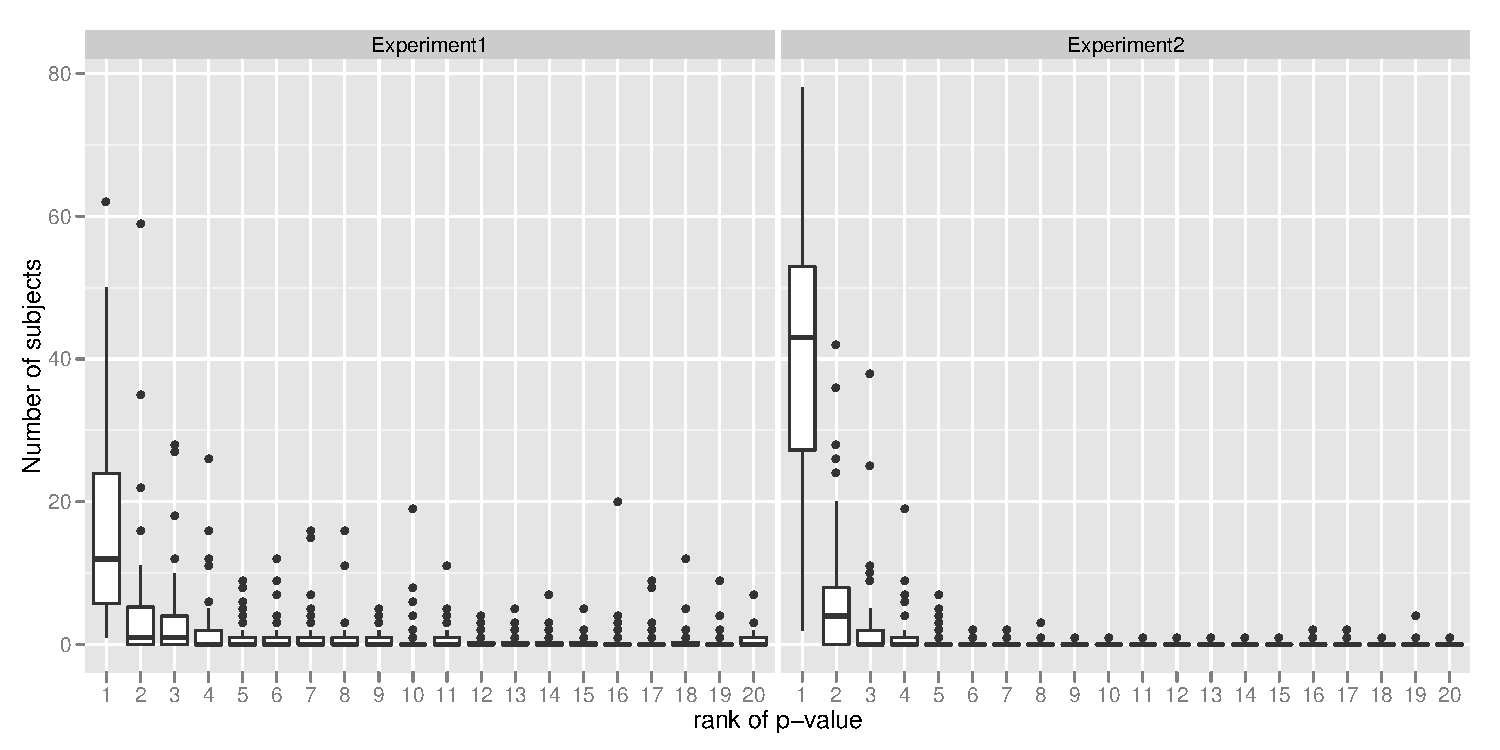
\includegraphics[width=0.95\textwidth]{p_val_rank_counts12.pdf}
%       \caption{Rank of p-values in a lineup of size 20 and the number of subjects choosing that plot in the lineup of experiment 1 and 2 with raw data (screening criteria 1). This indicates that most of the subjects pick the plot with minimum p-value (rank 1). There are subjects choosing the lineups with highest p-value(rank 20) but we can attribute this behavior to the type-I error. Can we?  \green{Maybe don't need this plot}}
%       \label{fig:P-val_rank}
%\end{figure*}



\subsection{How much do null plots affect the choice?}

Visual inference is like other types of computationally intensive test procedures, such as permutation tests, where the statistics from the data are compared with those from null data. But unlike these approaches visual inference is constrained to make the comparison with just a few draws $(m-1)$ from the null distribution. How this small set of null plots influences the subjects choice is important for understanding the reliability of visual inference. If the actual data plot is very different from the null plots, then the null plots should not have much influence on the choice. Measuring the difference, generally, between the plots is almost impossible! But in the controlled setting here we can use $p$-value of the test statistic calculated on the data used in each plot as a proxy for similarity of structure between the plots. 

We have seen that the subjects tend to pick the plot in the lineup that has the lowest $p$-value (Figures \ref{fig:P-val_log}, \ref{fig:P-val_log2}). What we are interested in here is how this pick is affected by the distributin=on of $p$-values of other plots in the lineup, particularly the $p$-value of the null plot with the strongest structure. If there is a null plot with a small $p$-value, or one close to that of the actual data plot, we would expect that subjects have a harder time detecting the actual data plot. Figure \ref{fig:pval_difference} investigates this. The difference between the $p$-value of the actual data is compared with the lowest from the null plots. This is plotted horizontally, and the proportion correct is plotted vertically. Negative values indicate lineups where the actual data plot had a smaller $p$-value than the minimum of the null plots. In experiment 1 (boxplots) there were a lot more lineups where the actual data plot had the smaller $p$-value, but only barely. This caused quite some confusion for subjects, as seen because the variability in the proportion correct is huge for these lineups. Similarly large variability in correctness can be seen in the results of experiment 2 (scatterplots) except that the greater range of of differences in $p$-values shows the strength of subject's ability to pick the plot with most structure. Figures \ref{fig:P-val_log}, \ref{fig:P-val_log2} show a little more complicated story. When there is a big difference between the $p$-values (eg experiment 1, $\beta>7$) the subjects' as a force choose the same plot. when there is less difference the distribution of counts is much more evenly spread between plots (eg experiment 1, $\beta=1$). 

%\blue{In the previous section we noticed that subjects tend to pick the plot with the lowest $p$-value. If a null plot has data that, by chance because the sample is a random draw from the null, has a smaller $p$-value than the actual data, we would expect that there is a strong possibility that an subject will pick this null plot instead of the actual data plot. Figure \ref{fig:pval_difference} investigates this for the data collected in experiments 1 and 2. The plots display the proportion of subjects who choose the actual data plot against the $p$-value of the actual data minus the lowest seen in the null data. A small negative value of the difference means that the $p$-value of the actual data is smaller than that of the null data. If there is a big negative difference we'd expect to see that the subjects would more often make the correct choice of plot. When there is a large positive difference, subjects fail to pick the correct plot. If however, there is little difference between the $p$-values then we'd expect to see more confusion in the choices. That is why we see a big range of proportion correct where difference is close to zero in Figure \ref{fig:pval_difference}.}

%\green{Something is definitely not right! The code looks like it does actual data p-value - min(null $p$-value). But how can you get a difference of 0.8 from this??} \blue{It is possible theoretically! Suppose data plot $p$-value is larger than 0.8. Under null hypothesis, $p$-value $\sim U(0,1)$. Thus min(null $p$-value) could be close to zero by chance producing this large difference. And this has happened in both experiment 1 and 2.}

 %\green{Is this really pct correct, or 1-pct correct? \blue{This is proportion correct}. When there is a big diff in p-value almost no-one gets it right! Maybe it is just a scale issue?} \blue{In fact this is what we expect. If there is large difference that means data plot $p$-value is large while minimum $p$-value is very small. This should lead people to pick the wrong plot. Our minimum $p$-value assumption basically says this fact, right?}. We see that when there is a big difference between the $p$-values subjects choose the actual data plot more often.

%Mahbub, could you have a look at the lineups, and compute the difference between the data plot's $p$-value and the  smallest $p$ value of a null plot, and plot that in a scatterplot against proportion correct? Thanks! 

In practice, $p$-value is not going to be a valid way to compare plots. Rather metrics that can measure how graphical elements from one plot to another are perceived similarly are needed. This is investigated in \citet{niladri:2012}. Here numerical measures of the similarity between plots are proposed to provide quality metrics for lineups.


\begin{figure}[hbtp]
   \centering
       \scalebox{0.70}{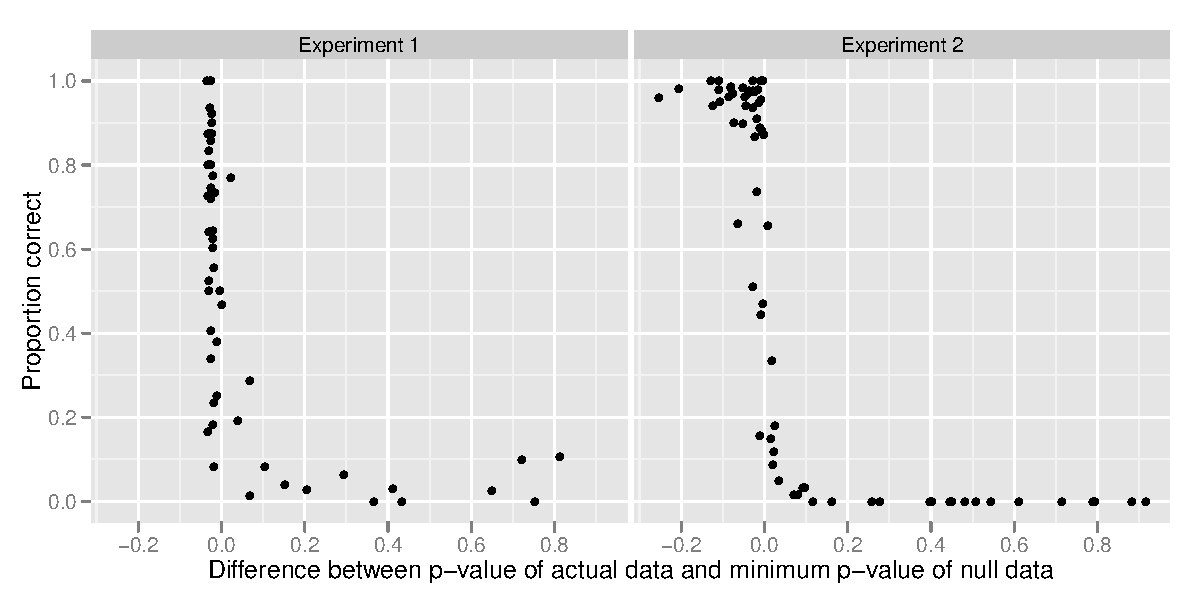
\includegraphics{pval_difference.pdf}}
       \caption{Investigating how the strength of structure in the null plots affects the choice of the actual data plot. Difference between the data plot's $p$-value and the  smallest $p$ value of a null plot vs proportion correct. Negative values indicate the $p$-value of the actual data plot are smaller than those of all of the null plots. Close to zero shows a wide range in the proportion correct, suggesting that when at least one null plot has structure almost as strong as the actual data plot, subjects had a difficult time in making their choice.}
       \label{fig:pval_difference}
\end{figure}

\subsection{Type III error}~\label{sec:TypeIII}


A little known error amongst statisticians is what was coined as Type III error in \citet{mosteller:48}. This occurs when the null hypothesis is rejected for thw rong reason. Experiment 3 is prone to this type of error. Observers were asked to identify the plot that had the largest slope, either positive or negative. But the actual data plot had a cluster of points, the contamination that forced the conventional test to fail to see any trend. For the human eye this cluster of points is probably as visible as the association between the remaining points, leading the observer to detect the actual data plot by looking for the cluster instead of the slope. This would be considered to be a Type III error because it is not what was requested, but it still gives the correct answer. This is not a problem with the lineup protocol, because we want observers to react to anything that sets the the actual data plot apart. Here, in the controlled but simple setting, it is of interest to see what observers cued to in the actual data plot. 

Figure \ref{fig:power_loess_effect} indicates that Type III error might be occurring in experiment 3: correct identification of the actual data plot is not positively associated with effect size. Teasing this out of the results is possible by looking at the reasons observers gave for their choices. Observers were provided with four possible reasons to use for their choice:


\begin{enumerate} \itemsep 0in
\item Most different plot
\item Visible trend
\item Clustering visible
\item Other
\end{enumerate}


\noindent with the possibility to use more than one. The task requested subjects to identify the plot that had the largest slope, which would correspond to choosing ``visible trend'' (2) as the reason for their choice. Reasons 1 or 3 would be indicative of Type III error. Figure \ref{fig:choice_reason} explores the reasons subjects gave for their choices. If there were no Type III errors committed, we would expect that people overwhelmingly using ``visible trend'' as their reason, or at least, when they use this reason they overwhelmingly correctly choose the actual data plot. This is not what we see. At left, are the reasons subjects gave for their choices --- 123 means that they gave all three reasons. The horizontal axis shows proportion of times that subjects correctly chose the actual data plot, and the reasons are sorted from most accurate to least accurate. The size of the point corresponds to the number of subjects putting this as the reason. Subjects that chose all three reasons almost always chose the actual data plot. This was followed by using 1 and 3, and then 1 and 4. The most common reasons given were reasons 1-3 individually, and the accuracy for these reasons ranged from 75\% for reason ``most different plot'' to 60\% for ``visible trend''.
At right is a simplified view, containing just the four possible reasons -- if the subject chose one of these, regardless if they also chose another reason it is counted. ``Visible trend'' comes in third. This is strong evidence that for many subjects even though they are correctly choosing the data plot, often they are cueing to other structure in the plot than the trend, making a Type III error. 


%It is interesting to calculate the proportion of observers who choose the correct plot, but use reasons 1 or 3, relative to reason 2. Figure \ref{fig:choice_reason} examines this. For observers who chose the actual data plot, the proportions for the three reasons are shown. It can be seen that the most common reason was ``most different plot'' (1), followed by clustering visible (3), with ``visible trend'' coming in third. \green{What about other??} \blue{Not many people chose other as we see in Figure \ref{fig:choice_reason}.}


%This might be an indication that participants were not considering slope as distinguishing feature for the data, but the apparent clustering, i.e. the null hypothesis is being rejected, but not for the reason of the slope -- which the experimental setup was asking for --  leading to a type III error of correctly rejecting the null hypothesis for the wrong reason', as defined by \citet{mosteller:48}

%\green{Not sure that this goes here, but something needs to be said about Type III.} 

%\blue{We also see this feature in figure \ref{fig:choice_reason}}.
%\hh{Mahbub, it's not directly fig \ref{fig:choice_reason} - it's actually the lineup corresponding to the large outlier at (0.2,  0.6) in the left panel of fig \ref{fig:choice_reason}.}

\begin{figure}[hbtp]
   \centering
%       \scalebox{0.60}{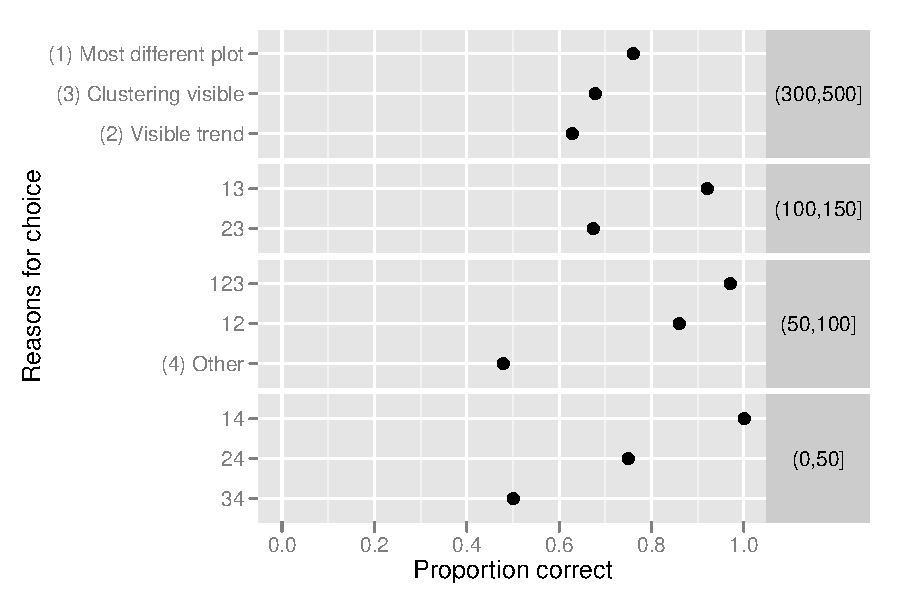
\includegraphics{choice_reason.pdf}}
%       \scalebox{0.60}{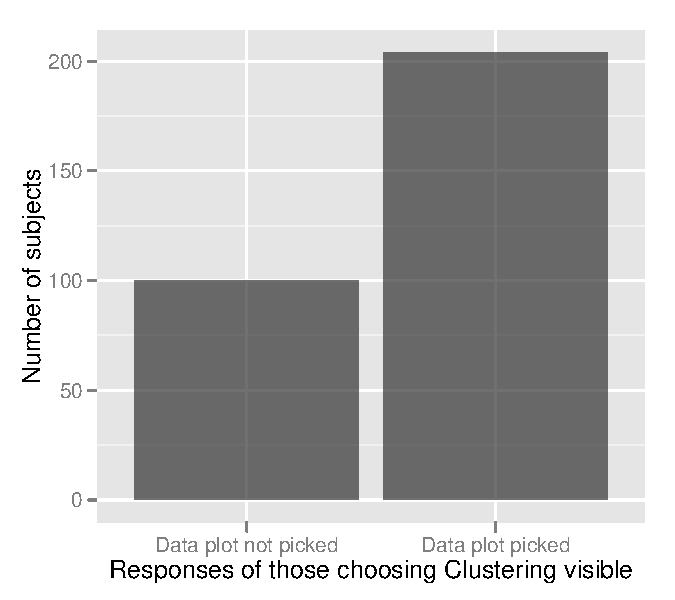
\includegraphics{choice_reason_count.pdf}}
       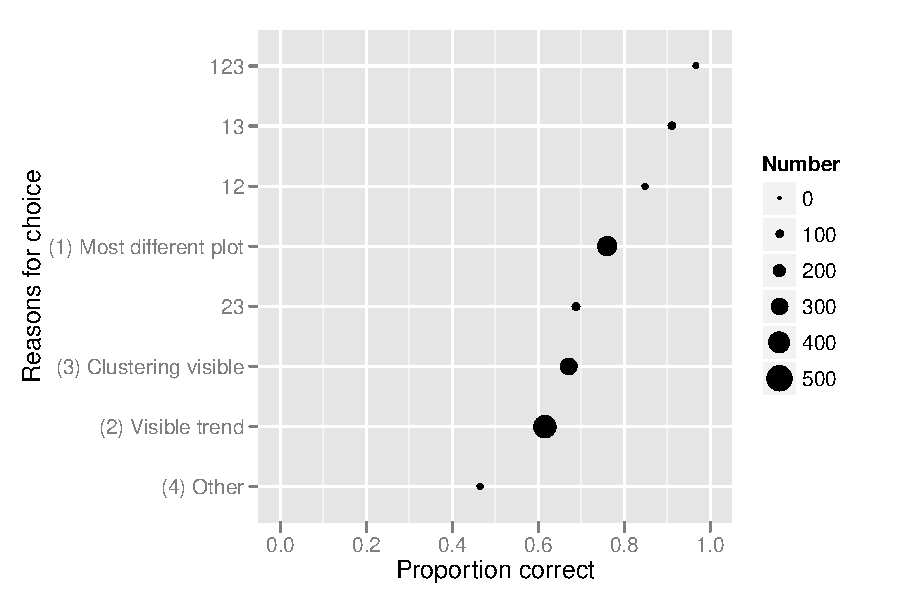
\includegraphics[width=0.45\textwidth]{choice_reason2.pdf}
       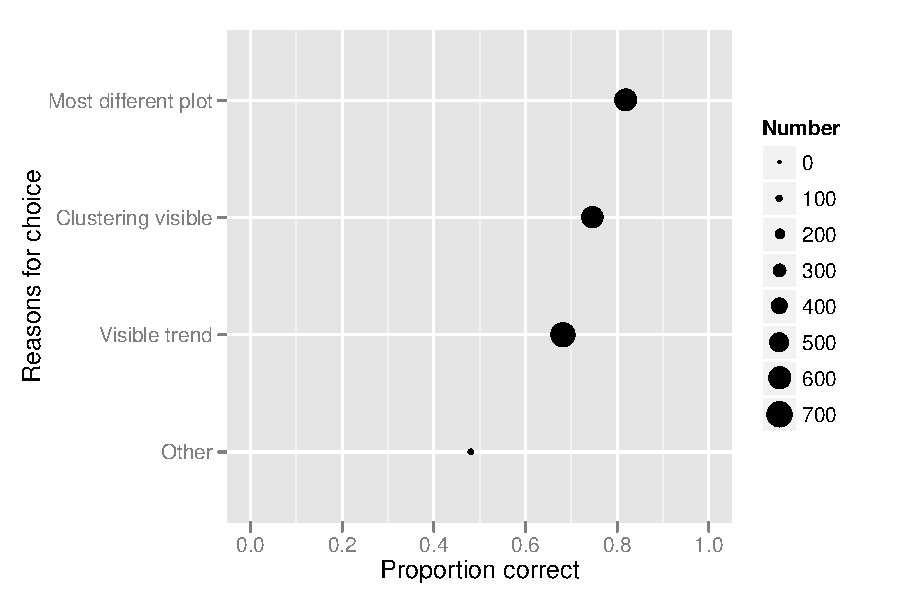
\includegraphics[width=0.45\textwidth]{choice_reason3.pdf}
       \caption{Exploring the reasons for plot choices for experiment 3, to examine the occurrence of Type III error. The vertical axis shows the reasons. At left, all subjects choices are shown, and reason 123 means all three reasons are used. At right, if the subject used a reason, regardless if they also used more than this reason, they are counted. The horizontal axis shows the proportion of times the subjects correctly chose the actual data plot. Size of the point corresponds to the number of subjects using that reason.}
       \label{fig:choice_reason}
\end{figure}

For visual inference, making a Type III, is not actually a problem. It is only a possibility in this experiment because we are working with known structure. In the real setting, we are excited to see observers detecting the actual data plot, and curious about how they detect it, with all possible reasons encapsulated in the alternative hypothesis. This does show the importance of the qualitative answers that observers give for their choices.

\section{Conclusions}


%\begin{itemize} \itemsep 0in
%\item Summarize the key pieces of the paper again, especially the major findings

It is widely accepted that statistical graphics has important use in exploratory data analysis and model diagnostics. This paper has demonstrated that statistical graphics can be used in statistical inference and validates the lineup protocol proposed by \citet{buja:2009} as a formal framework to accomplish that. The simulation study showed that even in the situation where the conventional test has its assumptions met, visual inference is comparable. The results also suggest that when the underlying assumptions of a conventional test do not hold, visual inference will perform well. 

Power of visual tests can be estimated in different ways, which was explained in this paper. If it is assumed that observers tend to pick the plot with the strongest signal, which was consistent with the experimental data, the power of visual test can be obtained theoretically.  Interestingly, the theoretical power of visual test is close to that of conventional test in the conditions tested in this paper.

%\item Explain caveats, nuances, advantages with the work

One of the critical parts in visual testing is appropriate selection of a statistic for the hypothesis of interest -- that means an appropriate choice of plot for the analytical purpose.  A good test statistic is expected to reveal structure if the null hypothesis is not true. Small differences in plot choices such as color, orientation, and mapping of data values to graphical elements of the plot can make a difference. This is related to research in a grammar of graphics \citep{wilkinson:1999,hadley:2009}, which helps to ensure good practices. %This is the part of our ongoing and future research.

The question that is posed to observers can affect the abililty to evaluate lineups. In these experiments subjects were asked very specific questions, because the purpose was to compare with very specific conventional testing. In practice, the question posed will be very general to allow observers to choose plots with any remarkable features, which enables the data mining discovery process.

% when evaluating the lineup: this question can be lined up with the alternative hypothesis of a classical testing scenario. If we are interested in the reason why participants picked a plot as the most different, we need to collect and evaluate this information in the study. This has to be done very carefully, as any suggestions for reasons also lead the observer  what patterns to look out for.}
% By delivering an appropriate question may reduce the type III error in an appropriate scenario.}

Even though a single observer can evaluate a lineup, as suggested in the initial lineup protocol, this work recommends having multiple observers. This ensures the ability to obtain a good estimate of the $p$-value for the test, and more confidence in the decision.

Experimental subjects in the simulation study came from various level of education, both genders and many different ages. Many subjects had little background in statistics, and were not necessarily aware of statistical plots. Yet the results were good. We expect that visual inference could be a useful tool for high school students to learn about randomness as a primer to statistical thinking. A major advantage of visual statistical inference is that it is intuitive, as illustrated by the performance of subjects with limited education, and it is may make statistics fun to learn. 

The performance of subjects was quite varied, but consistent. No restrictions were placed on Turk workers, in terms of abilities. There were clearly some subjects who performed very badly, but it was very interesting to see that there were some super-observers, people who detected the actual data plot at a rate better than that of the power of the best conventional test. 
 It would be interesting to see how well trained subjects might perform. Prior to the Turk experiments, we conducted pilot studies using local graphics experts and obtained good results, indicating that training in data visualization might be helpful for visual inference. Future work might explore this.

%\item Describe the next steps of the work, and possible ideas for future extensions

When there is no conventional test available, visual testing procedures can be used due to its few assumptions and non-parametric nature. We have successfully used the procedures informally for local projects. It is hoped that this proves to be extremely valuable in data mining applications, and exploratory analyses, where there are no exising gauges of statistical significance. The lineup protocol operates similarly to general tests, such as two-sided, analysis of variance $F$-tests, and Wilks $\Lambda$ for multivariate analysis of variance. If the null hypothesis is rejected, it is generally that we can say that ``there is something there'' but not specifically what it is in the data that triggers the rejection. Follow-up questions on the reasons provide qualitative insight. Multiple comparisons are often done to refine and understand the results of the general conventional testing, and perhaps some similar approaches might be developed for visual inference. 

%Such a scenario could be the inference with small sample size with large number of covariates, data mining findings or even in genetic research where many covariates restrict the available inference very conservative for simultaneous testing (required $p$-value is very small to be able to reject $H_0$). The direction of future research would be to study that and apply the methods in those areas.


%The purpose of this paper has been to examine the effectiveness of visual inference methods in direct comparison to existing inference methods. We need to be clear that this is not the purpose of visual inference generally: visual methods should not be seen as competitors to conventional inference.  The purpose here, is to  establish properties and  efficacy of visual testing procedures in order to use them in situations where conventional tests cannot be used. For this experiment the effect of $\beta_2$ was examined using side-by-side boxplots. Future experiments will be conducted to compare other regression parameters as described in Table \ref{tbl:stat_multiple} and assess sensitivity of power to modeling conditions.

%\green{Mention the possibility of a visual skills test, to select the workers that are better qualified, to implement the lineup protocol in practice. Along the lines of the Army tests that Susan brought to the working group. \blue{While recruiting subjects from the Amazon Mechanical Turk web site we did not put any restriction on the skill levels of the subjects. Thus anyone from any background could participate the experiment. It would be interesting to see how well the trained subjects performs. Many pilot studies with advanced knowledge of statistical graphics as well as statistics indicates that the performance is very good for trained subjects. One of our future work would be to examine this in details. For this we are planning to trained Turk subjects with specific graphics and educate them what pattern a specific graphics may show. After being trained they may have to pass the qualification test before participating the experiment. Even though we did not do this, it is very common to Turk subjects to go through this process for various other tasks they do in the Turk web site.}.

%Discuss the purpose of randomly generating data null plots, rather than selectively sampling from the null distribution.}

%In practice there is no correct answer. In these experiments we controlled the effects that observers saw, so there was a correct choice in each case. In the real setting, there is not correct choice, just whether the actual data plot stands apart from the rest, so that the observer can find it. And subjects would provide open-ended answers for their choice of plot. 

%What are your suggestions for future experiments, and next steps of the research?

%\paragraph{Acknowledgement:}
%This work was funded in part by National Science Foundation grant DMS 1007697.

%\bibliographystyle{plain}
%\bibliographystyle{plainnat}
\bibliographystyle{asa}
%\bibliographystyle{ieeetr}
\bibliography{references}

%\end{multicols}

\end{document}  %End of document.



\section*{Appendix}

\begin{table}[hbtp]
\caption{Selection of 10 lineups for a person to evaluate in the simulation experiment with discrete covariate described in section \ref{sec:category}.} 
\centering
\begin{tabular}{c c c c  c c c}
\hline\hline
Difficulty& \multicolumn{3}{c}{parameter combination}& Number of evaluations &Total number  & number of lineups\\
level & $n$ & $\sigma$ & $\beta$ &required($n_{\gamma}$) & of lineups & randomly shown \\
\hline
easy&100& 5&8 & 1& 12 & 1\\
&100&12&16 &1&&\\
&300& 5&5 &1&&\\
&300&12&10 &1 &&\\
\hline
medium&100& 5&3 &203 & 9 &2\\
&300& 5&2,3 & 97, 1&&\\
\hline
hard&100&12&3,8,10 & 277, 126, 23& 18 &6\\
&300& 5&1 & 371 &&\\
&300&12&3,5& 375,74 &&\\
\hline
mixed&100& 5&1,5,0& 214, 2,73 & 21 &1\\
&100&12&1& 100& &\\
&300& 5&0 & 73&&\\
&300&12&7,1& 2, 152&&\\
\hline
Total &&&&&60&10\\
\hline
\end{tabular}
\label{tbl:dist_lineup1}
\end{table} 



%\begin {abstract} 
%Statistical graphics play a crucial role in exploratory data analysis, model checking and diagnosis. Until recently, there were no formal visual methods in place for determining statistical significance of findings. This changed when Buja et al. (2009) conceptually introduced the lineup protocol for formal tests of visual findings. In this paper this is taken a step further by refining the terminology of visual inference, framing the protocol in a context that allows direct comparison with conventional tests, in scenarios when a conventional test exists, and it is used to compare the performance of the lineup protocol against conventional statistical testing in the scenario of fitting linear models. A human subjects experiment is conducted using simulated data to provide controlled conditions. Results suggest that the lineup protocol provides results comparable to the conventional tests, out-performs them when data is contaminated, and, there may be some super-individuals who yield better power than the conventional test even in the most difficult trials.
%\end {abstract}

\end{document}
